%=====================================================
% PREÂMBULO - CONFIGURAÇÕES GERAIS DO DOCUMENTO
%======================================================
\documentclass[12pt, a4paper, openright, oneside, brazilian]{abntex2}

% --- PACOTES DE CODIFICAÇÃO ---
\usepackage{fontenc}
\usepackage[utf8]{inputenc}

% --- PACOTES DE LAYOUT E FORMATAÇÃO (ABNT/UNESP) ---
\usepackage[left=3cm, top=3cm, right=2cm, bottom=2cm, headsep=1.5cm]{geometry}
\usepackage{indentfirst} % Indenta o primeiro parágrafo de cada seção
% Usando o comando nativo da classe memoir (base do abntex2) para espaçamento 1,5 [1]
\OnehalfSpacing
% --- PACOTES DE BIBLIOGRAFIA (ABNT) ---
\usepackage{csquotes}
% Opções simplificadas para máxima compatibilidade.
\usepackage[backend=biber, style=abnt]{biblatex}
\addbibresource{bibliografia.bib} % Seu arquivo.bib

% --- PACOTES MATEMÁTICOS ---
\usepackage{amsmath}
\usepackage{amssymb}
\usepackage{mathtools}

% --- PACOTES PARA TABELAS E FIGURAS ---
\usepackage{graphicx}
\graphicspath{{../../}{imagens/}}

\usepackage{booktabs}
\usepackage{multirow}
\usepackage{array}
\usepackage[table]{xcolor}
\usepackage{caption}
\usepackage{subcaption}
\usepackage{float}
% --- Configurações automáticas de posicionamento ---
\renewcommand{\topfraction}{0.9}    % Permite que figuras ocupem até 90% do topo da página
\renewcommand{\bottomfraction}{0.8} % Permite que ocupem 80% da base
\renewcommand{\textfraction}{0.05}  % Permite que o texto ocupe apenas 5% da página se necessário
\renewcommand{\floatpagefraction}{0.85} % Só cria uma página só de figuras se elas ocuparem 85% dela
\usepackage[section]{placeins} % Muro invisível automático no final de cada seção
\usepackage{tikz}
\usetikzlibrary{shapes.geometric, arrows.meta, positioning, automata, backgrounds, calc}
\usepackage[american, siunitx]{circuitikz}
\captionsetup{
    format=plain,
    justification=justified,
    singlelinecheck=false,
    font=normalsize,
    labelfont=bf,
    labelsep=period
}
\newcommand{\legendafonte}[1]{{\footnotesize\caption*{Fonte: #1}}}

% --- PACOTES ADICIONAIS ---
\usepackage{ragged2e}
\usepackage{soul}

% --- QUEBRA DE LINHA E TIPOGRAFIA ---
\usepackage{microtype}
\usepackage{xurl}
\setlength{\emergencystretch}{3em}
\tolerance=2000
\pretolerance=1000
\makeatletter
\let\breakable@origtexttt\texttt
\DeclareRobustCommand{\breakabletexttt}[1]{%
  \ifmmode
    \breakable@origtexttt{#1}%
  \else
    \begingroup
    \ttfamily
    \let\breakable@us\_
    \def\_{\breakable@us\allowbreak}%
    #1%
    \endgroup
  \fi
}
\let\texttt\breakabletexttt
\newcommand{\code}[1]{{\UrlFont\nolinkurl{#1}}}
\makeatother

% --- CONFIGURAÇÃO DE HIPERLINKS ---
\hypersetup{
    colorlinks=true,
    linkcolor=black,
    citecolor=black,
    urlcolor=black,
    pdftitle={Desenvolvimento e Análise de um Controlador Eletrônico de Velocidade para Motores de Corrente Contínua Sem Escovas},
    pdfauthor={Enzo Luiz Fernandes},
    bookmarksopen=true
}

%=====================================================
% METADADOS DO TRABALHO (PARA CAPA E FOLHA DE ROSTO AUTOMÁTICAS)
%=====================================================

\titulo{Desenvolvimento e Análise de um Controlador Eletrônico de Velocidade para Motores de Corrente Contínua Sem Escovas}
\autor{Enzo Luiz Fernandes}
\instituicao{
  Universidade Estadual Paulista "Júlio de Mesquita Filho"
  \par
  Faculdade de Engenharia de Ilha Solteira
  \par
  Departamento de Engenharia Elétrica
}
\local{Ilha Solteira}
\data{2026}
\orientador{Prof. Dr. Guilherme de Azevedo e Melo}
\tipotrabalho{monografia}
\preambulo{Trabalho de Graduação apresentado ao Departamento de Engenharia Elétrica da Faculdade de Engenharia de Ilha Solteira, da Universidade Estadual Paulista "Júlio de Mesquita Filho", como parte dos requisitos para obtenção do título de Bacharel em Engenharia Elétrica.}

\begin{document}

% --- ELEMENTOS PRÉ-TEXTUAIS --
\begin{capa}
    \centering
    {\ABNTEXchapterfont\large\imprimirinstituicao}
    \vspace{1.5cm}
    
\includegraphics[width=9cm]{imagens/logoUNESP.jpg}
    \vfill
    {\ABNTEXchapterfont\large\imprimirautor}
    \vfill
    \begin{center}
    {\ABNTEXchapterfont\bfseries\LARGE\imprimirtitulo}
    \end{center}
    \vfill
    {\large\imprimirlocal}
    \par
    {\large\imprimirdata}
    \vspace*{1cm}
\end{capa}

\imprimirfolhaderostonostar{\folhaderostoname}
\begin{fichacatalografica}
    % PLACEHOLDER -- substituir pelo texto gerado em
    % https://www.biblioteca.unesp.br/ficha/
    \vfill
    \begin{center}
        \textbf{[Ficha catalogr\'afica -- inserir texto da Biblioteca FEIS/Unesp]}
    \end{center}
    \vfill
\end{fichacatalografica}

% Folha de Aprovação
\begin{folhadeaprovacao} 
\begin{center}
{\ABNTEXchapterfont\large\textsc{\imprimirautor}}
\par\vspace{\onelineskip}
{\ABNTEXchapterfont\Large\bfseries\imprimirtitulo} 
\end{center} 
\vspace{1cm} 
\hspace{.45\textwidth} \begin{minipage}{.5\textwidth} 
\imprimirpreambulo 
\end{minipage} 
\vspace{1cm}
\par\vspace{\onelineskip}
Trabalho aprovado. \imprimirlocal, \imprimirdata: 

%Assinaturas 
\assinatura{\imprimirorientador \\UNESP} 
\assinatura{Assinatura 2\\ UNESP} 
\assinatura{Assinatura 3 \\ UNESP} 

\end{folhadeaprovacao}

% RESUMO E ABSTRACT
\begin{resumo}
    Este trabalho apresenta o desenvolvimento e a análise de um protótipo de controlador eletrônico de velocidade (ESC) para motores de corrente contínua sem escovas (BLDC), utilizando o microcontrolador ESP32. A fundamentação teórica aborda a conversão eletromecânica, as constantes $K_T$, $K_V$ e $K_e$, a comutação trapezoidal de seis passos, a modulação por largura de pulso (PWM), a partida \textit{sensorless}, o controle proporcional-integral (PI) e os principais aspectos de eletrônica de potência e software embarcado aplicáveis ao acionamento. A metodologia seguiu uma abordagem de engenharia de sistemas, envolvendo o dimensionamento de uma ponte inversora trifásica, do barramento DC, dos circuitos de acionamento por \textit{gate driver}, das proteções de sobrecorrente e subtensão, do sensoriamento de corrente, da reconstrução de neutro virtual e do condicionamento da força contraeletromotriz para futura detecção de cruzamento por zero (ZCD). Também foram desenvolvidos a PCB protótipo e um \textit{firmware} modular em PlatformIO/FreeRTOS, com camada de abstração de hardware, máquina de estados, comutação seis passos via MCPWM, PWM a $20\,\text{kHz}$, malha de controle a $1\,\text{kHz}$ e interfaces de comando e telemetria. Os resultados incluem validações em LTSpice, análise dos esquemáticos e da PCB, testes estáticos de bancada e avaliação da arquitetura de \textit{firmware}. As simulações confirmaram os caminhos de corrente, o estado de alta impedância da fase não energizada e a necessidade do banco de capacitores do \textit{DC link}. Os ensaios estáticos validaram a manipulação do MCPWM, o tempo morto implementado por \textit{hardware} e as rotinas de proteção. Entretanto, a validação dinâmica integral com motor em rotação foi interrompida após o ensaio a vazio indicar consumo transiente excessivo e disparo da proteção da fonte, compatíveis com falha estrutural no estágio físico de potência. Assim, o objetivo geral foi parcialmente atingido: a base teórica, eletrônica, computacional e de \textit{firmware} foi consolidada e documentada, enquanto a operação completa do ESC permanece dependente de uma nova iteração do \textit{hardware} de potência.
    \par\vspace{\onelineskip}
    \noindent\textbf{Palavras-chave:} Motor BLDC; Controlador Eletrônico de Velocidade; ESP32; Comutação de Seis Passos; Controle Embarcado.
\end{resumo}

\begin{resumo}[Abstract]
\begin{otherlanguage*}{english}
This work presents the development and analysis of an electronic speed controller (ESC) prototype for brushless direct current (BLDC) motors using the ESP32 microcontroller. The theoretical foundation covers electromechanical energy conversion, the $K_T$, $K_V$, and $K_e$ constants, trapezoidal six-step commutation, pulse-width modulation (PWM), sensorless startup, proportional-integral (PI) control, and the main power electronics and embedded software aspects involved in the drive. The methodology followed a systems engineering approach, including the design of a three-phase inverter, the DC bus, gate-driver circuits, overcurrent and undervoltage protections, current sensing, virtual-neutral reconstruction, and back-electromotive-force signal conditioning for future zero-crossing detection (ZCD). A prototype PCB and a modular PlatformIO/FreeRTOS firmware were also developed, with a hardware abstraction layer, finite-state machine, MCPWM-based six-step commutation, $20\,\text{kHz}$ PWM, a $1\,\text{kHz}$ control loop, and command and telemetry interfaces. The results include LTSpice validations, schematic and PCB analysis, static bench tests, and firmware architecture evaluation. The simulations confirmed the current paths, the high-impedance state of the non-energized phase, and the need for the DC-link capacitor bank. The static tests validated MCPWM handling, hardware dead-time insertion, and protection routines. However, full dynamic validation with the motor rotating was interrupted after the no-load test indicated excessive transient current consumption and power-supply protection triggering, consistent with a structural fault in the physical power stage. Therefore, the main objective was partially achieved: the theoretical, electronic, computational, and firmware foundation was consolidated and documented, while complete ESC operation remains dependent on a new iteration of the power hardware.
    \par\vspace{\onelineskip}
    \noindent\textbf{Keywords:} BLDC Motor; Electronic Speed Controller; ESP32; Six-Step Commutation; Embedded Control.
\end{otherlanguage*}
\end{resumo}

% LISTAS E SUMÁRIO

\newpage
\pdfbookmark{\listfigurename}{lof}
\listoffigures*
\cleardoublepage

\pdfbookmark{\listtablename}{lot}
\listoftables*
\cleardoublepage

\pdfbookmark{\contentsname}{toc}
\tableofcontents*
\cleardoublepage

% --- ELEMENTOS TEXTUAIS ---
\textual

\section{Objetivos}
Estudar o princípio de funcionamento de um controlador de motores Brushless, tornando possível o projeto e desenvolvimento de um protótipo que possa oferecer uma operação suave e precisa em diferentes cenários de aplicação.


\chapter{Introdução}

Os motores BLDC (\textit{Brushless Direct Current Motor}) representam um avanço significativo em relação aos motores CC tradicionais porque eliminam a necessidade de escovas mecânicas para a conversão de energia, resultando em maior rendimento energético, menos desgaste e maior vida útil \cite{hanselman2003brushless}. Esses avanços tecnológicos estão sendo impulsionados pela crescente demanda por sistemas de acionamento de maior rendimento, confiáveis e de baixa manutenção em diversas aplicações industriais, comerciais e de consumo. A precisão e controlabilidade dos motores BLDC os tornam ideais para aplicações que exigem alta exatidão de movimento, velocidade e controle de torque, como robótica, automação industrial, veículos elétricos e eletrônicos de consumo.

\section{Objetivos}
Estudar o princípio de funcionamento de um controlador de motores Brushless, tornando possível o projeto e desenvolvimento de um protótipo que possa oferecer uma operação suave e precisa em diferentes cenários de aplicação.



\section{Motores CC Sem Escova}
O princípio de funcionamento dos motores BLDC é baseado em campos magnéticos gerados por ímãs permanentes e enrolamentos de  (Figura \ref{fig:motor-dc-bldc-comparativo}). A comutação da corrente para gerar movimento ocorre eletronicamente, por meio de um controlador dedicado normalmente chamado de ESC (Eletronic Speed Controller), que pode usar ou não sensores durante o processo, eliminando assim a necessidade de escovas mecânicas utilizadas em motores DC tradicionais. Esta abordagem resulta em uma diminuição significativa do desgaste mecânico, aumentando a vida útil do motor e reduzindo a necessidade de manutenção. Os motores BLDC são amplamente utilizados em uma variedade de aplicações, desde eletrônicos de consumo, como ventiladores e ferramentas elétricas, até aplicações industriais e automotivas. Sua capacidade de fornecer um controle preciso de velocidade e posição, juntamente com uma resposta rápida, faz deles a escolha ideal para sistemas que exigem rendimento energético e alta performance.

\begin{figure}[htbp]
	\centering
	\caption{Configuração de um motor DC convencional (A) e motor BLDC (B).}
	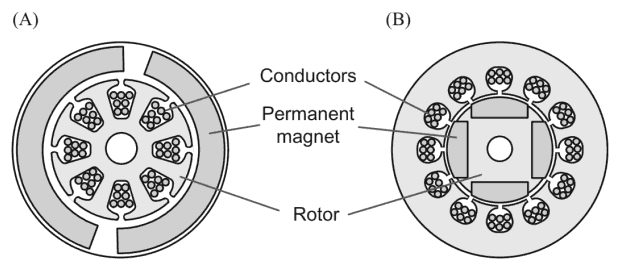
\includegraphics[width=8cm]{imagens/Comparativo.png}
	\legendafonte{\cite{kim2017electric}.}
 \label{fig:motor-dc-bldc-comparativo}
\end{figure}

Apesar das muitas vantagens, eles não estão isentos de algumas limitações. A complexidade eletrônica necessária para o controle preciso, o custo inicial potencialmente mais elevado comparado a motores elétricos escovados, a sensibilidade a ambientes de alta temperatura, pois podem gerar a desmagnetização dos imãs permanentes, a exigência de eletrônica de controle especializada, o potencial de ruído eletromagnético (EMI) e a complexidade de manutenção do sistema como um todo são fatores a serem considerados ao escolher essa tecnologia. Cada aplicação específica deve ponderar essas considerações em relação aos benefícios que os BLDC oferecem, como rendimento, durabilidade e controle superior.

São categorizados como síncronos, ou seja, o rotor gira na mesma frequência do campo magnético gerado pelo estator \cite{jahns1984torque}. Também não apresentam o fenômeno de escorregamento que é característico dos motores de indução. Os motores BLDC estão disponíveis em configurações de uma fase, duas fases e três fases, sendo  essa a mais amplamente utilizada, por serem equilibrados em relação a oscilação de torque e custo de construção \cite{hendershot1994design}.

A nomenclatura "Brushless DC" pode gerar uma interpretação equivocada. Embora alimentado por uma fonte de corrente contínua (DC), o motor BLDC é, em sua essência, um motor síncrono de ímãs permanentes (PMSM) \parencite{maquinasEletricasFitzgerald}. A rotação é induzida por campos magnéticos girantes gerados nos enrolamentos do estator, que são alimentados por formas de onda de corrente alternada (AC) sintetizadas por um controlador eletrônico. Portanto, a designação "DC" refere-se à fonte de alimentação externa, e não ao princípio físico de operação interna, que requer uma lógica de controle sofisticada para operar \parencite{ti2013sensorless}.

Nesse contexto, a performance do sistema é governada por parâmetros intrínsecos que descrevem a física da conversão de energia. Duas das mais importantes dessas constantes são a \textbf{constante de torque ($K_T$)} e a \textbf{constante de velocidade ($K_V$)}. Estes parâmetros são a manifestação matemática dos princípios físicos que regem a interação entre os domínios elétrico e mecânico do motor.

\subsection{Fundamentos Físicos da Conversão Eletromecânica}

A operação de um motor elétrico é governada por dois princípios físicos interligados: a Força de Lorentz, que gera o torque, e a Lei da Indução de Faraday, que gera uma força contraeletromotriz.

\subsubsection{A Força de Lorentz e a Condição de Torque Máximo}

A produção de força mecânica em um motor origina-se na Força de Lorentz. Esta lei descreve a força ($\vec{F}$) sobre um condutor de comprimento vetorial ($\vec{L}$) percorrido por uma corrente ($I$) e imerso em um campo magnético ($\vec{B}$). A relação vetorial é:
\begin{equation}
    \vec{F} = I \cdot (\vec{L} \times \vec{B})
\end{equation}
A magnitude desta força, $F = I \cdot L \cdot B \cdot \sin(\theta)$, onde $\theta$ é o ângulo entre o condutor e o campo magnético, é maximizada quando $\sin(\theta) = 1$, o que ocorre precisamente quando $\theta = 90^{\circ}$. Esta condição de ortogonalidade é o princípio mais elementar para a máxima conversão de energia.

Em um motor rotativo, o objetivo é o torque, que pode ser entendido como a interação entre o campo magnético gerado pelo estator ($\vec{B}_{\text{estator}}$) e o campo gerado pelos ímãs permanentes do rotor ($\vec{B}_{\text{rotor}}$). O torque eletromagnético ($\vec{T}_{em}$) é o produto vetorial desses dois campos \cite{vas1998vector}:
\begin{equation}
    \vec{T}_{em} \propto \vec{B}_{\text{estator}} \times \vec{B}_{\text{rotor}}
\end{equation}
A magnitude do torque é, portanto, diretamente proporcional ao seno do ângulo elétrico ($\theta_e$) entre os dois vetores de campo. O torque máximo é alcançado quando este ângulo é mantido em 90 graus elétricos. Manter esta condição de ortogonalidade de forma contínua é o objetivo central das estratégias de controle de alto desempenho, como o Controle Orientado por Campo (FOC), pois garante não apenas o torque máximo para uma dada corrente, mas também o máximo rendimento na conversão eletromecânica.

\subsubsection{A Lei de Faraday}
Simultaneamente à produção de torque, um motor em rotação atua como um gerador. A Lei da Indução de Faraday afirma que a variação do fluxo magnético através de uma espira de fio induz uma força eletromotriz (FEM). Em um motor, o movimento dos ímãs do rotor em relação aos enrolamentos do estator induz uma tensão conhecida como \textbf{força contraeletromotriz (FCEM)}, ou \textit{back-EMF}.

De acordo com a Lei de Lenz, a polaridade desta tensão induzida ($e_a$) se opõe diretamente à tensão terminal ($V$) aplicada ao motor \parencite{infineon2011bldc}. A magnitude da FCEM é diretamente proporcional à velocidade angular ($\omega$) do motor, estabelecendo a ligação física entre o movimento mecânico (velocidade) e um fenômeno elétrico (tensão induzida).

\subsection{Modelo Matemático do Motor e a Definição das Constantes}

Os princípios de Lorentz e Faraday são sintetizados em um modelo matemático que descreve a dinâmica do motor.

\textbf{Equação Elétrica (Lei de Kirchhoff):}
\begin{equation}
    V = e_a + I_a \cdot R_a + L_a \cdot \frac{dI_a}{dt}
\end{equation}
Onde $V$ é a tensão aplicada, $e_a$ é a FCEM de Armadura, $I_a \cdot R_a$ é a queda de tensão resistiva de Armadura e $L_a \cdot \frac{dI_a}{dt}$ é a queda de tensão indutiva de Armadura \parencite{maquinasEletricasFitzgerald}. Vale ressaltar que Armadura é o termo técnico para o enrolamento em motores elétricos, onde a principal conversão de energia acontece.

\textbf{Equação Mecânica (2ª Lei de Newton para Rotação):}
\begin{equation}
    T_e = T_l + J \cdot \frac{d\omega}{dt} + B \cdot \omega
\end{equation}
Onde $T_e$ é o torque eletromagnético, $T_l$ é o torque de carga, $J \cdot \frac{d\omega}{dt}$ é o torque inercial e $B \cdot \omega$ é o torque de atrito viscoso \parencite{maquinasEletricasFitzgerald}.

Dentro deste modelo, as constantes do motor surgem como os fatores de proporcionalidade que conectam os domínios elétrico e mecânico.

\subsection{\texorpdfstring{A constante de Torque $K_T$}{A constante de Torque KT}}
\label{KT}
A constante de torque ($K_T$) define a capacidade de um motor de converter corrente elétrica em torque mecânico. É formalmente definida como a relação linear:
\begin{equation}
    T_e = K_T \cdot I_a
\end{equation}
O valor de $K_T$ não é arbitrário, mas determinado pelas características construtivas do motor \parencite{hendershot1994design}:
\begin{itemize}
    \item \textbf{Força do Campo Magnético ($B$):} Ímãs mais fortes (ex: Neodímio) resultam em um $K_T$ maior.
    \item \textbf{Configuração do Enrolamento:} É diretamente proporcional ao número de espiras ($N$) nos enrolamentos.
    \item \textbf{Geometria do Motor:} Dimensões como o comprimento e o raio do estator influenciam diretamente seu valor.
\end{itemize}
Para um dado torque de carga, um motor com $K_T$ maior demandará uma corrente menor, resultando em menores perdas por efeito Joule ($P = I^2 \cdot R$) e, portanto, maior rendimento.

\subsection{\texorpdfstring{As constantes de Velocidade $K_V$}{As constantes de Velocidade KV}}
\label{KV}

De forma análoga, a relação entre a FCEM e a velocidade é quantificada por constantes.
\begin{itemize}
    \item \textbf{Constante de FCEM ($K_e$):} É a constante física que relaciona a FCEM gerada ($e_a$) com a velocidade angular do motor ($\omega$):
    \begin{equation}
        e_a = K_e \cdot \omega
    \end{equation}
    Assim como $K_T$, $K_e$ (também denotado como $k_b$) depende do projeto físico do motor \parencite{zoltan2012understanding}.

    \item \textbf{Constante de Velocidade ($K_V$):} Muito mais comum em folhas de dados comerciais, $K_V$ é definida como a relação entre a velocidade do motor sem carga e a tensão aplicada, geralmente em unidades de \textbf{RPM/V}. A relação entre $K_V$ e $K_e$ é de simples inversão \parencite{infineon2011bldc}:
    \begin{equation}
        K_V = \frac{1}{K_e}
    \end{equation}
    A FCEM é o mecanismo que limita a velocidade máxima do motor. O motor acelera até que a FCEM ($e_a = K_e \cdot \omega$) se aproxime da tensão de alimentação ($V$), ponto no qual a corrente resultante é apenas suficiente para vencer o atrito.
\end{itemize}

\subsection{\texorpdfstring{A Equivalência entre $K_T$ e $K_e$}{A Equivalência entre KT e Ke}}

Um dos resultados mais notáveis na teoria de motores é a equivalência numérica entre $K_T$ e $K_e$ quando ambas são expressas em unidades do Sistema Internacional (SI): \textbf{Nm/A} para $K_T$ e \textbf{V·s/rad} para $K_e$.
\begin{equation}
    K_T \text{ [Nm/A]} = K_e \text{ [V·s/rad]}
\end{equation}
Esta equivalência não é uma coincidência, mas uma consequência da \textbf{lei da conservação de energia}.

\textbf{Demonstração por Balanço de Potência:}
\begin{enumerate}
    \item A potência elétrica convertida em potência mecânica ($P_{\text{conv}}$) é a parte da potência de entrada que não é perdida como calor nos enrolamentos.

    \item A potência elétrica fornecida à armadura é
    \begin{equation}
        P_{\text{in}} = V \cdot I_a
    \end{equation}
    Substituindo a equação elétrica $V = e_a + I_a R_a$:
    \begin{equation}
        P_{\text{in}} = (e_a + I_a R_a) I_a = e_a I_a + I_a^2 R_a
    \end{equation}
    A parcela $I_a^2 R_a$ corresponde às perdas Joule nos enrolamentos; descontando-as, a potência eletromecanicamente convertida é
    \begin{equation}
        P_{\text{conv}} = e_a I_a
    \end{equation}

    \item A potência mecânica de saída ($P_{\text{mec}}$) é o produto do torque eletromagnético e da velocidade angular:
    \begin{equation}
        P_{\text{mec}} = T_e \cdot \omega
    \end{equation}

    \item Pela conservação de energia, a potência convertida iguala-se à potência mecânica de saída:
    \begin{equation}
        P_{\text{conv}} = P_{\text{mec}}
    \end{equation}

    \item Combinando os itens anteriores, $P_{\text{conv}} = P_{\text{mec}}$ implica
    \begin{equation}
        e_a I_a = T_e \omega
    \end{equation}
    Substituindo as definições $e_a = K_e \omega$ e $T_e = K_T I_a$:
    \begin{equation}
        (K_e \omega) I_a = (K_T I_a) \omega
    \end{equation}

    \item Para qualquer condição de operação não nula, podemos cancelar $\omega$ e $I_a$ de ambos os lados, provando que:
    \begin{equation}
        K_e = K_T
    \end{equation}
\end{enumerate}
Esta prova revela que o mesmo mecanismo de acoplamento eletromagnético que produz torque a partir da corrente (princípio motor, $K_T$) é o que gera tensão a partir do movimento (princípio gerador, $K_e$). Eles são duas manifestações do mesmo fenômeno físico \parencite{zoltan2012understanding, garcia1997modelagem}.

\subsection{Conversão de Unidades}

A elegância teórica é frequentemente obscurecida pelo uso de unidades inconsistentes na prática. A habilidade de converter valores de folhas de dados para o padrão SI é indispensável. A relação prática mais importante é entre $K_T$ e $K_V$:
\begin{equation}
    K_T \text{ [N·m/A]} = \frac{60 \cdot K_V \text{ [RPM/V]}}{2\pi}
\end{equation}
Esta fórmula é derivada diretamente da equivalência $K_T = K_e = 1/K_V$ após a conversão da velocidade para rad/s \parencite{infineon2011bldc}. A tabela abaixo resume as conversões chave.

\begin{table}[htbp]
\centering
\caption{Unidades de Constantes de Motor e Fatores de Conversão para o SI}
\label{tab:unidades}

\resizebox{\textwidth}{!}{%
\begin{tabular}{llll}
\toprule
\textbf{Parâmetro} & \textbf{Unidade SI} & \textbf{Unidades Comuns Não-SI} & \textbf{Fórmula de Conversão para SI} \\
\midrule
\textbf{Constante de Torque ($K_T$)} & N·m/A & oz-in/A & 1 oz-in/A = 0.00706155 N·m/A \\
 & & mN·m/A & 1 mN·m/A = 0.001 N·m/A \\
\addlinespace
\textbf{Constante de FCEM ($K_e$)} & V·s/rad & V/krpm & 1 V/krpm = 0.009549 V·s/rad \\
\addlinespace
\textbf{Constante de Velocidade ($K_V$)} & rad/(V·s) & RPM/V & 1 RPM/V = 0.10472 rad/(V·s) \\
\bottomrule
\end{tabular}%
}
\legendafonte{Elaborado pelo autor (2026).}
\end{table}

\subsection{\texorpdfstring{A Constante do Motor ($K_m$) como Figura de Mérito}{A Constante do Motor (Km) como Figura de Mérito}}

Uma constante mais fundamental para avaliar a qualidade do projeto de um motor é a \textbf{constante do motor ($K_m$)}:
\begin{equation}
    K_m = \frac{K_T}{\sqrt{R_a}}
\end{equation}
Sua unidade no SI é \textbf{N·m/$\sqrt{\text{W}}$}. $K_m$ representa a capacidade do motor de produzir torque por watt de potência dissipada como calor. Um $K_m$ mais alto indica um motor com maior rendimento na conversão de energia. Notavelmente, $K_m$ é invariante a alterações no enrolamento para um mesmo tamanho de carcaça, tornando-se uma excelente figura de mérito para comparar a qualidade de diferentes projetos de motores \parencite{infineon2011bldc}.

\subsection{Influência da Temperatura}

Embora chamadas de "constantes", $K_T$ e $K_e$ são afetadas pela temperatura. O aquecimento do motor causa uma redução na força magnética dos ímãs permanentes. Como ambas as constantes são diretamente proporcionais à densidade de fluxo magnético, um motor operando em alta temperatura produzirá menos torque para a mesma corrente (menor $K_T$) e precisará girar mais rápido para gerar a mesma FCEM (menor $K_e$, consequentemente um $K_V$ ligeiramente maior), resultando em uma performance geral degradada.

\section{Controlador Eletrônico de Velocidade (ESC)} 
 Os controladores eletrônicos de velocidade, são dispositivos eletrônicos que controlam a velocidade e o torque de motores BLDC. São classificados pela sua corrente e tensão máxima de saída. São constituídos dos seguintes componentes básicos: 

 \begin{itemize} 
 \item Circuito de entrada: O circuito de entrada converte a tensão fornecida pela bateria em tensão que pode ser usada pelo circuito de controle utilizando PWM para gerar uma tensão média desejada que será fornecida ao motor. Também pode inverter a sequência de comutação das fases fazendo com que o sentido de rotação também seja invertido. 
 \item Circuito de controle: O circuito de controle é responsável por calcular a corrente que deve ser fornecida às bobinas do motor. Normalmente se utilizam de sinais com características de PWM como sinal de referência para definir a velocidade e sentido de rotação. 
 \item Circuito de saída: O circuito de saída fornece a corrente necessária às bobinas do motor. 
 \end{itemize} 

 Além desses componentes básicos, os ESCs para motor BLDC pode incluir os seguintes recursos, além dos já discutidos anteriormente: 

 \begin{itemize} 
 \item Filtro de ruído: O filtro de ruído é usado para reduzir o ruído elétrico que pode ser gerado pelo motor. 
 \item Proteção térmica: A proteção térmica é usada para proteger o motor de superaquecimento. 
 \item Proteção contra sobrecarga: O ESC pode desligar o motor se ele experimentar correntes superiores às nominais que representam riscos de deterioração das bobinas do motor. 
 \end{itemize} 

  As equações lineares de um motor DC só são diretamente aplicáveis a um motor BLDC devido à ação sofisticada do seu \textbf{Controlador Eletrônico de Velocidade (ESC)}. O ESC realiza a comutação eletrônica, energizando sequencialmente os enrolamentos do estator para criar um campo magnético giratório. Isso força a complexa máquina AC a se comportar como o motor DC idealizado, tornando as constantes $K_T$ e $K_e$ ferramentas de análise e projeto perfeitamente válidas \parencite{hendershot1994design}.

 \subsection{\texorpdfstring{Consequências Práticas da Seleção de $K_V$}{Consequências Práticas da Seleção de KV}} 

 A seleção de $K_V$ é uma decisão de projeto crítica que estabelece um compromisso fundamental: 
 \begin{itemize} 
 \item \textbf{Motores de Alto $K_V$:} Possuem menos espiras de fio mais grosso. Resultam em baixo $K_T$, baixa resistência e baixa indutância. Para produzir torque, exigem alta corrente, mas atingem altas velocidades. Ideais para aplicações de alta velocidade e baixo torque, como drones de corrida e fusos de usinagem \parencite{tmotor2019kv}. 
 \item \textbf{Motores de Baixo $K_V$:} Possuem mais espiras de fio mais fino. Resultam em alto $K_T$, alta resistência e alta indutância. Geram alto torque com baixas correntes, apresentando maior rendimento para essa finalidade, mas com menor velocidade máxima. Ideais para aplicações de acionamento direto e alto torque, como drones de carga, guinchos e atuadores robóticos \parencite{byod2018kv}. 
 \end{itemize} 

 \subsection{Princípios de Operação} 

 O controlador eletrônico tem a função de fornecer tensão e corrente adequadas às bobinas do estator, visando o controle preciso da velocidade e do torque da máquina \cite{jahns1996pulsating}. A topologia fundamental para esta finalidade é a ponte inversora trifásica, à qual o motor BLDC pode ser acoplado em configuração estrela ou triângulo. O chaveamento dos transistores do inversor deve ser orquestrado de forma que cada fase seja percorrida por uma corrente com forma de onda senoidal ou trapezoidal. A excitação senoidal é voltada para um acionamento de alto desempenho e suavidade, enquanto a trapezoidal destaca-se pela simplicidade de controle e baixo custo de implementação. Para garantir a geração de um campo magnético girante e a rotação contínua do rotor, as formas de onda das três fases devem ser defasadas em 120 graus elétricos entre si.

 \subsubsection{Comutação de Seis Passos} 

 A comutação de seis passos demanda um sincronismo de disparo dos transistores de modo que, no modelo ideal, sempre dois deles estejam fechados: um transistor do lado superior (\textit{high-side}) conectado ao barramento positivo e um transistor do lado inferior (\textit{low-side}) conectado ao barramento negativo. Assim, em cada setor de $60^\circ$ elétricos, duas fases são energizadas e a terceira permanece eletricamente aberta para que sua FCEM possa ser observada (Figura \ref{fig:sequencia-acionamento-bldc}). Cada transistor permanece em condução durante $120^\circ$ elétricos.

 A denominação ``seis passos'', entretanto, descreve apenas os seis estados estacionários comandados pelo controlador ao longo de um ciclo elétrico. Do ponto de vista físico da corrente, cada passagem entre dois setores contém também um intervalo transitório de comutação. Portanto, uma descrição mais completa pode ser entendida como doze subintervalos por ciclo elétrico: seis intervalos de condução principal, nos quais a corrente percorre duas fases, e seis intervalos de transferência, nos quais a corrente da fase que está sendo desligada ainda precisa encontrar um caminho de circulação.

 Esse comportamento ocorre porque os enrolamentos do estator são indutivos. A corrente de uma indutância não pode variar instantaneamente; logo, quando um MOSFET é bloqueado, a corrente que circulava naquela fase não desaparece. Ela força a tensão do terminal da fase a se deslocar até polarizar diretamente o diodo de corpo de algum MOSFET da ponte, ou o próprio MOSFET complementar quando há retificação síncrona. A corrente que estava circulando pela fase de saída continua fluindo pela indutância da fase de saída e é desviada para um caminho de roda livre formado pelos diodos intrínsecos dos MOSFETs, pelo barramento CC e pelos capacitores do \textit{DC link}, até que sua energia magnética seja transferida, dissipada nas resistências do circuito ou devolvida temporariamente ao barramento.

 Considere, por exemplo, a transição do setor $A^+B^-$ para o setor $A^+C^-$. Antes da comutação, a corrente principal percorre o caminho $+V_{DC} \rightarrow H_A \rightarrow A \rightarrow B \rightarrow L_B \rightarrow -V_{DC}$, onde $H_A$ representa o transistor superior da fase A e $L_B$ o transistor inferior da fase B. Quando $L_B$ é desligado, a corrente que saía pela fase B continua no mesmo sentido por causa da energia armazenada na indutância. Como o caminho pelo transistor inferior foi aberto, o terminal B é elevado até conduzir pelo diodo de corpo do transistor superior da mesma fase ($H_B$), fechando uma malha de recirculação que passa pelo barramento positivo. Ao mesmo tempo, $L_C$ começa a conduzir e a corrente cresce na nova fase de retorno C. Durante esse intervalo, a corrente se divide entre uma malha antiga em decaimento, associada à fase B, e uma malha nova em crescimento, associada à fase C.

 O caso complementar ocorre quando a fase que está saindo era a fase conectada ao barramento positivo. Em uma transição como $A^+C^-$ para $B^+C^-$, o transistor superior de A é bloqueado e a corrente da fase A, que ainda tende a entrar no enrolamento, força o terminal A a conduzir pelo diodo de corpo do transistor inferior de A ($L_A$). Assim, quando a fase de saída era um caminho de \textit{source}, a corrente é desviada para o barramento negativo; quando a fase de saída era um caminho de \textit{sink}, a corrente é desviada para o barramento positivo. A Tabela \ref{tab:subintervalos_comutacao_6step} resume essa sequência para uma rotação elétrica completa.

\begin{table}[htbp]
\centering
\caption{Estados principais e intervalos transitórios na comutação trapezoidal}
\label{tab:subintervalos_comutacao_6step}
\small
\begin{tabular}{@{}p{1.5cm}p{2.2cm}p{4.3cm}p{5.1cm}@{}}
\toprule
Setor & Estado principal & Caminho principal da corrente & Intervalo de transferência para o próximo setor \\
\midrule
1 & $A^+B^-$ & $+V_{DC} \rightarrow H_A \rightarrow A \rightarrow B \rightarrow L_B \rightarrow -V_{DC}$ & $B$ deixa de ser a fase de retorno; sua corrente decai pelo diodo de $H_B$, enquanto $C$ passa a conduzir por $L_C$. \\
2 & $A^+C^-$ & $+V_{DC} \rightarrow H_A \rightarrow A \rightarrow C \rightarrow L_C \rightarrow -V_{DC}$ & $A$ deixa de ser a fase de alimentação; sua corrente decai pelo diodo de $L_A$, enquanto $B$ passa a conduzir por $H_B$. \\
3 & $B^+C^-$ & $+V_{DC} \rightarrow H_B \rightarrow B \rightarrow C \rightarrow L_C \rightarrow -V_{DC}$ & $C$ deixa de ser a fase de retorno; sua corrente decai pelo diodo de $H_C$, enquanto $A$ passa a conduzir por $L_A$. \\
4 & $B^+A^-$ & $+V_{DC} \rightarrow H_B \rightarrow B \rightarrow A \rightarrow L_A \rightarrow -V_{DC}$ & $B$ deixa de ser a fase de alimentação; sua corrente decai pelo diodo de $L_B$, enquanto $C$ passa a conduzir por $H_C$. \\
5 & $C^+A^-$ & $+V_{DC} \rightarrow H_C \rightarrow C \rightarrow A \rightarrow L_A \rightarrow -V_{DC}$ & $A$ deixa de ser a fase de retorno; sua corrente decai pelo diodo de $H_A$, enquanto $B$ passa a conduzir por $L_B$. \\
6 & $C^+B^-$ & $+V_{DC} \rightarrow H_C \rightarrow C \rightarrow B \rightarrow L_B \rightarrow -V_{DC}$ & $C$ deixa de ser a fase de alimentação; sua corrente decai pelo diodo de $L_C$, enquanto $A$ passa a conduzir por $H_A$. \\
\bottomrule
\end{tabular}
\end{table}

 Dessa forma, o controle é comandado em seis setores, mas a corrente percorre doze situações relevantes: seis caminhos principais de produção de torque e seis caminhos transitórios de roda livre ou regeneração parcial. Durante essas transições, nenhuma fase é instantaneamente desligada em termos eletromagnéticos; a fase de saída permanece conduzindo por diodo por uma fração do período, enquanto a fase de entrada ainda está estabelecendo corrente. A consequente distorção transitória das tensões de fase e a assimetria entre a corrente que decai e a corrente que cresce são as principais causas das oscilações no torque do motor (\textit{torque ripple}) características deste método \cite{kim2017electric, jahns1996pulsating}.
 
 Esse algoritmo de acionamento dos transistores, também chamado de Controle Trapezoidal, é a base para o funcionamento do motor BLDC. Embora seja possível operá-lo em malha aberta (sequência fixa), esta abordagem apresenta baixo rendimento e é propensa à perda de sincronismo sob variações de carga. Portanto, neste trabalho, projeta-se e implementa-se a infraestrutura de \textit{hardware} e \textit{firmware} para um \textbf{ESC trapezoidal \textit{sensorless}}, incluindo os circuitos de reconstrução de neutro virtual, filtragem RC e comparadores LM339 destinados à detecção de cruzamento por zero (ZCD) da FCEM. 
 
 \begin{figure}[htbp]
    \centering
    \caption{Sequência de acionamento para um BLDC trifásico.}
    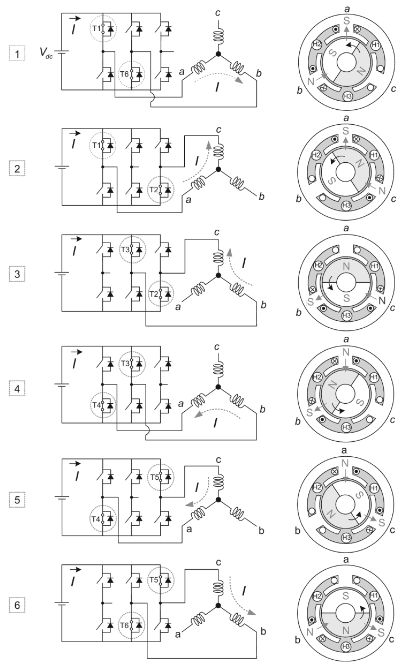
\includegraphics[width=11cm]{imagens/acionamento.png}
    \legendafonte{\cite{kim2017electric}.}
    \label{fig:sequencia-acionamento-bldc}
\end{figure}

 Nesta etapa de validação, a comutação opera em \textbf{malha aberta} (alinhamento e rampa forçada); a \textbf{transição para comutação em malha fechada orientada por ZCD} permanece como passo subsequente, após a confirmação da sequência 6-step e do condicionamento do sinal, conforme detalhado no Capítulo 4.

 Quando a aplicação necessita que o motor possua apenas uma velocidade, a fonte de alimentação de tensão fixa é suficiente. Para casos onde é necessário variar a velocidade do motor, a técnica de Modulação por Largura de Pulso (PWM) é normalmente empregada. Um ESC, por exemplo, utiliza PWM para ajustar a tensão média aplicada ao motor, controlando assim sua velocidade. Essa técnica, no entanto, pode demandar a utilização de controladores que comparem a velocidade desejada com a medida no rotor para um controle preciso, estratégia desenvolvida teoricamente na Seção~\ref{sec:controle_pi}. 

 \subsubsection{Análise da Ondulação de Torque (Torque Ripple)}
A principal desvantagem intrínseca à comutação forçada de seis passos (malha aberta) é a geração de uma ondulação de torque (\textit{torque ripple}), que se manifesta como pulsações no torque de saída do motor \cite{jahns1984torque, ali2017implementation}. Essas pulsações podem causar oscilações na velocidade, ruído acústico e vibrações mecânicas, sendo particularmente prejudiciais em aplicações que exigem alta precisão de movimento \cite{jahns1996pulsating}. A frequência desta ondulação é seis vezes a frequência elétrica fundamental do motor, correspondendo a uma pulsação a cada evento de comutação \cite{jahns1984torque}. Conforme analisado em trabalhos seminais como os de Jahns (1984) e Hendershot \& Miller (1994), este fenômeno é consequência de dois fatores principais \cite{kim2017electric, hendershot1994design}.

\begin{enumerate}
    \item \textbf{Incompatibilidade de Formas de Onda:} O modelo ideal do controle trapezoidal assume uma forma de onda de corrente perfeitamente retangular e uma FCEM perfeitamente trapezoidal. Na prática, a FCEM dos motores reais raramente é um trapézio ideal, e a corrente injetada não é perfeitamente retangular. Qualquer desalinhamento ou incompatibilidade entre a forma de onda da corrente e a da FCEM resulta em variações no torque produzido, conforme a equação $T_{e} = (e_{a} \cdot i_{a} + e_{b} \cdot i_{b} + e_{c} \cdot i_{c}) / \omega$ \cite{hendershot1994design}.

    \item \textbf{Transientes de Comutação:} A causa mais significativa da ondulação de torque é o próprio processo de comutação. Devido à indutância presente nos enrolamentos do motor, a corrente não pode variar instantaneamente. Quando o controlador comuta de um passo para o outro (por exemplo, de A-B para A-C), há um período de tempo finito durante o qual a corrente na fase que está sendo desligada (fase B) decai através do diodo de roda livre, e a corrente na fase que está sendo ligada (fase C) aumenta através da chave ativa \cite{jahns1996pulsating, joice2013compensation}. Durante este intervalo de comutação, o torque eletromagnético total produzido pelo motor não é constante. A taxa de variação da corrente na fase de entrada ($\frac{di_{in}}{dt}$) e na de saída ($\frac{di_{out}}{dt}$) é assimétrica devido à diferença de potencial aplicada em cada malha. Enquanto o crescimento da corrente na fase de entrada é retardado pela oposição da sua Força Contra-Eletromotriz (FCEM), o decaimento da corrente na fase de saída é acelerado pela soma da tensão do barramento com a sua respectiva FCEM durante a condução pelo diodo de roda livre. Essa diferença nas derivadas de corrente gera uma perturbação transitória na soma total das correntes do estator, resultando em um mergulho (\textit{dip}) ou pico de torque a cada $60^{\circ}$ elétricos \cite{choi1998commutation, chen2019commutation}.

\end{enumerate}

A ondulação de torque não é apenas um efeito colateral indesejado; é a manifestação mecânica de uma conversão de energia eletromecânica periodicamente de baixo rendimento. O objetivo do motor é converter potência elétrica em potência mecânica (torque vezes velocidade) de forma contínua e suave. Durante os intervalos de comutação, o vetor de corrente do estator está em transição entre duas posições estáveis. Neste período, o alinhamento entre o campo magnético do estator e o campo magnético do rotor desvia-se momentaneamente da orientação ótima de $90^{\circ}$ elétricos necessária para a produção máxima de torque. Consequentemente, para uma mesma magnitude de corrente de entrada, o torque de saída é reduzido, representando uma queda transitória no rendimento da conversão de energia. A ondulação de torque observada é, portanto, o resultado direto desses intervalos de conversão sub-ótima, inerentes à natureza discreta do chaveamento de seis passos.

\subsubsection{Modulação por Largura de Pulso (PWM)} 

O controle de velocidade e torque de motores BLDC exige a imposição de uma tensão terminal variável nos enrolamentos do estator. Dado que as fontes de alimentação primárias disponíveis na maioria das aplicações (como baterias e fontes de bancada) operam com uma tensão contínua fixa ($V_{DC}$), faz-se necessária a aplicação da técnica de Modulação por Largura de Pulso (PWM, \textit{Pulse Width Modulation}). Esta técnica consiste no chaveamento periódico de alta frequência dos semicondutores de potência da ponte inversora, aplicando pulsos de tensão retangulares de amplitude fixa e largura variável à carga indutiva.

O parâmetro fundamental que rege o comportamento do PWM é a razão cíclica (\textit{duty cycle}, $D$), definida matematicamente como a relação entre o tempo em que o sinal permanece em nível lógico alto ($t_{on}$) e o período total do ciclo de chaveamento ($T$), conforme expresso na Equação \ref{eq:duty_cycle}:

\begin{equation}
D = \frac{t_{on}}{T} = t_{on} \cdot f_c
\label{eq:duty_cycle}
\end{equation}

Em que $f_c$ representa a frequência de portadora ou frequência de chaveamento. A tensão média efetiva entregue aos enrolamentos do estator ($V_{m\text{é}dia}$) é obtida por meio da integração do sinal de tensão instantâneo ao longo de um período completo, resultando em uma relação linear direta com a razão cíclica, explicitada na Equação \ref{eq:v_media}:

\begin{equation}
V_{m\text{é}dia} = \frac{1}{T} \int_{0}^{t_{on}} V_{DC} \, dt = \frac{t_{on}}{T} V_{DC} = D \cdot V_{DC}
\label{eq:v_media}
\end{equation}

A seleção da frequência de chaveamento ($f_c$) constitui um compromisso crítico de projeto de engenharia, governado por restrições de ordem magnética, acústica e térmica. Motores BLDC de alto desempenho e tamanho reduzido comumente apresentam resistência estatórica e indutância de fase extremamente baixas. Sob frequências de chaveamento reduzidas, a baixa constante de tempo indutiva ($\tau = L/R$) resulta em uma elevada ondulação de corrente (\textit{current ripple}), o que culmina em perdas excessivas por efeito Joule no cobre e geração de ruído acústico na faixa audível humana (20 Hz a 20 kHz). 

Por outro lado, a elevação excessiva de $f_c$ acarreta o aumento linear das perdas por comutação (\textit{switching losses}) nos MOSFETs de potência, dadas pela transição periódica entre os estados de condução e bloqueio, conforme modelado simplificadamente na Equação \ref{eq:perdas_comutacao}:

\begin{equation}
P_{sw} = V_{DC} \cdot I_{out} \cdot f_c \cdot \left( \frac{t_r + t_f}{2} \right)
\label{eq:perdas_comutacao}
\end{equation}

Em que $I_{out}$ é a corrente de saída, e $t_r$ e $t_f$ são os tempos de subida (\textit{rise time}) e descida (\textit{fall time}) do transistor, respectivamente. No desenvolvimento de inversores voltados a protótipos de ESC, adota-se rotineiramente uma frequência de portadora de aproximadamente 20 kHz. Esse valor se posiciona no limiar superior da audição humana, mitigando poluição sonora decorrente do magnetostritismo, ao mesmo tempo em que preserva a integridade térmica dos transistores e minimiza a ondulação da corrente contínua através do estator.

No âmbito da comutação trapezoidal de seis passos, o sinal PWM gerado pelo periférico de controle (como o módulo MCPWM) pode ser aplicado de diferentes formas aos braços do inversor trifásico durante o setor de condução de $120^\circ$ elétricos. Destacam-se as seguintes estratégias de modulação unipolar:

\begin{itemize}
    \item \textbf{Estratégia H\_PWM - L\_ON:} O sinal PWM de alta frequência é aplicado exclusivamente ao transistor do lado da alta (\textit{High-Side}), enquanto o dispositivo correspondente do lado da baixa (\textit{Low-Side}) permanece permanentemente conduzindo em nível contínuo (SINK) durante todo o intervalo de $120^\circ$. Esta abordagem reduz sensivelmente as perdas por comutação totais da ponte, uma vez que apenas uma das chaves ativas sofre transições rápidas a cada período.
    \item \textbf{Estratégia H\_ON - L\_PWM:} Configuração inversa à anterior, na qual a chave superior é mantida saturada em nível lógico alto e a chave inferior modula a corrente em alta frequência.
\end{itemize}

Durante os períodos de desligamento do PWM ($t_{off}$) na estratégia H\_PWM - L\_ON, a energia armazenada no campo magnético indutivo da bobina força a circulação da corrente através do diodo de roda livre intrínseco do MOSFET complementar, estabelecendo um circuito de recirculação. A correta temporização e o entendimento de que a largura de pulso atua diretamente na magnetização do estator formam o alicerce para o controle de torque do sistema.

\begin{figure}[htbp]
    \centering
    \caption{Modulação por largura de pulso utilizando uma fonte de $100V$.}
    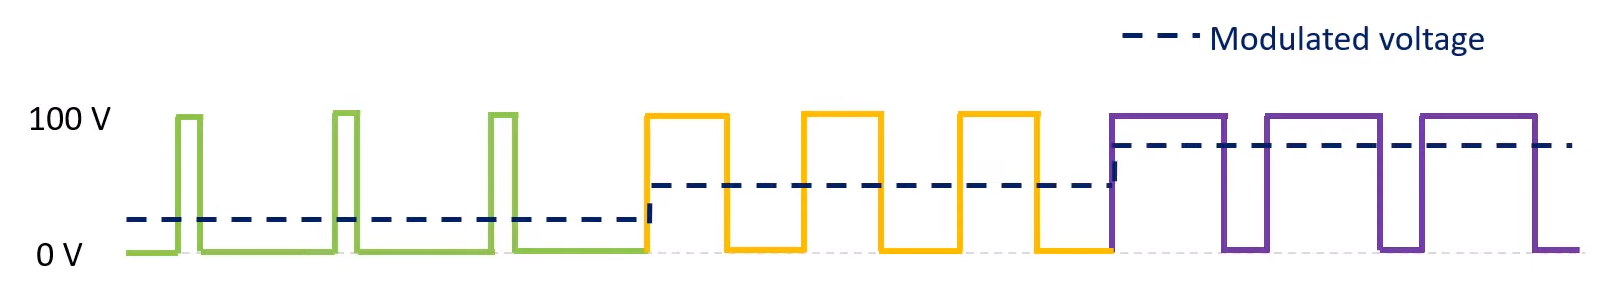
\includegraphics[width=0.85\textwidth]{imagens/PWM.png}
    \legendafonte{\cite{matlabBLDC}.}
    \label{fig:pwm-fonte-100v}
\end{figure}

 \subsection{Estratégia de Partida em Malha Aberta para Operação \textit{Sensorless}}

A implementação de um controle \textit{sensorless} eficaz depende da capacidade do controlador de estimar a posição do rotor a partir de grandezas elétricas, mais comumente a FCEM. Contudo, esta abordagem apresenta um desafio fundamental: em repouso (velocidade zero), não há movimento relativo entre os ímãs do rotor e os enrolamentos do estator, e, portanto, nenhuma FCEM é gerada \cite{ti2013sensorless, nxp2023sensorless}. Nesta condição "cega", o controlador não possui informações sobre a posição angular do rotor, tornando impossível determinar qual par de fases deve ser energizado para iniciar a rotação na direção desejada. Para superar essa limitação, é necessária uma rotina de partida especializada, operando em malha aberta, que força o motor a girar até que uma velocidade suficiente seja atingida para que a FCEM se torne detectável e o controle em malha fechada possa assumir. Este procedimento é universalmente dividido em duas fases sequenciais: alinhamento e comutação forçada.

\subsubsection{Alinhamento do Rotor}

O primeiro passo para uma partida confiável é estabelecer uma posição inicial conhecida para o rotor. A fase de alinhamento realiza isso ao energizar um conjunto específico de enrolamentos do estator com uma corrente contínua (DC) por um período de tempo pré-determinado \cite{ti2022minimizing, nxp2023sensorless}. Por exemplo, o controlador pode aplicar uma tensão positiva à fase C e conectar as fases A e B ao terra \cite{ti2022minimizing}. Esta ação cria um campo magnético estático e fixo no estator. Os ímãs permanentes do rotor, livres para girar, irão se alinhar com este campo para minimizar a relutância magnética do circuito, de forma análoga a uma agulha de bússola se alinhando com o campo magnético terrestre. Ao final deste processo, o rotor estará travado em uma posição angular conhecida e previsível. Os parâmetros críticos que governam esta fase são a duração do alinhamento e a magnitude da corrente de alinhamento \cite{ti2022minimizing}.

 A fase de alinhamento funciona como uma etapa de otimização pré-torque, o seu objetivo primordial é condicionar o sistema para que o primeiro passo de comutação dinâmica gere o máximo torque possível. O maior desafio ao iniciar um motor a partir do repouso é vencer a inércia da carga e o atrito estático, o que exige um impulso de torque inicial elevado. A teoria de motores elétricos, conforme estabelecido na Seção 1.1.1, dita que o torque é maximizado quando o campo magnético do estator está orientado a $90^{\circ}$ elétricos em relação ao campo do rotor. O algoritmo de controle é projetado sabendo a posição final do rotor após o alinhamento. Assim, a primeira combinação de fases a ser energizada na fase seguinte (rampa de aceleração) é escolhida para criar um novo vetor de campo magnético do estator que esteja precisamente na orientação ótima em relação à posição agora conhecida do rotor. Isso garante que o primeiro passo dinâmico produza um torque potente e eficaz, "chutando" o rotor para o movimento e superando as resistências iniciais. Uma duração de alinhamento insuficiente ou uma corrente muito baixa pode resultar em um alinhamento incompleto, levando a um torque inicial fraco e, consequentemente, a uma falha na partida \cite{ti2022minimizing}.

\subsubsection{Comutação Forçada (Rampa de Aceleração)}

Com o rotor devidamente alinhado, o controlador inicia a fase de comutação forçada. Nesta etapa, o sistema opera em malha aberta, comutando as fases em uma sequência predefinida, sem qualquer realimentação da posição do rotor \cite{nxp2023sensorless}. A frequência de comutação não é aplicada abruptamente; em vez disso, ela é aumentada gradualmente a partir de um valor inicial baixo, seguindo um perfil de aceleração pré-programado, conhecido como "curva de partida em malha aberta" (\textit{open-loop starting curve}) \cite{ti2022minimizing}. Esta rampa de aceleração é definida por coeficientes pré-definidos \cite{ti2022minimizing}.

Durante esta fase, o controlador essencialmente comanda a rotação do campo magnético do estator e "assume" que o rotor, devido à sua inércia e ao torque gerado, conseguirá acompanhar este campo giratório. O processo continua, com a frequência de comutação aumentando progressivamente, até que a velocidade de rotação do motor seja alta o suficiente (tipicamente em torno de $5\%$ da velocidade nominal) para que a FCEM gerada nos enrolamentos atinja uma amplitude que possa ser medida de forma confiável \cite{ti2022minimizing, nxp2023sensorless}. Neste ponto, o sistema realiza a transição (\textit{handoff}) do controle em malha aberta para um modo de controle em malha fechada (por exemplo, baseado na detecção de cruzamento por zero da FCEM), que é de maior rendimento e robusto para a operação contínua.

\subsection{Desafios e Limitações da Partida Forçada}

A estratégia de partida em malha aberta não é isenta de desafios e limitações significativas. A sua natureza "cega" a torna vulnerável a variações de carga e a parâmetros não ideais do sistema.

\subsubsection{Análise do Fenômeno de Perda de Sincronismo (Stall)}

O risco mais proeminente do controle em malha aberta é a perda de sincronismo, comumente conhecida como \textit{stall} ou perda de passo. Este fenômeno ocorre quando a aceleração real do rotor não consegue acompanhar a velocidade de rotação do campo magnético do estator imposta pelo controlador. Se o torque de carga aplicado ao eixo do motor, somado à sua própria inércia, for maior que o torque eletromagnético que o motor consegue produzir em um determinado passo, o rotor "perderá o passo" e ficará para trás \cite{nxp2023sensorless}. Isso pode ser causado por uma carga inicial muito elevada ou por uma rampa de aceleração excessivamente agressiva, que aumenta a frequência de comutação mais rápido do que o rotor consegue acelerar \cite{ti2022minimizing}.

Uma vez que o sincronismo é perdido, o alinhamento entre os campos do rotor e do estator se torna desfavorável, e a produção de torque efetivo colapsa. O resultado é um movimento errático, vibrações intensas, ruído audível e, frequentemente, a parada completa do motor, enquanto o controlador continua a injetar corrente nos enrolamentos de forma ineficaz. Este estado pode levar a picos de corrente perigosos para a eletrônica de potência. Por essa razão, o controle em malha aberta é inadequado para aplicações com cargas variáveis ou que exigem alto torque de partida.

\subsubsection{Outros Efeitos Adversos}

Além do risco de perda de passo, a partida forçada apresenta outras desvantagens:

\begin{itemize}
    \item \textbf{Picos de Corrente:} No início da partida, a velocidade do motor é baixa ou nula, o que significa que a FCEM, que normalmente se opõe à tensão de alimentação e limita a corrente, também é baixa ou inexistente. Sem essa oposição, a corrente que flui para os enrolamentos é limitada apenas pela resistência ôhmica e pela tensão aplicada, podendo atingir valores muito elevados se não for cuidadosamente controlada pelo \textit{duty cycle} do PWM. Estes picos de corrente podem estressar a bateria e os componentes da ponte inversora.
    \item \textbf{Vibração e Baixo Rendimento:} Como o controle é feito "às cegas", o alinhamento entre o campo do estator e o rotor durante a rampa de aceleração nunca é perfeito. Este desalinhamento constante é a fonte da ondulação de torque discutida anteriormente, que se manifesta como vibração mecânica e resulta em uma operação de baixo rendimento, onde uma parte da energia elétrica consumida é dissipada em vez de ser convertida em torque útil.
\end{itemize}

É fundamental reiterar que a partida forçada em malha aberta é uma fase transitória e um meio para um fim. É uma estratégia de \textit{bootstrap} projetada exclusivamente para levar o motor de um estado de repouso para uma velocidade operacional mínima, onde métodos de controle em malha fechada, de maior rendimento, precisos e robustos, podem ser ativados para a operação contínua do sistema \cite{ti2022minimizing, nxp2023sensorless}.

\section{Controle Proporcional-Integral em Malhas Fechadas de ESC}
\label{sec:controle_pi}

Além da comutação trapezoidal e da modulação PWM, a operação precisa de um ESC em regime depende de \textbf{malhas de realimentação} que ajustem continuamente a tensão média aplicada ao motor (ou a corrente de fase) de modo a acompanhar referências de corrente ou velocidade impostas pelo operador. Neste trabalho, essa função é desempenhada por controladores \textbf{proporcional-integral (PI)}, algoritmo amplamente adotado em acionamentos de motores BLDC e PMSM por combinar simplicidade de implementação, robustez frente a perturbações de carga e capacidade de eliminar erro estacionário \cite{krishnan2010permanent, xia2012permanent, kim2017electric}.

\subsection{Distinção entre Malhas de Comutação e Malhas PI}
\label{subsec:distincao_malhas}

Um ESC trifásico opera com \textbf{duas camadas de controle independentes}, que não devem ser confundidas. A primeira decide \textit{quando} comutar as fases (sincronismo angular com o rotor); a segunda decide \textit{quanto} esforço elétrico aplicar em cada passo (corrente ou velocidade desejada). A nomenclatura ``malha aberta'' e ``malha fechada'' aplica-se separadamente a cada camada, e não ao sistema como um todo.

\begin{table}[htbp]
\centering
\caption{Duas camadas de controle no ESC deste trabalho}
\label{tab:camadas_controle}
\resizebox{\textwidth}{!}{%
\begin{tabular}{p{3.2cm}p{4.8cm}p{3.2cm}p{3.8cm}}
\toprule
\textbf{Camada} & \textbf{Grandeza regulada} & \textbf{Realimentação} & \textbf{Estado neste projeto} \\
\midrule
Comutação 6-step & Instante de troca de fase (posição do rotor) & FCEM/ZCD ou temporizador & Malha \textbf{aberta} na validação atual (rampa por temporizador; ver Subseções anteriores deste capítulo) \\
Malha PI & Corrente de fase e/ou velocidade & INA240 + ADC1; intervalo entre passos & Malha \textbf{fechada} sempre que o PI está ativo \\
\bottomrule
\end{tabular}%
}
\legendafonte{Elaborado pelo autor (2026).}
\end{table}

Três esclarecimentos estruturam o uso desses termos ao longo deste trabalho:

\begin{enumerate}
    \item \textbf{O controlador PI é malha fechada, e não aberta.} Por definição, o PI exige comparar referência $r$ com medição $y$ (Equação~\ref{eq:pi_continuo} adiante). No firmware, a corrente de fase é medida pelos amplificadores INA240 e convertida pelo ADC1; no modo velocidade, a velocidade é estimada a partir do intervalo entre passos de comutação. Sem essa realimentação, não haveria erro $e = r - y$ nem termo integral, tratar-se-ia apenas de um \textit{duty cycle} fixo ou de uma rampa pré-programada, o que não caracteriza um regulador PI.
    \item \textbf{O sistema ESC como um todo não é inteiramente malha fechada.} Na fase de validação descrita neste trabalho, a comutação trapezoidal avança em \textbf{malha aberta}: a sequência 6-step progride por temporizador (rampa de frequência elétrica), sem usar o cruzamento por zero da FCEM para sincronizar o rotor. A infraestrutura de \textit{hardware} para comutação em malha fechada por ZCD (comparadores LM339, neutro virtual) está projetada, mas o \textit{handover} para essa modalidade permanece como etapa subsequente (Subseção anterior sobre comutação \textit{sensorless} e Capítulo de Resultados). Enquanto isso, as malhas PI de corrente e velocidade operam em paralelo, em malha fechada, regulando o esforço elétrico dentro de cada passo comutado.
    \item \textbf{Onde cada conceito é tratado neste texto.} A comutação e a partida em malha aberta alinhamento, rampa forçada, risco de \textit{stall} e transição futura para ZCD, são desenvolvidas na Seção anterior (Controlador Eletrônico de Velocidade). A presente seção trata exclusivamente das malhas PI em malha fechada (corrente e velocidade). A implementação no firmware, ganhos $K_p$ e $K_i$, e os resultados de bancada encontram-se nos Capítulos de Metodologia e de Resultados e Discussão.
\end{enumerate}

\subsection{Fundamentos do Controlador PI}

Em uma malha fechada, o controlador recebe uma \textbf{referência} $r$ (por exemplo, corrente ou velocidade desejada) e compara-a com a \textbf{medição} $y$ proveniente dos sensores. O \textbf{erro} instantâneo é definido como:
\begin{equation}
    e(t) = r - y(t)
\end{equation}
A ação de controle $u(t)$ combina uma resposta proporcional ao erro atual e uma resposta integral que acumula o erro ao longo do tempo:
\begin{equation}
    u(t) = K_p \, e(t) + K_i \int_0^t e(\tau) \, d\tau
    \label{eq:pi_continuo}
\end{equation}
onde $K_p$ é o ganho proporcional e $K_i$ o ganho integral. O termo proporcional confere resposta imediata a desvios; o termo integral corrige desvios persistentes, pois continua a agir enquanto $e(t) \neq 0$.

Em sistemas embarcados, a Equação~\ref{eq:pi_continuo} é implementada em tempo discreto com período de amostragem $T_s = \Delta t$. Adotando integração de Euler, a forma recorrente adotada neste projeto é:
\begin{equation}
    P_k = K_p \, e_k
    \label{eq:pi_p_discreto}
\end{equation}
\begin{equation}
    I_k = I_{k-1} + K_i \, e_k \, \Delta t
    \label{eq:pi_i_discreto}
\end{equation}
\begin{equation}
    u_k = \mathrm{clamp}(P_k + I_k,\; u_{min},\; u_{max})
    \label{eq:pi_saida}
\end{equation}
Quando a saída $u_k$ atinge os limites físicos do atuador (por exemplo, o teto de \textit{duty cycle} do PWM), o integrador pode continuar a acumular erro (\textit{windup}), provocando sobressinal ao sair da saturação. Por isso, impõe-se \textbf{anti-windup} por limitação (\textit{clamping}) do estado integral $I_k$ dentro de intervalos $[I_{min}, I_{max}]$, detalhes de implementação no firmware são apresentados nos Capítulos de Metodologia e de Resultados.

\subsection{Limitações do Controle Proporcional Puro}

Um controlador puramente proporcional ($u = K_p \cdot e$) reage instantaneamente ao erro, mas apresenta uma limitação estrutural: na presença de perturbações constantes ou de plantas com comportamento integrador, o sistema estabiliza com \textbf{erro estacionário} não nulo. Intuitivamente, um ganho $K_p$ finito exige um erro residual para produzir a ação de controle necessária ao equilíbrio.

No contexto de um ESC trapezoidal, essa limitação manifesta-se de forma concreta. Para manter uma corrente de fase constante $I_{cmd}$, o \textit{duty cycle} do PWM deve compensar não apenas a queda ôhmica nos enrolamentos, mas também a FCEM, cujo valor cresce linearmente com a velocidade ($e_a = K_e \cdot \omega$). À medida que o motor acelera ou a tensão do barramento decai, o duty necessário para o mesmo $I_{cmd}$ aumenta. Um controlador P puro, com ganho fixo, não possui mecanismo para ajustar esse \textit{offset} operacional: a corrente medida estabilizaria abaixo da referência. O termo integral supre exatamente essa lacuna, acumulando a ação necessária até anular o erro residual.

De forma análoga, na regulagem de velocidade, variações de carga mecânica (atrito, inércia da carga) exigem correntes distintas para manter a mesma velocidade. Sem integral, um controlador P de velocidade deixaria um desvio permanente entre a referência e a rotação medida sempre que a carga se alterasse.

\subsection{Exclusão do Termo Derivativo: por que PI e não PID}

O controlador PID acrescenta um termo derivativo $K_d \cdot de/dt$, sensível à taxa de variação do erro. Embora possa melhorar a resposta transitória em plantas bem modeladas e pouco ruidosas, a inclusão do termo D neste ESC traz desvantagens que superam os benefícios esperados:

\begin{itemize}
    \item \textbf{Amplificação de ruído:} A corrente de fase é medida por amplificadores INA240 e convertida pelo ADC1 a $1\,\text{kHz}$, em ambiente de comutação PWM a $20\,\text{kHz}$ e de sequência trapezoidal de seis passos. O termo derivativo amplificaria as componentes de alta frequência (ripple de corrente, transientes de comutação), degradando a qualidade do sinal de realimentação e podendo induzir oscilações na saída do controlador.
    \item \textbf{Dinâmica dominante lenta:} A malha externa de velocidade e a sequência de comutação operam em escala de milissegundos (frequência elétrica de dezenas a centenas de hertz). A dinâmica mecânica e elétrica do sistema trapezoidal não se beneficia de previsão agressiva baseada em derivadas, ao contrário de malhas de corrente de FOC em dezenas de quilohertz.
    \item \textbf{Derivative kick:} Degraus na referência (comando do operador via gatilho analógico) produzem picos instantâneos em $de/dt$. Embora o firmware limite a taxa de variação da referência (\textit{slew rate limiter}), o termo D permaneceria sensível a saltos residuais de erro.
    \item \textbf{Prática consolidada:} Malhas de corrente e de velocidade em acionamentos BLDC trapezoidais utilizam PI como padrão industrial \cite{krishnan2010permanent, xia2012permanent, hanselman2003brushless}. A sintonia de três ganhos ($K_p$, $K_i$, $K_d$) com filtragem do termo derivativo agregaria complexidade sem retorno mensurável na arquitetura de controle adotada neste trabalho.
\end{itemize}

Por essas razões, o firmware deste projeto implementa estritamente controladores PI, sem termo derivativo.

\subsection{Aplicabilidade ao ESC Trifásico Deste Trabalho}

A estratégia de controle PI adapta-se diretamente à topologia do ESC desenvolvido, organizada em uma ou duas malhas conforme o modo operacional:

\begin{itemize}
    \item \textbf{Malha interna de corrente:} O PI de corrente compara a referência $I_{cmd}$ (limitada pelo operador ou pela malha externa) com a corrente de fase medida e produz o \textit{duty cycle} do PWM (0 a 95\,\%). Essa malha regula o esforço elétrico do motor, aproximando torque $\propto I$, e constitui a primeira linha de defesa contra sobrecorrente antes das proteções analógicas e de software.
    \item \textbf{Malha externa de velocidade (modo cascata):} Quando habilitado o modo de controle por velocidade, um segundo PI compara $RPM_{cmd}$ com a velocidade estimada a partir do intervalo entre passos de comutação 6-step e gera a referência de corrente para o PI interno. A corrente adapta-se automaticamente à carga mecânica, dentro do limite de 5\,A configurado.
    \item \textbf{Modo corrente direta:} Com apenas o PI de corrente ativo, a velocidade resultante depende da carga e da rampa de comutação em malha aberta, útil para ensaios de bancada com esforço elétrico limitado.
\end{itemize}

Dois requisitos de implementação derivam diretamente da teoria PI e condicionam o firmware: (1) o período de amostragem $\Delta t = 1\,\text{ms}$ deve ser estável, pois o termo integral da Equação~\ref{eq:pi_i_discreto} depende de $\Delta t$ constante, requisito tratado na Seção~\ref{sec:fundamentos_software}; (2) a saturação da saída em 95\,\% de \textit{duty cycle}, imposta pela recarga do capacitor de \textit{bootstrap} dos drivers IR2110, torna obrigatório o anti-windup para evitar sobressinal ao retornar da saturação.

A materialização dessas malhas no firmware, arquitetura em cascata, ganhos $K_p$ e $K_i$, temporizador de 1\,kHz e validação em bancada, é descrita no Capítulo de Metodologia e discutida no Capítulo de Resultados e Discussão.

\section{Aspectos de Eletrônica de Potência}

A implementação física do inversor exige a compreensão de componentes e técnicas que viabilizam a comutação em alta frequência e corrente.

\subsection{O MOSFET de Potência e Perdas}
O MOSFET (\textit{Metal-Oxide-Semiconductor Field-Effect Transistor}) é o dispositivo de chaveamento predominante em aplicações de baixa e média tensão devido à sua alta velocidade de comutação e facilidade de acionamento \cite{rashid2014power}. Em um inversor para controle de motores, o MOSFET não atua na região linear (amplificação), mas alterna entre os estados de corte (chave aberta) e saturação (chave fechada).

O rendimento do inversor é limitado por dois mecanismos principais de perda no MOSFET \cite{kim2017electric}:
\begin{itemize}
    \item \textbf{Perdas por Condução ($P_{cond}$):} Quando o transistor está ligado, ele apresenta uma resistência interna residual entre dreno e fonte, denominada $R_{DS(on)}$. A potência dissipada é dada por $P_{cond} = I_{D}^2 \cdot R_{DS(on)}$. Componentes modernos buscam minimizar o $R_{DS(on)}$ para reduzir o aquecimento.
    \item \textbf{Perdas por Comutação ($P_{sw}$):} Ocorrem durante a transição entre ligado e desligado. Como a tensão e a corrente não variam instantaneamente, há um breve período em que ambas são não-nulas, gerando um pico de potência dissipada. Esta perda é diretamente proporcional à frequência de chaveamento ($f_{sw}$) e à carga total de gate ($Q_g$) que o driver deve fornecer \cite{rashid2014power}.
\end{itemize}

\subsection{Seleção da Frequência de Chaveamento PWM}
\label{subsec:freq_chaveamento_pwm}

A frequência de chaveamento ($f_{sw}$) do PWM que modula os MOSFETs da ponte inversora é um parâmetro de projeto que acopla diretamente os mecanismos de perda descritos acima (em particular, $P_{sw} \propto f_{sw}$) à ondulação de corrente (\textit{ripple}) nas bobinas do motor e ao ruído acústico gerado por magnetostrição no estator \cite{mohan2003, hanselman2003brushless}. Não existe um valor universalmente ótimo: a indústria opera em faixas distintas conforme a aplicação, a dissipação térmica disponível no inversor e a carga de gate ($Q_g$) dos semicondutores selecionados \cite{rashid2014power}.

Neste trabalho adota-se \textbf{20 kHz} como compromisso de engenharia para o par MOSFET/driver IRFS7530--IR2110: a carga de gate elevada dos transistores automotivos selecionados torna inviável, com dissipação passiva no volume da placa, as faixas de alta performance do aeromodelismo (48 kHz ou 96 kHz, comuns em ESCs \textit{racing}), enquanto valores inferiores a 16 kHz reintroduziriam ruído audível. O dimensionamento quantitativo, perdas de comutação, \textit{ripple} de corrente e corrente média de \textit{gate} do driver, encontra-se na Subseção de Determinação da Frequência de Chaveamento do Capítulo de Metodologia.

\begin{table}[htbp]
    \centering
    \caption{Panorama de frequências de chaveamento PWM em acionamentos BLDC e afins}
    \label{tab:panorama_fsw_industria}
    \resizebox{\textwidth}{!}{%
    \begin{tabular}{lll}
    \toprule
    \textbf{Faixa típica} & \textbf{Segmento / aplicação} & \textbf{Característica principal} \\
    \midrule
    4--8 kHz & Drives industriais legados, ESCs de baixo custo & Audível; menores perdas de comutação \\
    8--12 kHz & Ferramentas elétricas, ESCs \textit{entry-level} & Zumbido perceptível ao operador \\
    16--24 kHz & ESCs BLDC genéricos, VANTs & Próximo ao limiar ultrassônico ($\approx 20\,\text{kHz}$) \\
    \textbf{20 kHz} & \textbf{Este projeto} & Equilíbrio térmico, silêncio e \textit{ripple} (Cap.~Metodologia) \\
    32--48 kHz & Aeromodelismo, \textit{drones} de consumo & Menor \textit{ripple}; $P_{sw}$ maior \\
    48--96 kHz & ESCs \textit{racing} (ex.: BLHeli, SimonK) & Alta resposta; exige baixo $Q_g$ e dissipação agressiva \\
    10--20 kHz+ & FOC industrial & Malha de corrente rápida; escopo distinto do trapezoidal 6-step \\
    \bottomrule
    \end{tabular}%
    }
    \legendafonte{Elaborado pelo autor (2026), com base em \cite{rashid2014power, hanselman2003brushless, mohan2003}.}
    \end{table}

\subsection{O Barramento DC e a Indutância Parasita}

Em inversores de fonte de tensão (VSI) que operam com altas frequências de chaveamento, a impedância da fonte de alimentação não pode ser considerada ideal. Os cabos de conexão entre a bateria e o inversor introduzem uma indutância parasita ($L_{par}$) significativa no circuito. Durante a comutação dos transistores, a rápida variação de corrente ($di/dt$) interage com essa indutância, gerando picos de tensão ($V_{spike}$) de acordo com a lei de Faraday-Lenz:

\begin{equation}
    V_{spike} = L_{par} \cdot \frac{di}{dt}
\end{equation}

Se não mitigados, esses picos podem superar a tensão de ruptura dos semicondutores, causando falhas catastróficas. Para solucionar esse problema, utiliza-se um banco de capacitores no barramento DC (\textit{DC Link}), posicionado fisicamente próximo aos interruptores. Este banco atua como uma fonte de tensão de baixa impedância local, fornecendo a corrente pulsada exigida pelo inversor e absorvendo a energia regenerada, além de filtrar a componente alternada (ripple) da corrente \cite{rashid2014power}.

Embora o cálculo analítico da capacitância mínima ($C_{min}$) seja classicamente derivado da máxima variação de tensão admissível ($\Delta V$) no barramento, conforme a Equação \ref{eq:cap_calc}:

\begin{equation}
    C_{min} = \frac{I_{peak} \cdot D \cdot (1-D)}{f_{sw} \cdot \Delta V}
    \label{eq:cap_calc}
\end{equation}

\noindent onde $f_{sw}$ é a frequência de chaveamento e $D$ é o ciclo de trabalho (\textit{Duty Cycle}) do inversor. Observa-se que o esforço máximo sobre o capacitor ocorre quando $D=0,5$, ponto em que o produto $D \cdot (1-D)$ é máximo.

Entretanto, em aplicações de baixa tensão e alta corrente (como em VANTs), o fator limitante do projeto não é apenas a armazenagem de carga ($C_{min}$), mas sim a capacidade de condução de corrente de ripple ($I_{Ripple,RMS}$) e a dissipação térmica. Capacitores eletrolíticos comerciais apresentam uma correlação inversa entre capacitância nominal e Resistência Série Equivalente (ESR).

Consequentemente, adota-se na prática de engenharia o sobredimensionamento do valor de capacitância (regras empíricas da ordem de $10\mu F$ a $20\mu F$ por Ampere de corrente de fase). Esta abordagem visa, primariamente, reduzir a ESR total do banco de capacitores através da associação paralela e do uso de encapsulamentos maiores, garantindo que a corrente eficaz drenada pelo inversor não exceda o \textit{Ripple Current Rating} dos componentes, prevenindo a degradação dielétrica prematura por superaquecimento \cite{rashid2014power}.

\subsection{Técnica de \textit{Bootstrap} para Acionamento \textit{High-Side}}
Em uma ponte inversora trifásica, os transistores do "lado alto" (\textit{High-Side}) têm seus drenos conectados ao barramento positivo ($V_{CC}$) e suas fontes conectadas às fases do motor. Para ligar um MOSFET Canal-N nesta posição, a tensão no \textit{gate} deve ser superior à tensão da fonte ($V_{GS} > V_{th}$). Contudo, quando o transistor liga, a tensão da fonte sobe para aproximadamente $V_{CC}$, exigindo que a tensão do \textit{gate} seja elevada para $V_{CC} + V_{drv}$.

A técnica de \textit{Bootstrap} é a solução mais comum e econômica para gerar essa tensão flutuante. Ela utiliza um capacitor ($C_{boot}$) e um diodo ($D_{boot}$). O princípio de operação é cíclico:
\begin{enumerate}
    \item Quando o transistor do "lado baixo" (\textit{Low-Side}) está ligado, o terminal da fase é aterrado. O capacitor $C_{boot}$ é então carregado através do diodo pela fonte de alimentação auxiliar ($V_{drv}$).
    \item Quando o \textit{Low-Side} desliga e o \textit{High-Side} precisa ser acionado, a carga armazenada em $C_{boot}$ atua como uma "bateria flutuante", fornecendo a corrente necessária para carregar o \textit{gate} do transistor superior.
\end{enumerate}

\textbf{Limitação Importante:} O circuito de \textit{Bootstrap} não permite operação com ciclo de trabalho (\textit{duty cycle}) de 100\% indefinidamente. O transistor \textit{Low-Side} deve ser ligado periodicamente para recarregar o capacitor. Se o capacitor descarregar por falta de comutação, a tensão $V_{GS}$ cai, podendo levar o MOSFET superior a operar na região linear e falhar por superaquecimento.

\subsubsection{Dimensionamento do Capacitor de Bootstrap}

O capacitor de \textit{bootstrap} ($C_{boot}$), embora fisicamente conectado ao circuito do driver, tem como função primária atuar como um reservatório de energia flutuante para alimentar a porta (\textit{gate}) do MOSFET superior \cite{infineonAN978}. O driver atua apenas como a chave de transferência, drenando carga de $C_{boot}$ e injetando-a na capacitância de entrada do MOSFET para promover sua saturação.

Consequentemente, o dimensionamento deste capacitor depende intrinsecamente da quantidade de carga que o MOSFET exige para ligar, parâmetro conhecido como Carga Total de Gate ($Q_g$). A carga total ($Q_{tot}$) demandada do capacitor a cada ciclo de comutação é composta pela carga do MOSFET somada às perdas internas do driver \cite{infineonAN978}:

\begin{equation}
    Q_{tot} = \underbrace{Q_g}_{\text{Carga do MOSFET}} + \underbrace{(I_{qbs} + I_{leak}) \cdot T_{on}}_{\text{Consumo do Driver e Fugas}}
\end{equation}

\noindent onde $I_{qbs}$ é a corrente quiescente do estágio de alta do driver e $I_{leak}$ representa as correntes de fuga. Como $Q_g$ é tipicamente muito maior que o consumo do driver em frequências usuais, ele é o fator determinante no dimensionamento. Para garantir que a tensão no capacitor não sofra uma queda brusca ($\Delta V_{boot}$) ao transferir essa carga para o MOSFET o que poderia reduzir a tensão $V_{GS}$ abaixo do nível seguro de saturação, a capacitância mínima é calculada como \cite{infineonAN978}:

\begin{equation}
    C_{boot} \geq \frac{Q_{tot}}{\Delta V_{boot}}
\end{equation}

Na prática de engenharia, para assegurar robustez contra transitórios e variações de temperatura, adota-se um capacitor capaz de armazenar pelo menos 15 vezes a carga do gate do MOSFET ($Q_g$), garantindo uma fonte de tensão rígida para o driver \cite{adamsDT98}.

\section{Fundamentos de Software para Sistemas de Controle Embarcado}
\label{sec:fundamentos_software}

O hardware de potência de um ESC constituído pela ponte inversora, os \textit{drivers} de \textit{gate} e os sensores de corrente é condição necessária, mas não suficiente, para o funcionamento do sistema. Sem um firmware estruturado que orquestre com precisão a sequência de comutação, as malhas de controle e as rotinas de proteção, o hardware é inerte. Esta seção apresenta conceitos gerais de engenharia de software embarcado que fundamentam as decisões de projeto do firmware desenvolvido neste trabalho.

\subsection{Camada de Abstração de Hardware (HAL)}

Um microcontrolador moderno como o ESP32 é, do ponto de vista do programador, uma coleção de periféricos configuráveis por registradores de memória: o módulo MCPWM gera sinais PWM quando seus registradores de período, \textit{duty cycle} e \textit{dead-time} são programados; o ADC converte tensão em código binário quando seu registrador de controle é acionado; o GPIO muda de estado quando um bit específico é escrito em um endereço de memória mapeada.

Escrever a lógica de controle do motor diretamente em termos desses registradores cria um acoplamento rígido entre o algoritmo e o silício: uma mudança de pino, a substituição do amplificador de corrente ou a migração para outro microcontrolador exigiria reescrever o código de controle integralmente. A solução consiste em interpor uma \textbf{Camada de Abstração de Hardware} (\textit{Hardware Abstraction Layer}  HAL), uma fronteira de software que encapsula todo o acesso físico ao periférico e expõe uma interface de funções simples e independente de hardware.

A analogia mais imediata é o conceito de \textbf{interface padronizada}. Assim como uma tomada normalizada permite conectar qualquer equipamento certificado independentemente da fiação interna da instalação elétrica, a HAL permite que o algoritmo de controle se ``conecte'' ao hardware por meio de chamadas como \texttt{hal\_adc\_read\_mv(channel)} ou \texttt{hal\_pwm\_set\_phase\_conduction(phase, mode)}, sem conhecer os registradores subjacentes. A implementação dessas funções, os detalhes da "fiação interna", está confinada aos módulos da HAL.

O fluxo de dependência resultante é \textbf{unidirecional}: camadas superiores invocam camadas inferiores, mas o inverso nunca ocorre. O controlador PI, por exemplo, processa exclusivamente grandezas numéricas em ponto flutuante (referência, medição e limites) sem incluir nenhum cabeçalho de periférico. Sua lógica matemática permanece idêntica independentemente de o sinal de corrente provir de um amplificador com \textit{shunt} resistivo de $1\,m\Omega$ ou de qualquer outro sensor. A conversão de milivolts para ampères, específica de cada componente, fica restrita ao módulo de \textit{driver} correspondente, imediatamente acima da HAL e abaixo do controlador. Essa separação garante que a calibração de um sensor, a troca de um CI ou a alteração de um pino implique a modificação de exatamente um módulo, sem risco de regressão em qualquer outro subsistema.

\subsection{Máquinas de Estado Finito (FSM) em Sistemas Críticos}

O controle de um ESC envolve condições operacionais mutuamente exclusivas: o motor não pode estar simultaneamente em aceleração e em estado de falha; o PWM não deve ser armado quando a tensão da bateria está abaixo do mínimo seguro; a sequência de comutação trapezoidal só pode começar após o alinhamento estático do rotor. Gerenciar essas restrições por meio de combinações de variáveis booleanas dispersas pelo código torna o sistema propenso a inconsistências: um único caminho de execução imprevisto pode resultar em duas dessas variáveis assumindo valores contraditórios simultaneamente, com consequências potencialmente catastróficas para a eletrônica de potência.

A solução formal para esse problema é a \textbf{Máquina de Estados Finita} (\textit{Finite State Machine} FSM), um modelo computacional em que o sistema ocupa, em qualquer instante, exatamente um entre um conjunto discreto e pré-definido de estados, e transita entre eles por regras explícitas e condicionadas. A FSM elimina estados ilegais por construção: se os estados definidos são \texttt{IDLE}, \texttt{RUNNING} e \texttt{FAULT}, é estruturalmente impossível para o sistema estar em \texttt{RUNNING} e \texttt{FAULT} simultaneamente. A saída é sempre determinística, não há estado intermediário ou flutuante entre 0 e 1. Uma FSM de software estende esse conceito para múltiplos estados e múltiplas condições de transição, com a mesma propriedade de determinismo. Assim o projetista de firmware garante que transições de estado proibidas jamais sejam ativadas, por meio das condições de guarda programadas nas funções de transição.

Em sistemas de potência, as vantagens da FSM são diretas:

\begin{itemize}
    \item \textbf{Segurança estrutural:} transições perigosas são proibidas por código. A função de arme do ESC verifica explicitamente a ausência de subtensão e de falha ativa antes de liberar o PWM. Um sistema baseado em \textit{flags} poderia armar inadvertidamente caso uma dessas verificações fosse omitida em algum caminho de execução.
    \item \textbf{Rastreabilidade:} o estado atual é uma variável enumerada (\textit{enum}) visível na telemetria serial e na dashboard Wi-Fi, facilitando o diagnóstico em bancada sem necessidade de osciloscópio ou depurador em circuito.
    \item \textbf{Resposta a falhas centralizada:} qualquer fonte de erro seja de hardware analógico, interrupção de sobrecorrente ou supervisão de software, converge para uma única função de entrada em falha, que executa a sequência de desligamento em ordem determinística: primeiro os \textit{drivers} de potência, depois o PWM, garantindo que o estágio de potência esteja seguro mesmo que operações subsequentes falhem.
    \item \textbf{Manutenibilidade:} novas condições de transição por exemplo, uma proteção térmica futura são adicionadas à FSM sem modificar a lógica de comutação ou a camada de entrada, isolando o impacto da mudança em um único módulo.
\end{itemize}

Além da FSM do ESC, sistemas embarcados de controle de motores frequentemente empregam \textbf{sub-máquinas de estado} aninhadas. A sequência de partida de um motor \textit{sensorless} (alinhamento estático, comutação forçada em rampa e transição para malha fechada) é ela própria uma FSM interna, cujos estados e transições são independentes da FSM de nível superior e executam apenas quando esta autoriza a operação.

\subsection{Programação Orientada ao Tempo Real: Interrupções e Concorrência}

Um ESC opera com múltiplas cadências temporais simultâneas e de magnitudes muito diferentes: a proteção de sobrecorrente deve agir em microssegundos para evitar a destruição dos semicondutores; a malha de controle de corrente deve amostrar e calcular a cada milissegundo para manter a estabilidade dinâmica; a interface com o operador pode ser atualizada a cada dezenas de milissegundos sem comprometer o desempenho. Atender a todos esses requisitos em um único fluxo sequencial de programa é inviável.

A solução combina dois mecanismos complementares. O primeiro é a \textbf{rotina de serviço de interrupção} (\textit{Interrupt Service Routine} ISR), uma função que o hardware dispara automaticamente em resposta a um evento externo, a borda de descida de um sinal de falha, o cruzamento por zero de uma tensão, interrompendo o programa principal e executando com latência mínima. Por analogia com circuitos analógicos, a ISR é o equivalente funcional de um \textbf{comparador de janela}: quando o sinal monitorado cruza o limiar, uma ação imediata é disparada, independentemente de qualquer outra atividade do sistema. Para garantir baixa latência e segurança, ISRs devem executar apenas o mínimo indispensável: desarmar o PWM, sinalizar o evento por uma variável de estado e retornar ao fluxo principal. Operações mais elaboradas, como imprimir diagnóstico na serial ou calcular médias de corrente, são executadas no contexto do programa principal, que consulta a variável de sinalização periodicamente, padrão denominado \textit{deferred processing} (processamento diferido).

O segundo mecanismo é o \textbf{temporizador periódico de hardware}, que dispara um \textit{callback} em intervalos fixos e precisos, independentemente da duração de outras operações em andamento. A malha de controle de um ESC deve ser amostrada a período exatamente constante para que a equação do integrador $I_k = I_{k-1} + K_i \cdot e_k \cdot \Delta t$ (Equação~\ref{eq:pi_i_discreto}, Seção~\ref{sec:controle_pi}) produza resultados matematicamente corretos: qualquer variação em $\Delta t$ introduz erro sistemático na integral e pode desestabilizar a malha fechada. Temporizadores de \textit{software} que dependem do loop principal acumulam variação de tempo (\textit{jitter}) inevitável, causada por operações de duração variável como transmissão Bluetooth e formatação de \textit{strings}; o temporizador de hardware garante período estável e determinístico, requisito essencial para a integridade da malha de controle.

A coexistência de ISRs, temporizadores e loop principal introduz o problema de \textbf{concorrência}: uma variável escrita pela ISR pode ser lida pelo loop principal em estado inconsistente se o compilador, em sua otimização, armazenar o valor em um registrador da CPU em vez de na memória. O qualificador \textbf{\texttt{volatile}}, aplicado a essas variáveis compartilhadas, instrui o compilador a sempre ler o valor diretamente da memória, garantindo a coerência dos dados entre contextos de execução concorrentes.

\section{Estado da Arte em Algoritmos de Controle e Estimação}
\label{sec:estado_da_arte}

Embora a técnica de comutação trapezoidal com detecção de cruzamento por zero (ZCD) seja robusta e amplamente utilizada, o desenvolvimento de microcontroladores de alto desempenho e FPGAs permitiu a implementação de estratégias de controle mais sofisticadas. Estas técnicas visam superar as limitações do ZCD, principalmente em baixas velocidades e no controle de torque.

\subsection{Métodos Baseados em Força Contraeletromotriz (FCEM)}
Esta categoria, na qual se insere a técnica utilizada neste trabalho, fundamenta-se na proporcionalidade entre a tensão induzida e a velocidade angular do rotor.
\begin{itemize}
    \item \textbf{Detecção de Cruzamento por Zero (ZCD):} Monitora a tensão na fase não energizada para determinar os instantes de comutação. É simples e eficaz para médias e altas rotações.
    \item \textbf{Integração da FCEM:} Em vez de buscar apenas o zero, integra-se a área sob a curva da tensão induzida. Isso oferece maior imunidade a ruídos de PWM (ruído de comutação), pois a integração atua como um filtro natural.
    \item \textbf{Limitação e Solução:} A principal dificuldade é a inexistência de sinal em velocidade zero ou muito baixa. A solução padrão da indústria é a "Comutação Forçada" (\textit{Sensorless Trapezoidal Control}), onde aplica-se uma sequência cega inicial para arrancar o motor até que a FCEM seja detectável.
\end{itemize}

\subsection{Controle Orientado de Campo (FOC) e Observadores}
O Controle Orientado de Campo (\textit{Field-Oriented Control} - FOC) representa o padrão de alto desempenho. Diferente do controle trapezoidal que aciona o motor em passos discretos, o FOC controla as correntes do estator para manter o vetor de campo magnético sempre ortogonal ao rotor (90 graus), maximizando o torque por ampere e reduzindo a ondulação de torque. Para operação sem sensores (\textit{sensorless}), utilizam-se observadores matemáticos:

\begin{itemize}
    \item \textbf{Observadores de Estado (Luenberger):} Utilizam as equações diferenciais do motor para estimar a corrente e a FCEM. A diferença entre a corrente estimada e a medida (erro) é usada para corrigir a estimativa da posição do rotor em tempo real.
    \item \textbf{Filtro de Kalman Estendido (EKF):} Uma abordagem estocástica que considera as incertezas do modelo e o ruído das medições. O EKF prediz o estado futuro do sistema e corrige a predição com base nas medições atuais, sendo extremamente robusto em ambientes ruidosos, embora exija alto poder computacional.
    \item \textbf{Observadores Adaptativos:} Ajustam dinamicamente os parâmetros do modelo (como resistência ou fluxo) durante a operação, compensando variações térmicas que poderiam degradar a precisão da estimativa.
\end{itemize}

\subsection{Técnicas Baseadas em Análise de Sinais e Harmônicos}
Existem métodos que exploram as não-linearidades e características construtivas do motor para inferir a posição, úteis especialmente em baixa velocidade onde a FCEM é nula.
\begin{itemize}
    \item \textbf{Detecção de Ondulação de Corrente (\textit{Current Ripple}):} A interação entre os polos do rotor e as ranhuras do estator gera pequenas ondulações na corrente. Algoritmos de processamento de sinal podem contar essas ondulações para estimar a velocidade e posição.
    \item \textbf{Método de Injeção de Alta Frequência:} Aplica-se um sinal de tensão de alta frequência e baixa amplitude. Devido à saliência magnética do rotor ($L_d \neq L_q$), a resposta de corrente varia conforme a posição angular, permitindo detectar a posição mesmo com o motor parado.
\end{itemize}

\section{Parâmetros Críticos para Modelagem Dinâmica}
\label{sec:parametros_modelagem}

A implementação de algoritmos avançados, como o FOC e os Observadores de Estado, exige um conhecimento preciso dos parâmetros intrínsecos do motor. A precisão do modelo matemático, e consequentemente a qualidade do controle, depende diretamente da caracterização das seguintes grandezas:

\begin{description}
    \item[Resistência de Estator ($R_s$):] Determina a queda de tensão ôhmica nos enrolamentos. Erros na identificação de $R_s$ causam desvios na estimativa de fluxo em baixas velocidades.
    
    \item[Indutância de Estator ($L_s, L_d, L_q$):] Fundamental para determinar a resposta dinâmica da corrente. Em motores de ímãs interiores (IPM), a diferença entre a indutância de eixo direto ($L_d$) e em quadratura ($L_q$) é o que permite o torque de relutância e a detecção de posição por injeção de sinal.
    
    \item[Fluxo do Rotor ($\lambda_m$):] Representa o fluxo magnético gerado pelos ímãs permanentes. É crucial para o cálculo do torque eletromagnético ($T_e$) e da constante de FCEM ($K_e$). Variações de temperatura podem alterar $\lambda_m$ (desmagnetização temporária), afetando a constante $K_T$ do motor.
    
    \item[Momento de Inércia ($J$) e Atrito ($B$):] Parâmetros mecânicos que ditam a resposta de velocidade do sistema. O conhecimento de $J$ é vital para o projeto das malhas de controle de velocidade, influenciando os ganhos $K_p$ e $K_i$ do controlador PI (Seção~\ref{sec:controle_pi}).
    
    \item[Número de Polos ($P$):] Define a relação entre a frequência elétrica e a velocidade mecânica. Um erro neste parâmetro inviabiliza qualquer algoritmo de estimação de velocidade.
\end{description}

O levantamento desses parâmetros geralmente requer equipamentos de precisão ou rotinas de auto-comissionamento implementadas no próprio inversor, destacando a complexidade superior dessas técnicas em comparação à comutação trapezoidal \textit{sensorless} por ZCD prevista neste projeto.


 \section{Vantagens e Desvantagens no uso de motores BLDC} 
 Os motores sem escovas, ou BLDC, apresentam diversas vantagens que contribuem para seu destaque em várias aplicações. O rendimento é uma característica proeminente, uma vez que convertem com maior rendimento a energia elétrica em torque quando comparados aos motores com escovas. Isso implica em uma demanda menor de energia para gerar a mesma quantidade de torque, resultando em um melhor desempenho global. A durabilidade é significativamente aprimorada, visto que a vida útil estendida desses motores está relacionada à ausência das escovas, componentes propensos a desgaste em motores convencionais. 

 Os motores de indução trifásicos (MIT) são concorrentes diretos dos motores BLDC, sendo que ambos são amplamente utilizados em diversas aplicações, cada uma com suas características distintas e vantagens específicas. Os motores de indução trifásicos são conhecidos pela sua confiabilidade, simplicidade de construção e custo relativamente baixo, quando comparado aos BLDC, utilizando os princípios da indução eletromagnética para gerar o torque e velocidade necessários para a aplicação. Embora tenham menor custo de produção quando comparados com os motores BLDC e podem ser controlados utilizando os mesmos protocolos, os MITs tendem a ter uma densidade de potência e torque menor em comparação com os motores BLDC, principalmente em baixas velocidades, o que pode ser uma consideração importante em aplicações que requerem alta potência em um espaço limitado. No entanto, os MITs apresentam melhor rendimento em operações de baixo torque, o que pode ser relevante em aplicações de mobilidade, como em veículos elétricos. 

 Os motores BLDC são conhecidos por seu rendimento energético superior, controle preciso de velocidade e torque, além de uma vida útil mais longa devido à ausência de escovas mecânicas \cite{gieras2009permanent}. Embora os BLDCs tenham um custo inicial mais elevado em comparação com os MITs, eles oferecem uma operação de maior rendimento, especialmente em condições de carga variável e velocidade ajustável. 

 Em resumo, os motores sem escovas oferecem um conjunto de vantagens notáveis, incluindo rendimento aprimorado, operação mais silenciosa, maior durabilidade e menor necessidade de manutenção. Contudo, esses benefícios vêm com um custo inicial mais elevado e a exigência de um controlador de velocidade, o que pode tornar sua implementação menos acessível em certos contextos. A escolha entre motores com escovas e sem escovas dependerá das prioridades específicas de uma aplicação, considerando tanto os benefícios quanto as limitações de cada tecnologia. 

 \section{Aplicações} 
 Os motores BLDC são amplamente utilizados em diversas aplicações devido às suas características únicas, como elevado rendimento, alta densidade de potência, baixo ruído, baixa manutenção e longa vida útil. Esses motores são preferidos em aplicações que necessitam de controle preciso de torque com oscilações inferiores em comparação com outros motores. 

 Uma das principais aplicações dos motores BLDC é em veículos elétricos, como carros, motocicletas, bicicletas e \textit{scooters} \cite{chau2007emerging}. Com o aumento da demanda por veículos elétricos, espera-se que os motores com tecnologia derivada do BLDC desempenhem um papel vital na indústria automotiva. Esses motores são usados para acionar o sistema de propulsão do veículo, fornecendo torque e potência para as rodas. Eles são preferidos em veículos elétricos devido à seu alta rendimento, baixo ruído e baixa manutenção. Essas motores são usados em aplicações que exigem alta precisão, controle de velocidade e torque, e baixo ruído.


\chapter{Metodologia}
O desenvolvimento do ESC será realizado seguindo uma abordagem de engenharia de sistemas, partindo da especificação da carga e fonte de energia, passando pelo dimensionamento dos estágios de potência e controle, e finalizando com a validação experimental. A metodologia está estruturada em: definição da arquitetura do sistema, dimensionamento do hardware de potência, desenvolvimento do firmware de controle, simulação computacional e, por fim, a montagem e prototipagem do dispositivo.

\section{Arquitetura do Sistema}
Para a elaboração do projeto físico é necessário o levantamento dos requisitos mínimos que o projeto deve atender, como a categoria de motores e sua fonte de alimentação. A arquitetura proposta consiste em um fluxo de energia que parte de uma bateria de alta descarga, passa por um inversor trifásico controlado, o ESC, e alimenta o motor BLDC. O controle é supervisionado por um microcontrolador que monitora os parâmetros e gera os sinais de modulação.

O projeto do circuito começa pelo levantamento das especificações de carga, seguido pelo dimensionamento da fonte de energia e dos semicondutores de potência. Em paralelo, projeta-se o sistema de controle, definindo o microcontrolador adequado, a lógica de acionamento dos drivers de gate e as estratégias de proteção térmica e de sobrecorrente.

\section{Dimensionamento e Hardware de Potência}
A escolha dos componentes de potência baseia-se nas especificações do motor selecionado, garantindo margens de segurança para operação em regime contínuo e transitório.

\subsection{Especificações do Motor e Carga}
O motor BLDC Turnigy XK3674-$2200KV$ é um modelo comercial projetado principalmente para Automodelismo, sendo do tipo Inrunner possui quatro polos, $2200KV$, Tensão Nominal de $25,2V$, Corrente Nominal de $70A$ e sendo capaz de produzir até $1750W$ de potência. A velocidade e torque a vazio do motor, como já vistos nos segmentos anteriores, é de $55440 RPM$ e $0,3 Nm$, desconsiderando efeitos dissipativos, como o atrito.

\begin{figure}[h]
    \centering
    \caption{Motor Brushless Turnigy XK3674-$2200KV$.}
    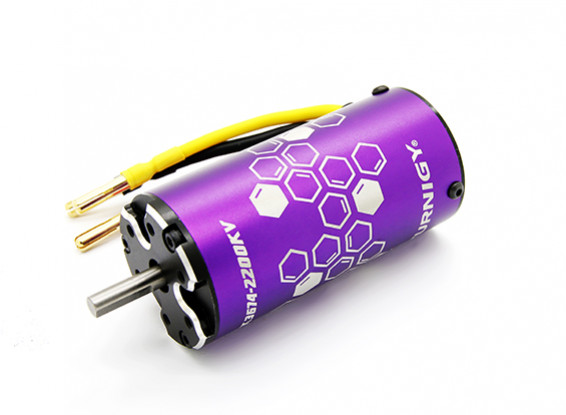
\includegraphics[width=8cm]{imagens/Turnigy XK3674-2200KV.jpg}
    \caption*{Fonte:\cite{turnigyMotor}.}
 \label{Motor Brushless Turnigy XK3674-2200KV}
\end{figure}

\subsection{Fonte de Alimentação Principal (Bateria)}
Em uma aplicação móvel para o ESC devemos fazer uso de baterias como a única fonte de potência para alimentar todo o sistema. Os valores nominais de tensão e corrente do motor a devem ser supridos pela bateria, por volta de $26V$ e $70A$, mas considerando momentos de pico de corrente como por exemplo, uma situação de rotor travado ou de inversão de sentido de rotação é usada uma margem de segurança arbitrária de $30\%$, logo a bateria deve ser capaz de entregar $91A$ de corrente na descarga, um valor considerado alto para baterias.

Atualmente, a tecnologia de bateria com a maior taxa de descarga disponível comercialmente é a bateria de lítio de polímero (LiPo), podendo atingir taxas de descarga muito altas, que podem ultrapassar a $100C$, dependendo da aplicação e do design. 

Baterias LiPo tem três principais características:
\begin{itemize}
\item Configuração das Células (S): A nomenclatura "S" (do inglês \textit{Series}) indica o número de células de polímero de lítio conectadas eletricamente em série no interior do \textit{pack}. Nesta configuração, a tensão de cada célula se soma enquanto a capacidade de corrente se mantém.
    Considerando a tensão nominal de uma célula LiPo como $3,7V$ e a tensão de carga máxima como $4,2V$, a tensão total do \textit{pack} ($V_{\text{pack}}$) é dada por:
    \begin{equation}
        V_{\text{pack}} = N_S \cdot V_{\text{célula}}
    \end{equation}
    Assim, a bateria $6S$ especificada para este projeto possui 6 células, resultando em uma tensão nominal de $22,2V$ e uma tensão máxima de $25,2V$ (plenamente carregada). Este parâmetro é crítico para o dimensionamento do $K_V$ do motor e da tensão máxima dos MOSFETs; 
\item Capacidade: Indica a quantidade de carga que a bateria pode fornecer antes de ser descarregada completamente, Normalmente é medida em miliampere-horas ($mAh$) ou ampere-horas ($Ah$);
\item Taxa de Descarga (ou \textit{C-rate}): Define a quantidade de corrente que a bateria pode fornecer sem danificar-se, é expressa em múltiplos de $C$.
\end{itemize}

Para calcular a corrente que tais baterias conseguem fornecer podemos aplicar a equação \ref{Corrente de uma bateria LiPo}, desconsiderando efeitos dissipativos ou a variação de tensão nominal que varia de acordo com o nível de carga da bateria, vale ressaltar que a capacidade da bateria deve estar em $Ah$.

\begin{equation}
I = C-rate \cdot Capacidade
\label{Corrente de uma bateria LiPo}
\end{equation}


Uma bateria comercial que atende as especificações do projeto é o modelo Turnigy Graphene Panther $1300mAh$ $6S$ $75C$, capaz de fornecer por volta de $97,5A$, superior a margem de segurança estabelecida. Vale ressaltar que a baterias entrega de tensão nominal $22,2V$, inferior a tensão nominal o que para motores BLDC não é um problema, resultando apenas na redução da  sua velocidade nominal de $55440 RPM$ para $48840RPM$ a vazio, uma redução de aproximadamente $12\%$. 

\begin{figure}[h]
    \centering
    \caption{Turnigy Graphene Panther $1300mAh$ $6S$ $75C$.}
    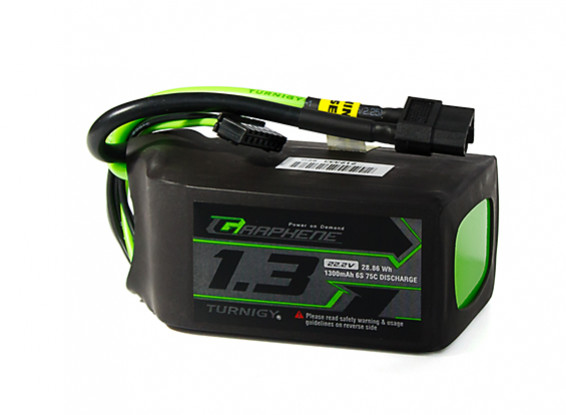
\includegraphics[width=9cm]{imagens/Turnigy Graphene Panther 1300mAh 6S 75C.jpg}
    \caption*{Fonte:\cite{turnigyBattery}.}
 \label{Turnigy Graphene Panther 1300mAh 6S 75C}
\end{figure}

\subsection{Sistema de Proteção Contra Sobrecorrentes}

Dada a baixa resistência interna das baterias de Lítio-Polímero (LiPo) e a alta capacidade de corrente do sistema ($>90 \text{ A}$), um eventual curto-circuito no estágio de potência resultaria em correntes de falha de magnitude catastrófica, com risco real de incêndio e explosão da fonte de energia.

Para mitigar este risco, projetou-se um sistema de proteção passiva composto por um fusível do tipo \textbf{MIDI} de $100 A$, instalado em série com o cabo positivo da bateria, externo à placa de circuito impresso (PCB). Esta topologia foi escolhida baseada em dois critérios:

\begin{itemize}
    \item \textbf{Tipo de Fusível (MIDI):} Diferente dos fusíveis de lâmina automotivos comuns (ATO/ATC), o padrão MIDI possui terminais para fixação por parafusos (M5 ou M6). Isso garante uma pressão de contato elevada, minimizando a resistência de contato ($R_{contato}$) e, consequentemente, o aquecimento indesejado no ponto de conexão sob altas correntes.
    
    \item \textbf{Instalação Externa (Off-Board):} A alocação do fusível no cabo, ao invés da PCB, preserva a integridade das trilhas de cobre em caso de fusão violenta do elemento condutor. Além disso, facilita a manutenção em campo e remove uma fonte de calor concentrada de perto dos transistores de potência.
\end{itemize}

O dimensionamento de $100 A$ oferece uma margem de segurança de aproximadamente $10\%$ sobre a corrente de pico estimada do motor ($90 A$), garantindo que o dispositivo atue apenas em casos de falha real (curto-circuito ou travamento mecânico do rotor), sem interrupções espúrias durante a operação nominal.

\subsection{Filtragem do Barramento DC (Link DC)}

Considerando a bateria LiPo como fonte primária de energia, e sabendo que a indutância dos cabos de alimentação pode gerar transientes destrutivos, projetou-se um estágio de filtragem para o barramento DC.

O dimensionamento dos capacitores do \textit{Link DC} priorizou a minimização da Resistência Série Equivalente (ESR) para evitar o superaquecimento causado pela corrente de ripple. A capacitância mínima ($C_{bus}$) foi estipulada seguindo a regra prática de engenharia para ESCs de alta performance, que recomenda aproximadamente $220\mu F$ para cada $20A$ de corrente de fase:

\begin{equation}
    C_{bus} \approx \frac{I_{peak}}{20} \cdot 220\mu F = \frac{90}{20} \cdot 220\mu F \approx 990 \mu F
\end{equation}

Dessa forma, a topologia final do barramento de entrada é composta por:
\begin{itemize}
    \item Conector de alta corrente XT90 (anti-centelha) para conexão com a bateria;
    \item Dois capacitores eletrolíticos \textit{Low-ESR} de \textbf{$470\mu F$ / $35V$} ligados em paralelo (Total: $940\mu F$), posicionados o mais próximo possível dos drenos dos MOSFETs de alta para minimizar o loop de indutância.
\end{itemize}

Esta escolha assegura que o banco de capacitores suporte a corrente $I_{RMS}$ estimada do inversor, mantendo a temperatura de operação dentro dos limites seguros especificados para a série \textit{Low-ESR}.

\subsection{Dimensionamento do Inversor (MOSFETs)}
Para o estágio de comutação da ponte inversora trifásica, a escolha do MOSFET foi governada por dois parâmetros críticos: a tensão de ruptura dreno-fonte ($V_{DSS}$), representa o limite máximo de tensão que o dispositivo suporta em seus terminais principais enquanto está em estado de não-condução e a capacidade de dissipação térmica. Considerando que a bateria 6S carregada atinge $25,2V$, e prevendo picos de tensão indutiva ($V_{spike}$) durante o chaveamento, selecionou-se o modelo \textbf{IRFS7530TRL7PP}. Este componente possui um $V_{DSS}$ de $60V$, oferecendo uma margem de segurança superior a 100\% em relação à tensão do barramento DC.

A validação térmica foi realizada considerando a resistência em condução ($R_{DS(on)}$) máxima do componente, que é de aproximadamente $1,4 m\Omega$. Para a corrente de pico projetada de $91A$, a potência dissipada estimada ($P_{diss}$) é dada por:

\begin{equation}
    P_{diss} = I^2 \cdot R_{DS(on)} = 91^2 \cdot 0,0014 \approx 11,6 W
\end{equation}

Embora o encapsulamento D2PAK-7 suporte altas correntes, a dissipação de aproximadamente $11,6W$ exige o uso de uma área de cobre estendida na PCB ou acoplamento com dissipador térmico externo para manter a temperatura de junção dentro dos limites operacionais seguros.



\subsection{Driver de Gate e Circuito de Bootstrap}
O microcontroladores no geral operam com lógica de $3,3V$ ou $5V$, tensão insuficiente para saturar o gate dos MOSFETs de potência, que requerem tipicamente entre $10V$ e $15V$ para garantir a mínima resistência $R_{DS(on)}$. Além disso, o acionamento dos MOSFETs do lado alto (\textit{High-Side}) exige uma tensão flutuante superior à tensão da bateria.

Para solucionar essa interface, foi selecionado o driver de meia-ponte \textbf{IR2110}, capaz de fornecer correntes de pico de até $2A$ para carga e descarga rápida da capacitância de gate ($Q_g$). O driver é alimentado com $15V$ (derivados do circuito BEC), garantindo a saturação completa dos transistores.

De acordo com o datasheet do IRFS7530, a resistência interna de gate típica é de $2,1 \Omega$. Para limitar a corrente de source ($I_{source}$) ao máximo de $2A$ sob a tensão de alimentação de $15V$, a resistência total do caminho de gate deve ser:

\begin{equation}
    R_{total} \geq \frac{V_{drv}}{I_{max}} = \frac{15V}{2A} = 7,5 \Omega
\end{equation}

Subtraindo a resistência interna do componente, obtém-se o valor mínimo teórico para o resistor externo:

\begin{equation}
    R_{g,ext} = R_{total} - R_{G,int} = 7,5 \Omega - 2,1 \Omega = 5,4 \Omega
\end{equation}

Para assegurar uma margem de segurança e maior amortecimento, selecionou-se o valor comercial de \textbf{$10 \Omega$}. Com este valor, o tempo de comutação estimado ($t_{sw}$) para a carga total de gate ($Q_g \approx 360nC$) será:

\begin{equation}
    I_{med} \approx \frac{V_{drv}}{R_{g,ext} + R_{G,int}} = \frac{15V}{12,1 \Omega} \approx 1,24 A
\end{equation}

\begin{equation}
    t_{sw} \approx \frac{Q_g}{I_{med}} = \frac{360nC}{1,24A} \approx 290 ns
\end{equation}

Este tempo de transição de aproximadamente $290ns$ é adequado para a frequência de PWM do projeto (tipicamente $20kHz$ a $40kHz$), representando menos de $1,5\%$ do período total, o que garante baixas perdas por comutação sem comprometer a estabilidade eletromagnética.

Para o acionamento do \textit{High-Side}, utiliza-se a técnica de \textit{Bootstrap}. O capacitor de bootstrap ($C_{boot}$) foi dimensionado para sustentar a carga do gate durante o período de condução. Adotou-se o critério de projeto que recomenda que o capacitor seja capaz de armazenar uma carga pelo menos 15 vezes superior à carga total de gate ($Q_g$) do MOSFET \cite{adamsDT98}. Considerando o IRFS7530 com $Q_g \approx 360nC$:

\begin{equation}
    Q_{min} = 15 \cdot Q_g = 15 \cdot 360nC = 5,4 \mu C
\end{equation}

Para o banco de capacitores, optou-se por uma associação em paralelo de um capacitor eletrolítico de $10\mu F$ (reserva de energia) e um cerâmico de $100nF$ (para resposta em alta frequência). Alimentados pela tensão de $15V$ do driver, a carga total armazenada é:

\begin{equation}
    Q_{arm} = C_{boot} \cdot V_{drv} = 10\mu F \cdot 15V = 150 \mu C
\end{equation}

O valor obtido ($150 \mu C$) é significativamente superior ao mínimo requerido ($5,4 \mu C$), garantindo robustez. Além disso, a queda de tensão estimada no capacitor a cada ciclo de comutação ($\Delta V_{boot}$) é desprezível:

\begin{equation}
    \Delta V_{boot} = \frac{Q_g}{C_{boot}} = \frac{360nC}{10\mu F} = 0,036V
\end{equation}

Essa queda de apenas $36mV$ (0,24\% da tensão de alimentação) assegura que a tensão $V_{GS}$ aplicada ao MOSFET permaneça estável, garantindo a saturação completa do semicondutor.

\subsection{Determinação da Frequência de Chaveamento}

A definição da frequência de chaveamento ($f_{sw}$) é um parâmetro crítico no projeto de inversores de frequência de alta corrente, pois representa um \textit{trade-off} direto entre eficiência térmica, qualidade da forma de onda e conforto acústico. Para este projeto, optou-se pela frequência de \textbf{20 kHz}.

Esta escolha fundamenta-se em três critérios de engenharia principais e na validação de compatibilidade dos componentes selecionados:

\subsubsection{Análise de Perdas por Comutação}
As perdas de potência em um MOSFET durante a comutação ($P_{sw}$) são diretamente proporcionais à frequência de operação, conforme estabelecido na Equação \ref{eq:perdas} \cite{rashid2014power}:

\begin{equation} \label{eq:perdas}
P_{sw} = \frac{1}{2} V_{d} \cdot I_{o} \cdot (t_{on} + t_{off}) \cdot f_{sw}
\end{equation}

Onde $V_d$ é a tensão do barramento, $I_o$ a corrente de carga e $t_{on}/t_{off}$ os tempos de comutação.
O projeto utiliza transistores automotivos IRFS7530, que, embora robustos, apresentam uma carga total de gate ($Q_g$) significativa. A elevação da frequência para valores típicos de aeromodelismo (como $48 kHz$ ou $96 kHz$) resultaria em uma dissipação térmica excessiva nos semicondutores, exigindo sistemas de arrefecimento incompatíveis com o volume disponível. A frequência de $20 kHz$ mantém as perdas em um nível gerenciável pela dissipação passiva projetada.

\subsubsection{Mitigação de Ruído Acústico}
A operação de motores elétricos gera ruído audível devido à magnetostrição nas lâminas do estator e nas bobinas, excitadas pelos harmônicos da corrente PWM. Segundo Mohan, Undeland e Robbins (2003), recomenda-se que a frequência de chaveamento seja situada acima do limiar da audição humana.
Ao fixar $f_{sw}$ em $20 kHz$, o sistema opera na região ultrassônica, eliminando o zumbido agudo característico de inversores que operam em faixas inferiores (como $8 kHz$ ou $12 kHz$), garantindo conforto acústico na operação do veículo.

\subsubsection{Ripple de Corrente e Torque}
Para garantir um torque constante, a frequência de chaveamento deve ser suficientemente alta para interagir com a indutância do motor, limitando a ondulação de corrente (\textit{ripple}). Devido à ausência de dados de indutância e resistência no datasheet do fabricante (Turnigy), consideraram-se os valores típicos para motores BLDC de 4 polos (classe 3674) encontrados na literatura \cite{hanselman2003brushless}: indutância de fase na ordem de $L \approx 20 \mu H$ e resistência de $R \approx 10 m\Omega$.

Isso resulta em uma constante de tempo elétrica estimada de $\tau = L/R \approx 2 \text{ ms}$. Dado que o período de chaveamento a 20 kHz é de $T = 50 \mu s$, observa-se que $T \ll \tau$. Essa margem garante que a dinâmica elétrica do motor seja significativamente mais lenta que o chaveamento, assegurando a operação no modo de condução contínua com baixa ondulação de corrente \cite{hanselman2003brushless}.

\subsubsection{Validação da Compatibilidade do Driver}
Foi realizada a validação teórica do driver de gate IR2110 para assegurar sua operação estável na frequência definida. Segundo o datasheet do fabricante \cite{infineon2005}, o componente apresenta tempos de propagação típicos de $t_{on} = 120 \text{ ns}$ e $t_{off} = 94 \text{ ns}$. Considerando o período de $50 \mu s$, os atrasos do driver representam menos de $0,5\%$ do ciclo total, sendo desprezíveis para a dinâmica do controle.

Adicionalmente, calculou-se a corrente média de gate ($I_{g,avg}$) necessária para comutar os MOSFETs, considerando o pior caso de carga de gate ($Q_{g,max} = 354 \text{ nC}$) especificado no datasheet do IRFS7530 \cite{infineon7530}, conforme a Equação \ref{eq:igavg}:

\begin{equation} \label{eq:igavg}
I_{g,avg} = Q_{g,max} \cdot f_{sw} \approx 354 \text{ nC} \cdot 20 \text{ kHz} \approx 7,08 \text{ mA}
\end{equation}

O valor calculado de $7,08 mA$ está amplamente dentro da capacidade de dissipação térmica do IR2110 e situa-se muito abaixo do seu limite de corrente de pico ($2 A$), confirmando que o estágio de acionamento operará em regime seguro.

A frequência de $20 kHz$ foi validada teoricamente como o ponto ótimo de operação, equilibrando a minimização das perdas térmicas com a operação silenciosa e a integridade dos componentes de acionamento.

\subsection{Fonte de Alimentação Auxiliar}
Existem duas abordagens possíveis para a alimentação do microcontrolador e drivers: utilizar uma segunda bateria ou reduzir o nível de tensão da bateria principal. Para otimizar peso e volume, optou-se por um circuito BEC (\textit{Battery Elimination Circuit}).

Dentre as topologias disponíveis, destacam-se os conversores buck (step-down). O conversor Buck é amplamente utilizado para a redução de tensão, operando com elevada eficiência (tipicamente superior a $85\%$) \cite{TIBuckCalculation}. No projeto será aplicado o módulo comercial de baixo custo \textbf{LM2596}, um conversor buck de $150kHz$ e $3A$. O sistema é configurado em cascata: a tensão da bateria ($22,2V - 25,2V$) é regulada para $15V$ para alimentar os drivers IR2110, e subsequentemente reduzida para $5V/3,3V$ para o microcontrolador ESP32.

\begin{figure}[h] 
    \centering 
    \caption{Módulo Comercial LM2596.} 
    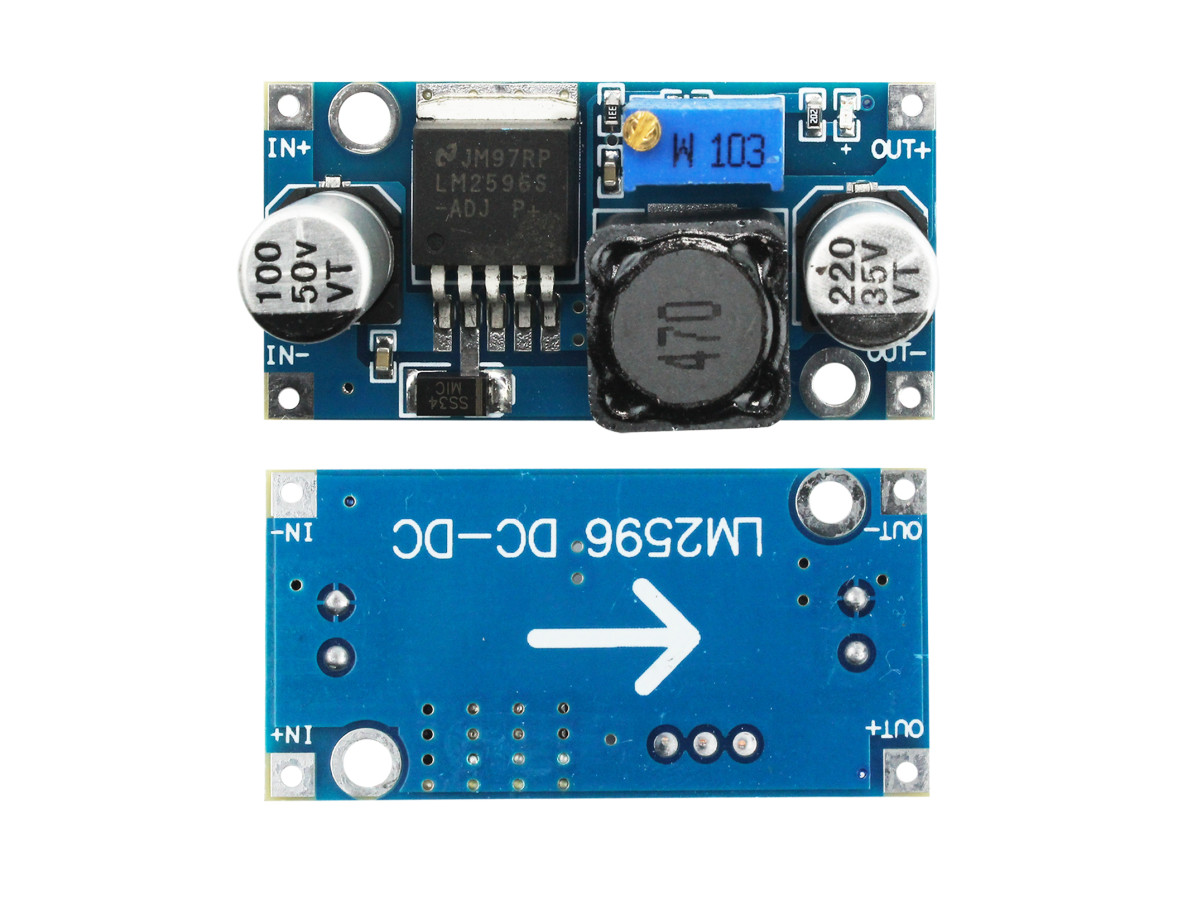
\includegraphics[width=7cm]{imagens/Módulo LM2596.jpg} 
    \caption*{Fonte:\cite{usinaInfoLM2596}.}
\end{figure}

\subsection{Sensoriamento de Corrente e Proteção (Shunt)}

Para implementar a proteção contra sobrecorrente e monitorar o consumo do sistema em tempo real, adotou-se a topologia de sensoriamento resistivo no lado baixo (\textit{Low-Side Current Sensing}). A escolha por um resistor \textit{shunt} em detrimento de sensores baseados em Efeito Hall (como a família ACS7xx) justifica-se pela necessidade de resposta em frequência instantânea para a proteção de curto-circuito, eliminando os atrasos de propagação e as não-linearidades típicas de sensores magnéticos integrados.

O dimensionamento do resistor $R_{shunt}$ buscou minimizar as perdas por condução sem comprometer a relação sinal-ruído. Selecionou-se um resistor de liga metálica de \textbf{$0,5 m\Omega$}. Considerando a corrente de pico de projeto ($I_{peak} \approx 91A$), a potência dissipada por efeito Joule no elemento sensor é:

\begin{equation}
    P_{shunt} = I_{peak}^2 \cdot R_{shunt} = 91^2 \cdot 0,0005 \approx 4,14 W
\end{equation}

Embora a dissipação de aproximadamente $4W$ exija um componente com encapsulamento de potência (formato 3920 ou 5930), a análise de impacto na eficiência global do sistema demonstra a viabilidade da solução. Comparando a perda no sensor com a potência elétrica total entregue ao motor na tensão nominal ($22,2V$):

\begin{equation}
    P_{sys} \approx V_{bat} \cdot I_{peak} = 22,2V \cdot 91A \approx 2020 W
\end{equation}

\begin{equation}
    \eta_{loss} = \frac{P_{shunt}}{P_{sys}} = \frac{4,14W}{2020W} \approx 0,2\%
\end{equation}

A perda de apenas $0,2\%$ é considerada desprezível frente às perdas de comutação e condução dos MOSFETs, validando a aplicação.

Para o condicionamento do sinal, a queda de tensão máxima gerada nos terminais do \textit{shunt} será de $V_{sense} = 91A \cdot 0,5m\Omega = 45,5mV$. Como essa amplitude é insuficiente para a faixa dinâmica do ADC do ESP32 ($0-3,3V$), projetou-se um estágio amplificador não-inversor. O ganho ($A_v$) necessário para mapear a corrente de pico na escala completa é:

\begin{equation}
    A_v = \frac{V_{ADC(max)}}{V_{sense}} = \frac{3,3V}{0,0455V} \approx 72,5
\end{equation}

Fixou-se o ganho em $A_v = 73$, utilizando resistores de precisão de 1\% na malha de realimentação do Amplificador Operacional, garantindo que a proteção atue precisamente antes dos limites térmicos do inversor serem atingidos.

\section{Sistema de Controle e Firmware}
O controle lógico do inversor é centralizado no microcontrolador, responsável pela leitura de sinais, implementação da máquina de estados de comutação e geração dos sinais PWM.

\subsection{O Microcontrolador ESP32}
Para essa aplicação, foi selecionado o ESP32-DevKit C. Utilizando como principal elemento o módulo ESP32-WROOM-32, ele apresenta uma solução robusta para controle em tempo real. Capaz de operar em velocidades de clock de até $240 MHz$, permite a execução paralela de tarefas, característica crítica para sistemas ESC. A resolução de 16 bits dos geradores PWM amplia a precisão no controle da velocidade.

\begin{figure}[H]
    \centering
    \caption{Visão Geral do Microcontrolador ESP32-DevKit C.}
    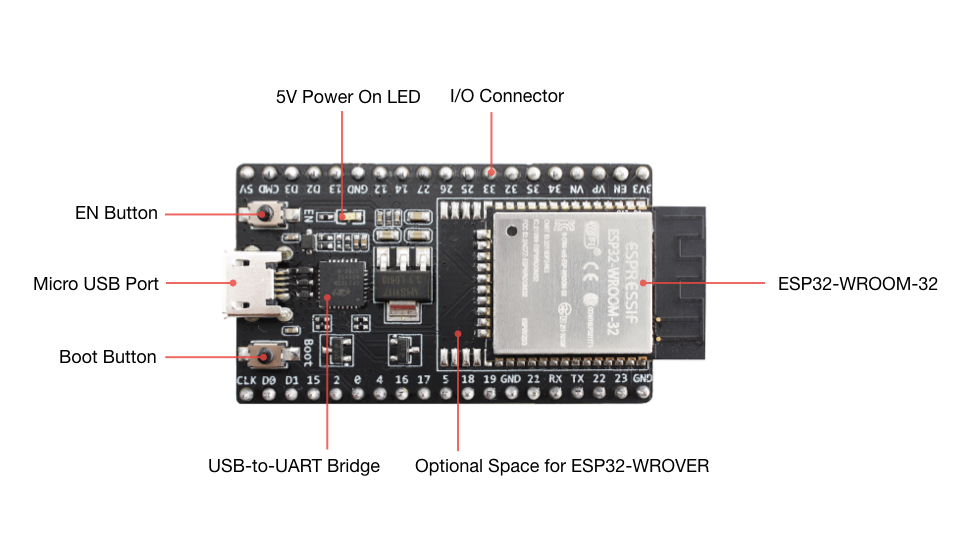
\includegraphics[width=10cm]{imagens/esp32-devkitc-v4-functional-overview.jpg}
    \caption*{Fonte:\cite{ESP32-DevKitCOverview}.}
 \label{esp32DevkitC}
\end{figure}

\begin{figure}[H]
    \centering
    \caption{Pinagem do Microcontrolador ESP32-DevKit C.}
    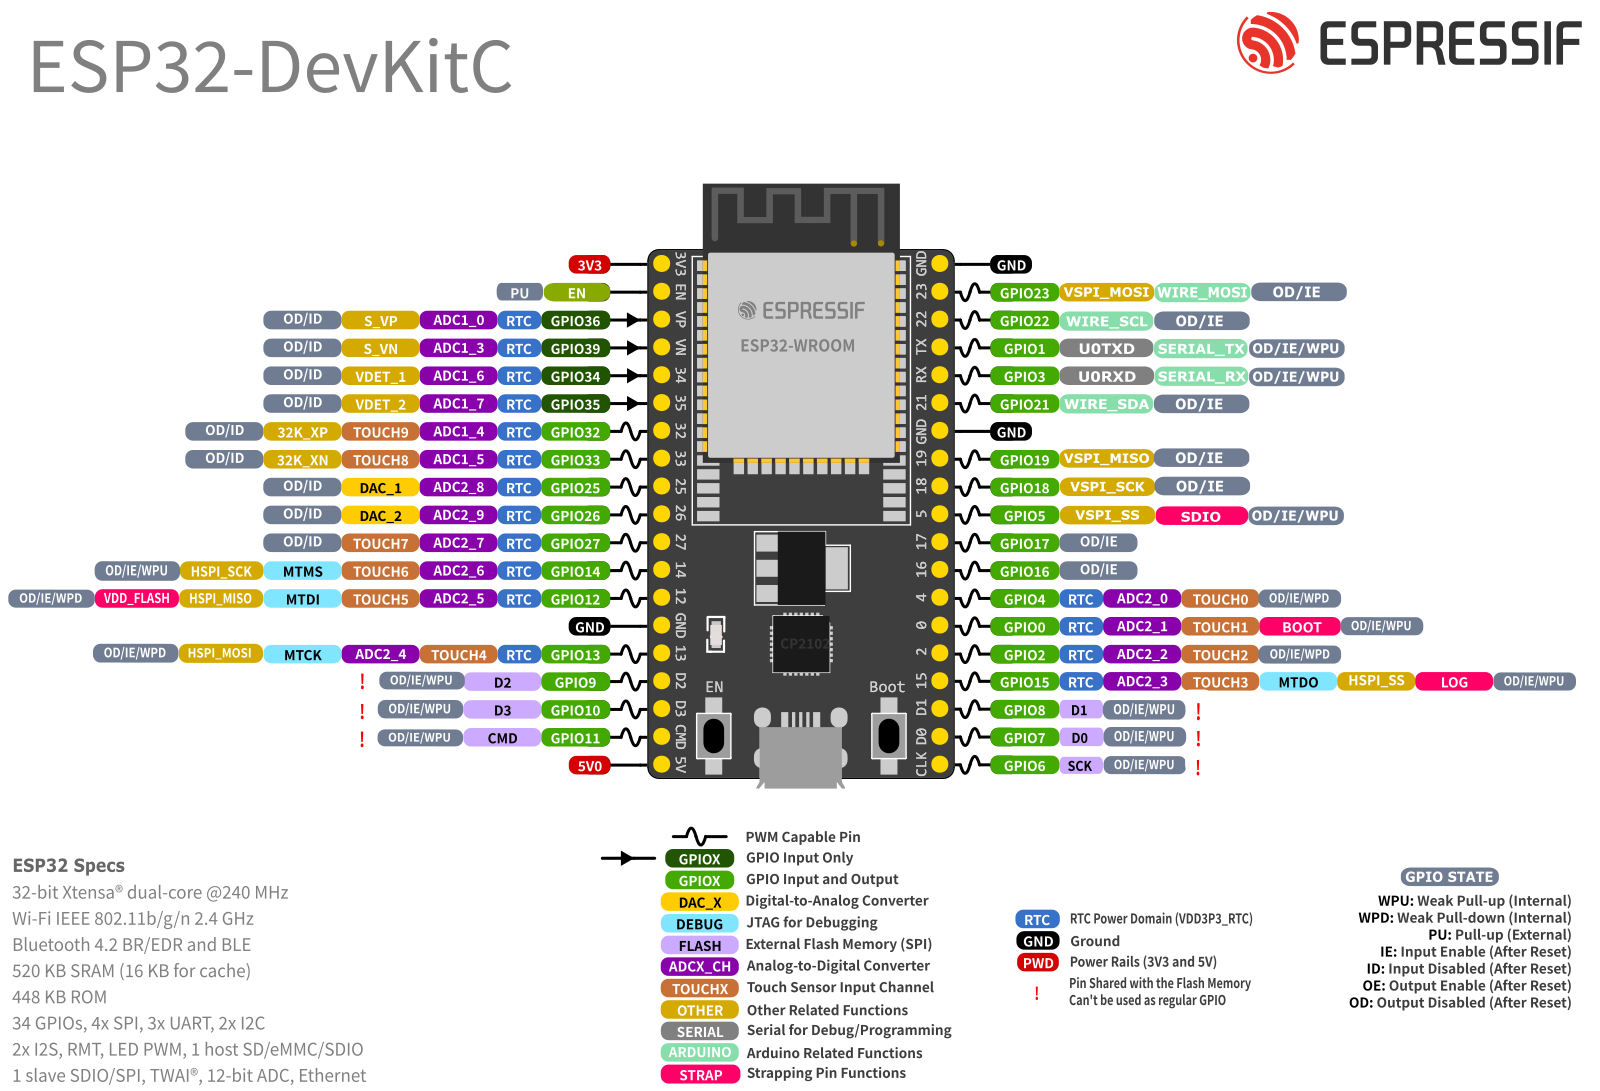
\includegraphics[width=16cm]{imagens/esp32_devkitC_v4_pinlayout.png}
    \caption*{Fonte:\cite{ESP32-DevKitCOverview}.}
 \label{esp32DevkitCPinLayout}
\end{figure}

Apesar dessas vantagens, os níveis lógicos de $3,3V$ exigiram o uso dos drivers IR2110 mencionados anteriormente para a interface com a potência.

\subsection{Lógica de Comutação de Seis Passos}
A lógica de chaveamento constitui o núcleo funcional do ESC. Nesta abordagem, utiliza-se a comutação de seis passos em malha aberta (\textit{Sensorless}). A ponte inversora trifásica é acionada de forma que apenas dois MOSFETs conduzam simultaneamente a cada passo, criando um campo magnético giratório que avança em incrementos de $60^{\circ}$.

\begin{table}[H]
    \centering
    \caption{Sequência de Comutação de Seis Passos e Estado dos MOSFETs}
    \label{tab:logica_seis_passos}
    \begin{tabular}{@{}cccccccc@{}} 
        \toprule
        \textbf{Passo} & \textbf{Pos. Elétrica} & \textbf{High A} & \textbf{Low B} & \textbf{High C} & \textbf{Low A} & \textbf{High B} & \textbf{Low C} \\ \midrule
        1 & 0° -- 60°   & ON & ON  & OFF & OFF & OFF & OFF \\
        2 & 60° -- 120°  & ON & OFF & OFF & OFF & OFF & ON  \\
        3 & 120° -- 180° & OFF& OFF & ON  & OFF & ON  & OFF \\
        4 & 180° -- 240° & OFF& OFF & ON  & ON  & OFF & OFF \\
        5 & 240° -- 300° & OFF& ON  & OFF & ON  & OFF & OFF \\
        6 & 300° -- 360° & OFF& OFF & OFF & OFF & ON  & ON  \\ \bottomrule
    \end{tabular}
    \caption*{Fonte: Elaborado pelo autor.}
\end{table}

\subsection{Implementação Prática com o Periférico MCPWM}
A implementação da comutação no firmware utiliza o periférico dedicado \textit{Motor Control Pulse Width Modulator} (MCPWM) do ESP32 \cite{esp32-technical-reference-manual}. Este módulo desonera a CPU da geração de sinais e insere automaticamente o tempo morto (\textit{Dead Time}) necessário para evitar curto-circuitos na ponte H (shoot-through).

A configuração segue o mapeamento da Tabela \ref{tab:mcpwm_map}, onde o \textit{Duty Cycle} é aplicado ao transistor do lado alto (High-Side) para controle de corrente, enquanto o lado baixo (Low-Side) é mantido em condução plena ou chaveado de forma complementar, dependendo da estratégia de frenagem regenerativa desejada.

\begin{table}[H]
    \centering
    \caption{Mapeamento dos Estados de Comutação para os Geradores MCPWM do ESP32}
    \label{tab:mcpwm_map}
    \resizebox{\textwidth}{!}{%
        \begin{tabular}{@{}ccccccc@{}}
            \toprule
            \textbf{Passo} & \textbf{Fases Energizadas} & \textbf{High-Side} & \textbf{Low-Side} & \textbf{OPR 0 (A)} & \textbf{OPR 1 (B)} & \textbf{OPR 2 (C)} \\ \midrule
            1 & A+ B- & T1 & T4 & PWM / LOW & LOW / ACTIVE & Hi-Z / Hi-Z \\
            2 & A+ C- & T1 & T6 & PWM / LOW & Hi-Z / Hi-Z & LOW / ACTIVE \\
            3 & B+ C- & T3 & T6 & Hi-Z / Hi-Z & PWM / LOW & LOW / ACTIVE \\
            4 & B+ A- & T3 & T2 & LOW / ACTIVE & PWM / LOW & Hi-Z / Hi-Z \\
            5 & C+ A- & T5 & T2 & LOW / ACTIVE & Hi-Z / Hi-Z & PWM / LOW \\
            6 & C+ B- & T5 & T4 & Hi-Z / Hi-Z & LOW / ACTIVE & PWM / LOW \\ \bottomrule
        \end{tabular}
    }
    \flushleft
    \footnotesize{\textit{Nota:} "PWM / LOW" indica modulação. "LOW / ACTIVE" indica condução ao terra. "Hi-Z" alta impedância.} 
\end{table}

\subsection{Estratégia de Partida e Transição para Malha Fechada}

A técnica de detecção de cruzamento por zero da FCEM possui uma limitação física intrínseca: a amplitude da FCEM é proporcional à velocidade do rotor ($e = K_e \cdot \omega$). Na partida ($t=0$), a FCEM é nula, impossibilitando a determinação da posição do rotor pelos comparadores. Para contornar isso, implementou-se uma máquina de estados finitos composta por três estágios:

\begin{enumerate}
    \item \textbf{Alinhamento (Estágio Estático):} 
    Aplica-se uma tensão constante em um par de fases específico (ex: Fase A em High, Fase B em Low) por um período fixo de $500ms$. Isso força o rotor a se alinhar fisicamente com o campo magnético do estator, estabelecendo uma posição inicial conhecida ($\theta_0$) antes do início do movimento.
    
    \item \textbf{Aceleração em Malha Aberta (Blind Commutation):} 
    A partir da posição conhecida, o controlador inicia a sequência de comutação de seis passos utilizando um temporizador interno, ignorando os sinais dos comparadores. A frequência de comutação é incrementada linearmente (Rampa) para acelerar o motor.
    
    Este estágio é mantido pelo menor tempo possível, apenas o suficiente para que o motor atinja cerca de 5\% a 10\% da sua velocidade nominal, ponto em que a amplitude da FCEM supera o limiar de histerese e ruído dos comparadores LM339.
    
    \item \textbf{Transição e Auto-Comutação (Closed-Loop):} 
    Assim que o microcontrolador detecta uma sequência válida de cruzamentos por zero (ZCD) nos comparadores, o sistema realiza o \textit{handover}. O temporizador de malha aberta é desativado e o controle passa a ser orientado a eventos: cada detecção de ZCD dispara uma interrupção que, após um atraso calculado de $30^\circ$ elétricos, executa a próxima comutação de fase. A partir deste momento, o motor opera em malha fechada, auto-sincronizado.
\end{enumerate}

Essa abordagem híbrida elimina a necessidade de rampas longas e ineficientes, garantindo uma partida robusta e uma operação contínua otimizada.


\section{Sistema de Realimentação e Detecção de Cruzamento por Zero}

Para viabilizar a operação em malha fechada sem o uso de sensores de posição dedicados (sensores Hall), implementou-se a técnica de detecção de cruzamento por zero (\textit{Zero-Crossing Detection} - ZCD) da força contraeletromotriz (FCEM). Esta técnica baseia-se no monitoramento da tensão na fase não energizada do motor durante a sequência de comutação de seis passos. O instante em que a FCEM cruza o nível de tensão do ponto neutro do motor indica uma posição angular conhecida do rotor, permitindo a sincronização precisa da comutação eletrônica.

Como o motor utilizado (Turnigy XK3674) possui fechamento interno em triângulo ou estrela sem acesso ao ponto neutro, o sistema de realimentação foi projetado em três estágios: reconstrução do neutro virtual, condicionamento de sinal e comparação.

\subsection{Reconstrução do Neutro Virtual e Divisores de Tensão}

A ausência de um terminal de neutro físico acessível exigiu a criação de um ponto de neutro virtual. Para isso, conectou-se um resistor de $33k\Omega$ em cada uma das três fases do motor ($A, B, C$), unindo as extremidades opostas em um nó comum. Este nó fornece a referência de tensão média do sistema ($V_{ref}$) para os comparadores, conforme topologia clássica para controle trapezoidal \textit{sensorless} \cite{ti2013sensorless}.

Considerando a escalabilidade do projeto para operar com baterias de até 6 células (6S, $\approx 25,2V$), a rede de divisores resistivos foi dimensionada para garantir a segurança do microcontrolador no pior caso de tensão. Utilizou-se uma topologia composta por um resistor de lado alto ($R_{high}$) de $33k\Omega$ e um resistor de lado baixo ($R_{low}$) de $3,3k\Omega$, resultando em um fator de atenuação $\alpha$:

\begin{equation}
    V_{out} = V_{in} \cdot \frac{R_{low}}{R_{high} + R_{low}} = 25,2 \cdot \frac{3,3k}{33k + 3,3k} \approx 2,29V
\end{equation}

Esta configuração garante que a tensão máxima no pino do microcontrolador permaneça abaixo de $3,3V$, preservando uma margem de segurança para picos indutivos (spikes) típicos de comutação.

\subsection{Filtragem de Ruído PWM}

O sinal de tensão proveniente das fases contém componentes de alta frequência resultantes da modulação por largura de pulso (PWM), tipicamente na ordem de $20kHz$. Para evitar múltiplos disparos falsos no comparador, adicionou-se um capacitor cerâmico ($C_f$) de $10nF$ em paralelo com o resistor $R_{low}$, formando um filtro passa-baixa passivo de primeira ordem. A frequência de corte ($f_c$) foi dimensionada para preservar a componente fundamental da FCEM (proporcional à velocidade do motor) enquanto atenua o ruído de chaveamento:

\begin{equation}
    f_c = \frac{1}{2\pi \cdot (R_{high} || R_{low}) \cdot C_f} \approx \frac{1}{2\pi \cdot 3000 \cdot 10 \cdot 10^{-9}} \approx 5,3kHz
\end{equation}

\subsection{Análise e Compensação do Atraso de Fase do Filtro}

A introdução do capacitor $C_f$ no circuito divisor de tensão, embora essencial para a integridade do sinal, insere um polo no sistema que causa um atraso de fase ($\phi$) dependente da frequência. Em um filtro RC de primeira ordem, o atraso de fase entre o sinal de entrada (BEMF real) e o sinal de saída (lido pelo comparador) é dado por \cite{ti2013sensorless}:

\begin{equation}
    \phi = \arctan(2\pi f_{el} R_{eq} C_f) = \arctan\left(\frac{f_{el}}{f_c}\right)
    \label{eq:phase_lag}
\end{equation}

\noindent onde $f_{el}$ é a frequência elétrica fundamental do motor e $f_c$ é a frequência de corte do filtro ($\approx 5,3kHz$).

Este atraso angular é crítico para o sincronismo da comutação. Na estratégia \textit{sensorless} ideal, a comutação das fases deve ocorrer $30^{\circ}$ elétricos após o cruzamento por zero da BEMF. No entanto, devido ao filtro, o comparador detecta o evento de cruzamento com um atraso de $\phi$ graus. Se o microcontrolador aguardar os $30^{\circ}$ teóricos após essa detecção tardia, a comutação efetiva ocorrerá em $30^{\circ} + \phi$, resultando em uma aplicação de torque fora do ponto de máxima eficiência.

Considerando as especificações do motor Turnigy XK3674 ($2200KV$, 4 polos) operando à tensão nominal de $22,2V$, a velocidade máxima teórica aproxima-se de $48.840$ RPM. A frequência elétrica máxima correspondente é:

\begin{equation}
    f_{el\_max} = \frac{RPM \cdot P}{120} = \frac{48840 \cdot 4}{120} \approx 1.628 \text{ Hz}
\end{equation}

Substituindo na Equação \ref{eq:phase_lag}:

\begin{equation}
    \phi_{max} = \arctan\left(\frac{1628}{5300}\right) \approx 17,07^{\circ}
\end{equation}

Como o atraso máximo projetado ($17,07^{\circ}$) é inferior ao intervalo de comutação padrão ($30^{\circ}$), é possível realizar a compensação via software. A estratégia adotada, alinhada às recomendações da literatura especializada \cite{ti2013sensorless}, consiste em calcular dinamicamente o ângulo de atraso $\phi$ a cada ciclo e ajustar o temporizador de espera ($T_{wait}$):

\begin{equation}
    T_{wait} = T_{30^{\circ}} - T_{lag}
\end{equation}

\noindent Onde $T_{30^{\circ}}$ é o período correspondente a $30^{\circ}$ na velocidade atual e $T_{lag}$ é o tempo equivalente ao atraso de fase do filtro. Essa correção assegura que, mesmo em altas rotações, o alinhamento entre os campos do estator e rotor permaneça ortogonal.

\subsection{Estágio Comparador com LM339}

A digitalização dos sinais analógicos é realizada pelo circuito integrado \textbf{LM339N} (encapsulamento DIP-14), que contém quatro comparadores de tensão independentes. A escolha deste componente justifica-se por sua saída em coletor aberto (\textit{Open-Collector}) \cite{tiLM339}. Esta característica permite que o comparador seja alimentado com uma tensão superior (ex: $5V$ ou $12V$) para garantir a linearidade, enquanto a saída é referenciada ao nível lógico do microcontrolador ($3,3V$) através de resistores de \textit{pull-up} de $10k\Omega$.

O circuito utiliza três comparadores configurados da seguinte forma:
\begin{itemize}
    \item \textbf{Entrada Não-Inversora (+):} Tensão da Fase ($A, B$ ou $C$) atenuada e filtrada.
    \item \textbf{Entrada Inversora (-):} Tensão do Neutro Virtual atenuada.
    \item \textbf{Saída:} Conectada a pinos GPIO do ESP32 configurados para interrupção externa.
\end{itemize}

\subsection{Considerações de Sensibilidade e Escalabilidade}

O dimensionamento dos divisores de tensão impõe um compromisso de engenharia (\textit{trade-off}) entre a proteção contra sobretensão e a sensibilidade em baixas velocidades. Com a atenuação de aproximadamente 11:1, sistemas operando com tensões de barramento menores (ex: baterias 2S ou 3S) ou motores em baixa rotação apresentarão sinais de amplitude reduzida na entrada do comparador.

Para mitigar o risco de instabilidade com sinais pequenos, recomenda-se a implementação de \textbf{histerese} no circuito comparador. Isso pode ser realizado através da realimentação positiva, conectando um resistor de alta impedância (ex: $1M\Omega$) entre a saída do comparador e sua entrada não-inversora.

Ressalta-se que a escalabilidade é limitada por dois fatores físicos:
\begin{enumerate}
    \item \textbf{Limite Inferior (3S):} A tensão mínima de operação é definida pelos drivers de gate (IR2110) e pela tensão de limiar ($V_{GS}$) dos MOSFETs. Operar abaixo de $11,1V$ (3S) sem conversores Boost adicionais coloca os transistores na região linear, causando superaquecimento.
    \item \textbf{Limite Superior (6S):} A tensão máxima é estritamente limitada pela tensão de ruptura ($V_{DSS}$) dos MOSFETs utilizados (IRFS7530, $60V$). Embora baterias 7S ($29,4V$) ou 8S ($33,6V$) pareçam estar dentro do limite estático, os picos indutivos gerados durante a comutação podem atingir o dobro da tensão de barramento, excedendo o $V_{DSS}$ e causando falha catastrófica. Portanto, o limite de 6S ($25,2V$) garante a margem de segurança necessária para a robustez do inversor.
\end{enumerate}

\section{Simulação Computacional}
Para validar a lógica de controle e a integridade dos sinais de disparo antes da montagem física, utiliza-se a simulação computacional. Devido à complexidade dos modelos SPICE proprietários para os drivers de gate, opta-se pelo uso de modelos comportamentais equivalentes em software de simulação de circuitos (ex: LTSpice ou Proteus). A simulação foca na verificação das formas de onda de tensão de linha e de fase, bem como na garantia de que a sequência de seis passos não gera sobreposição de condução nos braços do inversor.

\section{Montagem e Prototipagem}
A etapa final consiste na integração física dos subsistemas. O controlador é montado em uma placa de circuito impresso (PCB) desenhada para suportar as altas correntes do barramento DC, com trilhas reforçadas e planos de terra adequados. O microcontrolador é programado com a lógica desenvolvida e o sistema é submetido a testes de bancada, iniciando com cargas leves e alimentação limitada para verificação de segurança (teste de fumaça), progredindo para o acionamento do motor em rampa de velocidade para validação do protótipo funcional.

Todas as etapas de validação e os resultados obtidos, tanto na simulação quanto nos ensaios práticos, são documentados no capítulo subsequente de Resultados.


\chapter{Resultados e Discussão}
%TODO: Inserir Introdução ao capítulo.

\section{Validação Computacional (Simulação)}
%TODO? Falar sobre a modelagem dos capacitores da simulação?

Para a validação conceitual do hardware de potência antes da montagem física, utilizou-se o software \textbf{LTSpice}. A simulação concentrou-se no estágio de potência do inversor, modelando as chaves semicondutoras e a carga indutiva. Foram elaborados dois cenários de simulação: uma topologia monofásica (meia-ponte) para análise isolada e uma topologia trifásica completa para validação do fluxo de corrente inter-fases (Figura \ref{fig:simulacao_trifasica}).

\begin{figure}[H]
    \centering
    \caption{Esquemático da simulação trifásica do ESC em estado estático de comutação.}
    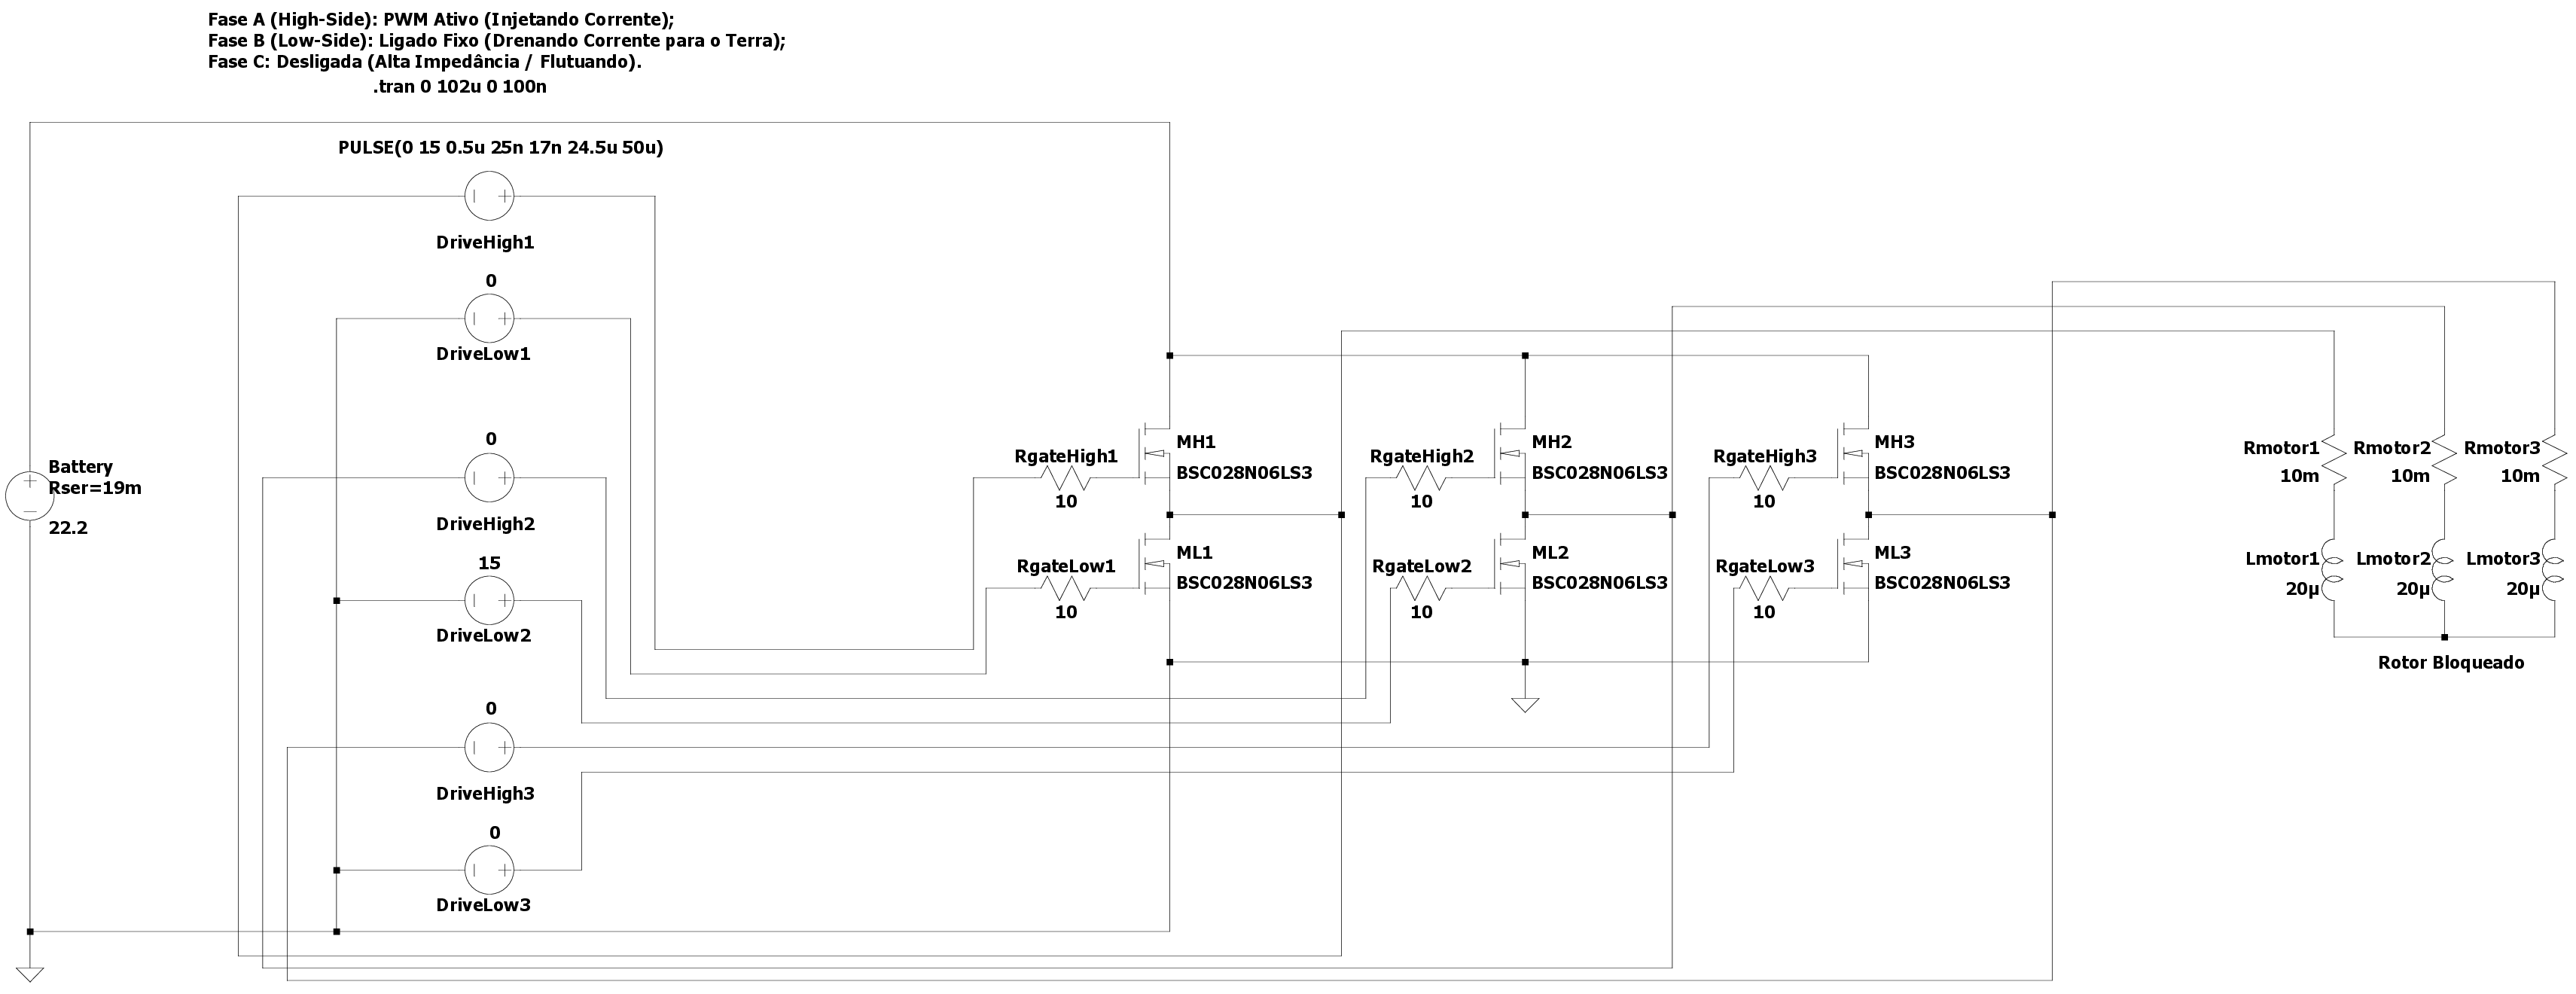
\includegraphics[width=17cm]{Simulation/trifasico.png}
    \caption*{Fonte: Elaborado pelo autor.}
    \label{fig:simulacao_trifasica}
\end{figure}

O circuito é dividido em três blocos funcionais: alimentação, comutação e carga. A fonte de energia primária é modelada por uma fonte DC de $22,2 \: V$ com uma resistência série ($R_{ser}$) de $19 \: m\Omega$, emulando com precisão a dinâmica de descarga e as perdas ôhmicas internas da bateria LiPo 6S definida para o projeto. O estágio de comutação é composto por uma ponte inversora trifásica utilizando transistores MOSFET (modelo comportamental BSC028N06LS3). As portas (\textit{gates}) destes semicondutores são excitadas através de resistores de $10 \: \Omega$, valor projetado para limitar a corrente de pico do \textit{driver} e amortecer ressonâncias (\textit{ringing}) parasitas sem degradar o tempo de comutação. O acionamento através dos \textbf{drivers de gate} foram modeladas utilizando fontes de tensão do tipo pulso. O sinal de acionamento do lado alto (\textit{High-Side}) da Fase A foi definido com os parâmetros \texttt{PULSE(0 15 0 100n 100n 25u 50u)}, forçando a condução do Passo 1 da sequência trapezoidal. Este perfil injeta um sinal com amplitude de $15\text{V}$, estabelecendo uma frequência de chaveamento de \textbf{$20\text{ kHz}$} (período de $50 \mu\text{s}$) e um ciclo de trabalho (\textit{Duty Cycle}) de \textbf{$50\%$}. Os tempos de transição de subida e descida foram definidos em $100\text{ ns}$ para simular o tempo de resposta do gate do \textbf{MOSFET}.

Por fim, o motor BLDC é representado por seu modelo elétrico equivalente de estator, consistindo em três ramos conectados em estrela (neutro comum). Cada fase possui uma resistência de armadura corrigida de $10 \: m\Omega$ em série com uma indutância de $20 \: \mu H$. Esta modelagem a rotor bloqueado força o sistema a operar sob a condição mais severa de estresse elétrico, permitindo avaliar a capacidade máxima de condução de corrente dos transistores e a resposta transitória da rede indutiva sem a oposição da Força Contraeletromotriz (FCEM), garantindo que os resultados da simulação representem o limite operacional do \textit{hardware}. 

Como o esquemático foca na validação da transferência de energia em um instante específico da \textbf{comutação de seis passos} (Fase A injetando corrente e Fase B drenando para o terra), o transistor do lado baixo da Fase A foi mantido em \textbf{corte} ($0\text{V}$ constante). Devido a esta modelagem estática de um único passo, a inserção de um \textbf{tempo morto ($t_{dead}$)} dinâmico não se fez necessária no gerador de pulsos, assumindo-se o isolamento ideal entre os estados de condução. O motor foi adequadamente modelado na condição de \textbf{rotor bloqueado}, respeitando os parâmetros intrínsecos de resistência ($R = 10m \Omega$) e indutância ($L = 20 \mu\text{H}$) por fase.

A Figura \ref{fig:sim_correntes_motor} apresenta os resultados transitórios das correntes de fase ($I_A$, $I_B$ e $I_C$) durante os dois primeiros ciclos de chaveamento do inversor, totalizando $100 \: \mu s$. Observa-se que, durante o primeiro tempo de condução ($T_{on}$) do sinal PWM entre $0$ e $25 \: \mu s$, a corrente $I_A$ ascende de forma linear até atingir o patamar de aproximadamente $13,5 \: A$. Simultaneamente, a corrente $I_B$ apresenta a mesma magnitude, porém com polaridade invertida ($-13,5 \: A$), enquanto a corrente $I_C$ permanece nula, oscilando apenas com os ruídos numéricos do simulador próximos a zero. Durante o tempo de bloqueio do PWM ($T_{off}$) entre $25 \: \mu s$ e $50 \: \mu s$, as correntes $I_A$ e $I_B$ não caem abruptamente para zero, mas sim sofrem um decaimento suave. O ciclo se repete aos $50 \: \mu s$, elevando as correntes ao patamar de $26 \: A$.

\begin{figure}[H]
    \centering
    \caption{Dinâmica das correntes de fase do motor durante os primeiros $100 \: \mu s$ de simulação (Passo 1).}
    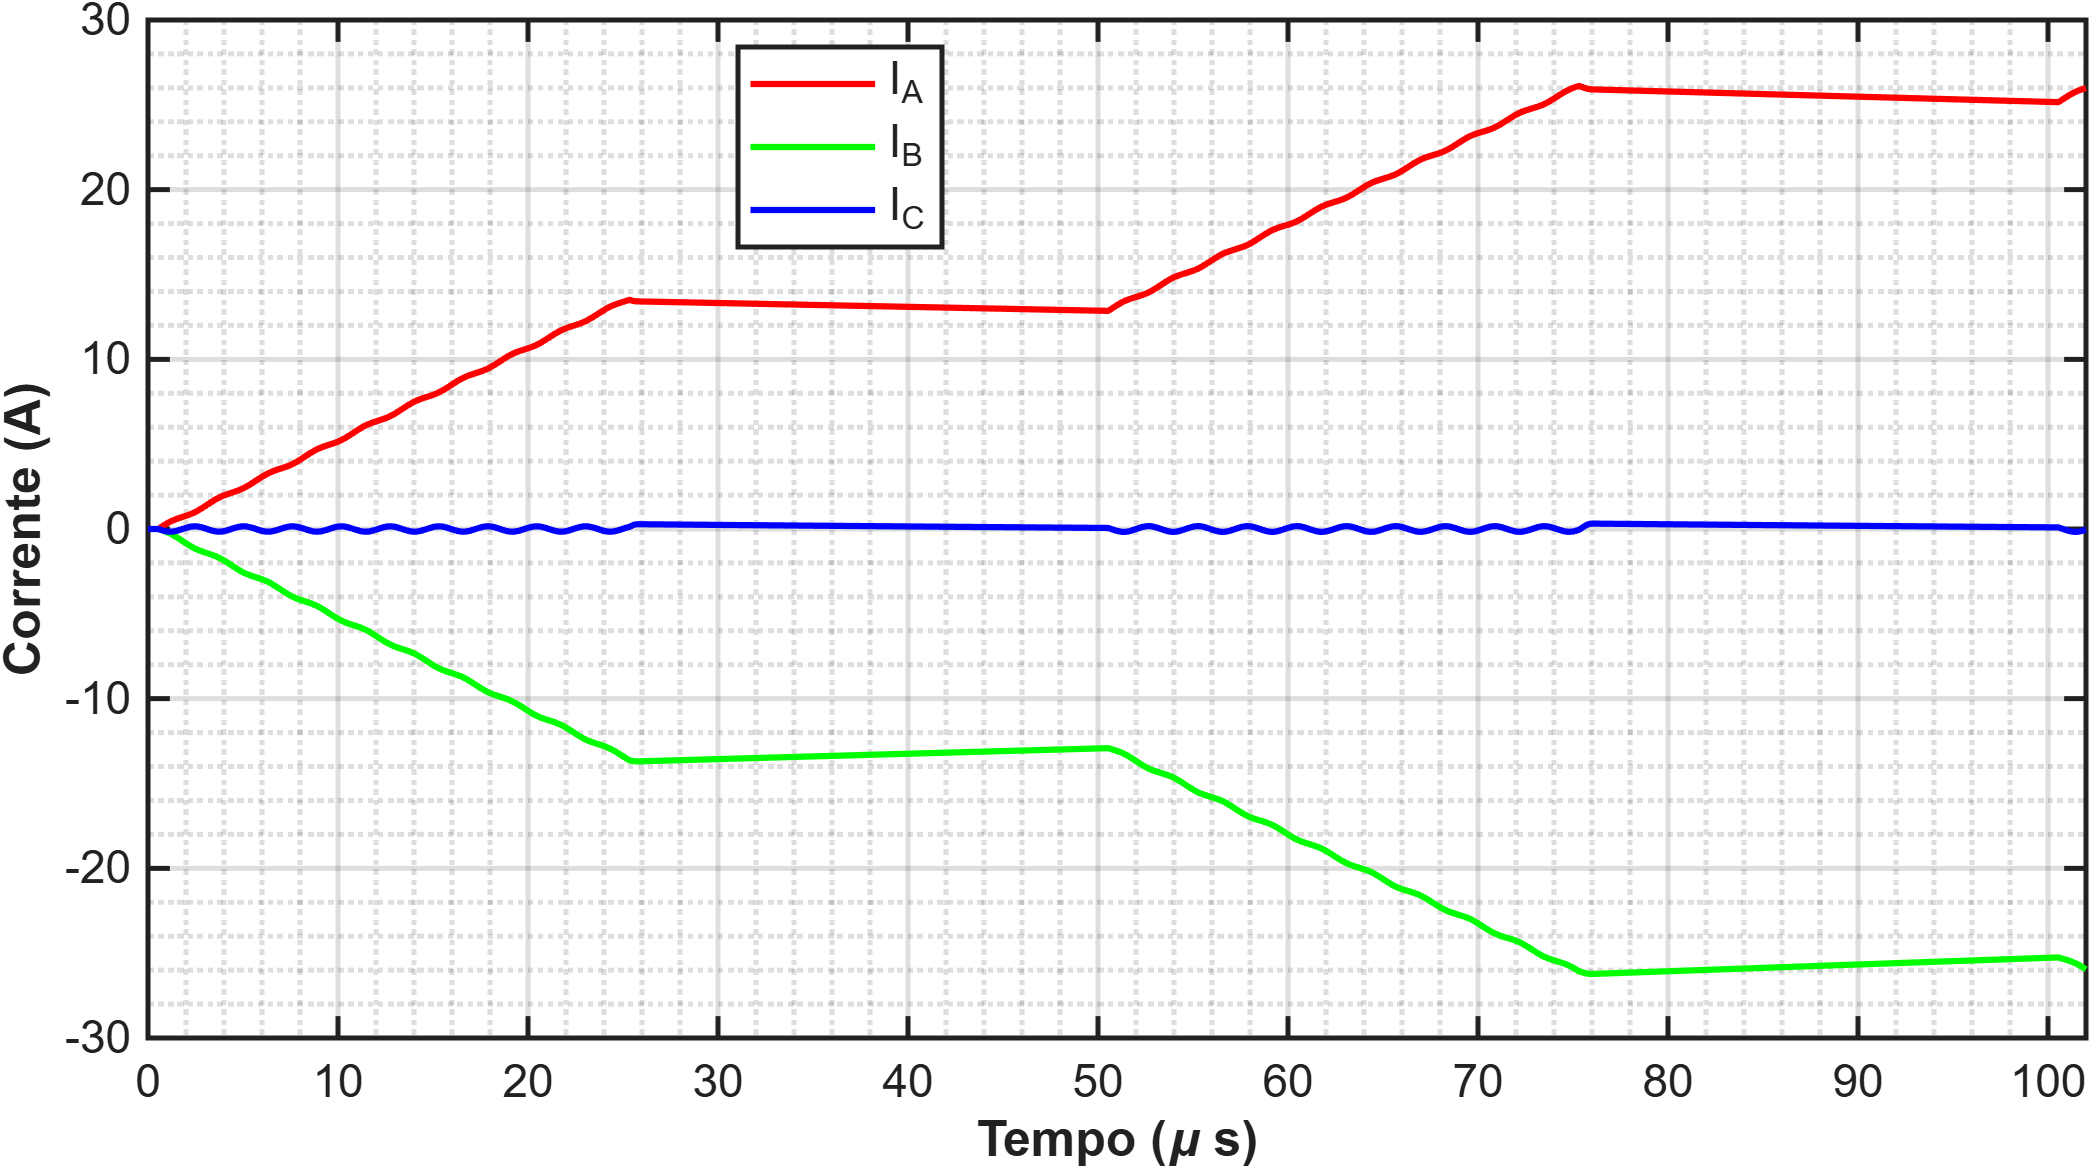
\includegraphics[width=0.8\textwidth]{Simulation/plot_simulacao/1_correntes_motor.png}
    \caption*{Fonte: Elaborado pelo autor.}
    \label{fig:sim_correntes_motor}
\end{figure}

Este comportamento é a resposta direta da excitação do circuito indutivo do estator sob a topologia de modulação \textit{High-Side PWM / Low-Side ON}. Ao disparar o transistor superior da fase A e manter o transistor inferior da fase B em condução plena, estabelece-se um fluxo de elétrons que obrigatoriamente passa por duas bobinas em série ($V = L_{eq} \frac{di}{dt} + R_{eq}i$). A inclinação constante ($di/dt$) da rampa de corrente é ditada pela reatância indutiva nominal do motor. Durante o ciclo $T_{off}$ da chave superior, a energia magnética armazenada na indutância do estator força a manutenção do fluxo de corrente, que encontra caminho através do diodo de roda livre (\textit{freewheeling diodo}) intrínseco ao MOSFET inferior da fase A, justificando a lenta taxa de decaimento observada.

Ao compararmos com o arcabouço teórico, o resultado valida a comutação de seis passos apresentada na Tabela \ref{tab:mcpwm_map}. A frequência estabelecida pelo projeto de $20 \: kHz$ é ratificada pelo período exato de $50 \: \mu s$ entre os picos de chaveamento. Mais importante ainda, a completa inércia da fase C ($I_C \approx 0 \: A$) confirma a eficácia do estado de alta impedância (Hi-Z) no braço inversor não excitado, condição \textit{sine qua non} para a medição livre de distorções da Força Contraeletromotriz (FCEM) na posterior transição para a malha fechada.

A Figura \ref{fig:sim_tensoes_neutro} ilustra o comportamento dinâmico das tensões de fase referenciadas ao ponto neutro da carga ($V_{AN}$, $V_{BN}$ e $V_{CN}$). Durante o período de condução do PWM ($T_{on}$), nota-se que o eixo de oscilação das tensões se estabelece em médias de $+11,1 \: V$ para a fase A, $-11,1 \: V$ para a fase B, e $0 \: V$ para a fase C. A severa oscilação de alta frequência (\textit{ringing}) sobreposta aos sinais é um artefato numérico característico do ambiente de simulação. Como a fase C está em estado de alta impedância (flutuante) e o modelo utiliza indutores puros, forma-se um tanque LC não amortecido com as capacitâncias parasitas do transistor, fenômeno que no circuito físico real seria drasticamente atenuado pelas perdas no núcleo ferromagnético do motor e pelo filtro RC do circuito de leitura.

\begin{figure}[H]
    \centering
    \caption{Tensões de fase em relação ao ponto neutro do motor durante o Passo 1.}
    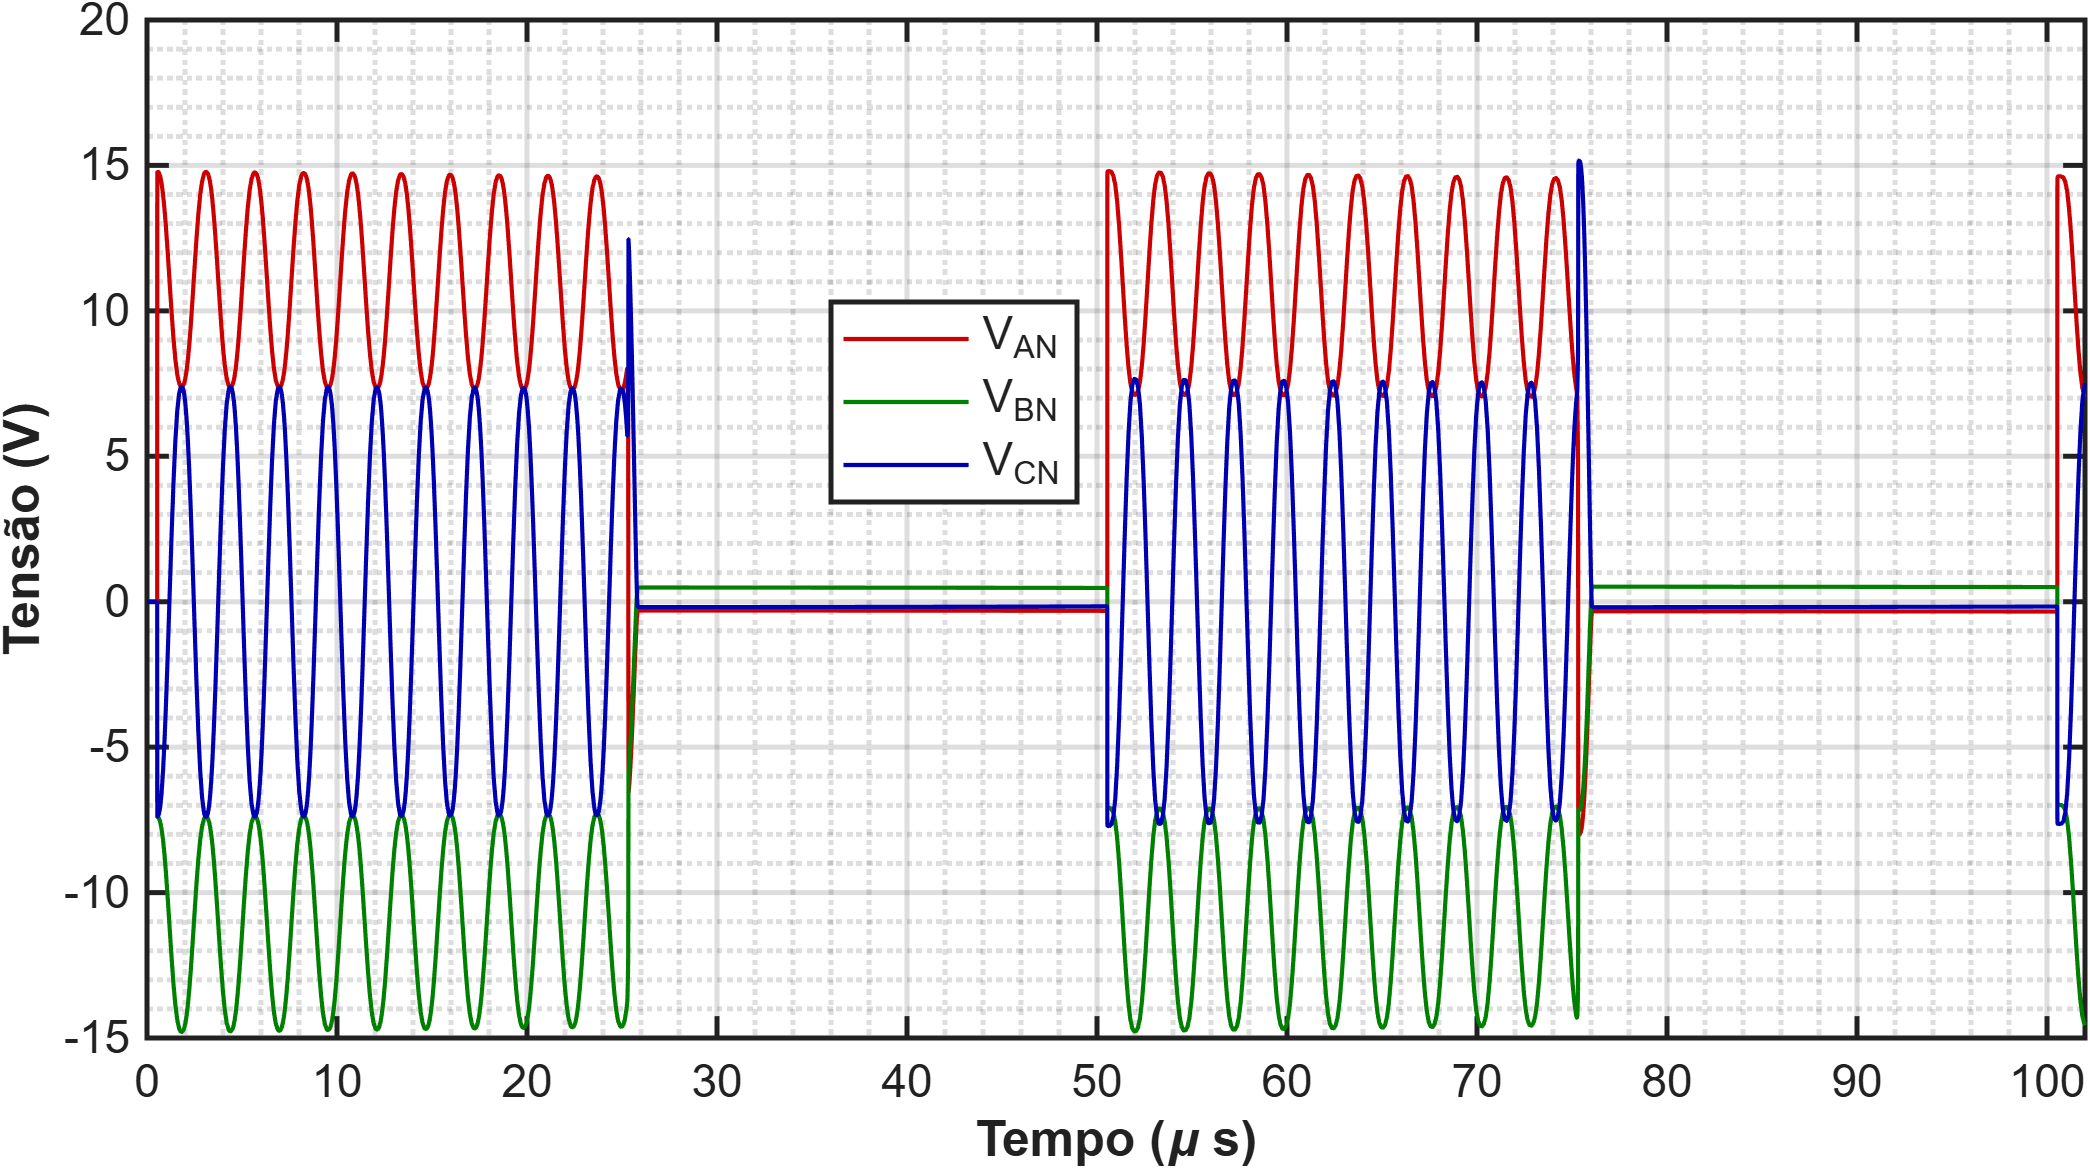
\includegraphics[width=0.8\textwidth]{Simulation/plot_simulacao/3_tensoes_fase_neutro.png}
    \caption*{Fonte: Elaborado pelo autor.}
    \label{fig:sim_tensoes_neutro}
\end{figure}


Do ponto de vista físico, o estabelecimento das tensões em $\pm 11,1 \: V$ é o resultado direto da divisão de potencial no fechamento em estrela (Y) do estator. Com a fase A submetida à tensão plena do barramento ($V_{DC} = 22,2 \: V$) e a fase B conectada ao referencial zero ($0 \: V$), o nó central (neutro) assume naturalmente o potencial médio exato de $11,1 \: V$. Ensaios paralelos nas Fases B e C confirmaram a manutenção do transístor inferior em condução plena ($15 \: V$) e os transistores da fase flutuante em corte ($0 \: V$), atestando a robustez da topologia contra disparos espúrios.

Comparando este resultado com os fundamentos da comutação trapezoidal detalhados na metodologia, a simulação valida a correta formação e estabilidade do potencial de neutro. Esta validação teórica prévia é de suma importância, pois ratifica a viabilidade da técnica de reconstrução de neutro virtual adotada no \textit{hardware}, assegurando que o microcontrolador possuirá uma referência de tensão simétrica e confiável para a detecção da Força Contraeletromotriz (FCEM) durante a operação em malha fechada.

A Figura \ref{fig:sim_bateria_esforco} demonstra o severo esforço transitório imposto à fonte de alimentação primária (bateria LiPo) quando conectada diretamente à ponte inversora, sem o auxílio de capacitores de barramento (\textit{Link DC}), o qual será inserido no projeto final. Observa-se como fato primário que, durante o \textbf{tempo de condução ($T_{on}$)}, a tensão da bateria decai gradualmente de $22,2 \: V$ para aproximadamente $21,9 \: V$, conforme ilustrado na Figura \ref{fig:bateria_tensao}. Esse comportamento acompanha a rampa de subida da corrente, que atinge o patamar de $13 \: A$. O fator mais crítico, no entanto, ocorre nos instantes exatos de comutação ($50 \: \mu s$ e $100 \: \mu s$), nos quais a corrente drena picos agudos que ultrapassam os $130 \: A$ e $200 \: A$, respectivamente, como detalhado na Figura \ref{fig:bateria_corrente}. Esses picos provocam quedas instantâneas (\textit{voltage sags}) severas na tensão da bateria, reduzindo-a para níveis próximos de $19,5 \: V$. Durante o \textbf{tempo de bloqueio ($T_{off}$)}, a corrente da bateria cessa completamente, pois a corrente do motor passa a circular em roda livre pelos diodos da ponte.

\begin{figure}[H]
    \centering
    \caption{Análise dinâmica dos parâmetros de entrada da bateria LiPo no Passo 1 sem filtragem capacitiva: (a) Transiente de tensão; (b) Transiente de corrente.}
    \label{fig:sim_bateria_esforco}
    \begin{subfigure}[b]{0.49\textwidth}
        \centering
        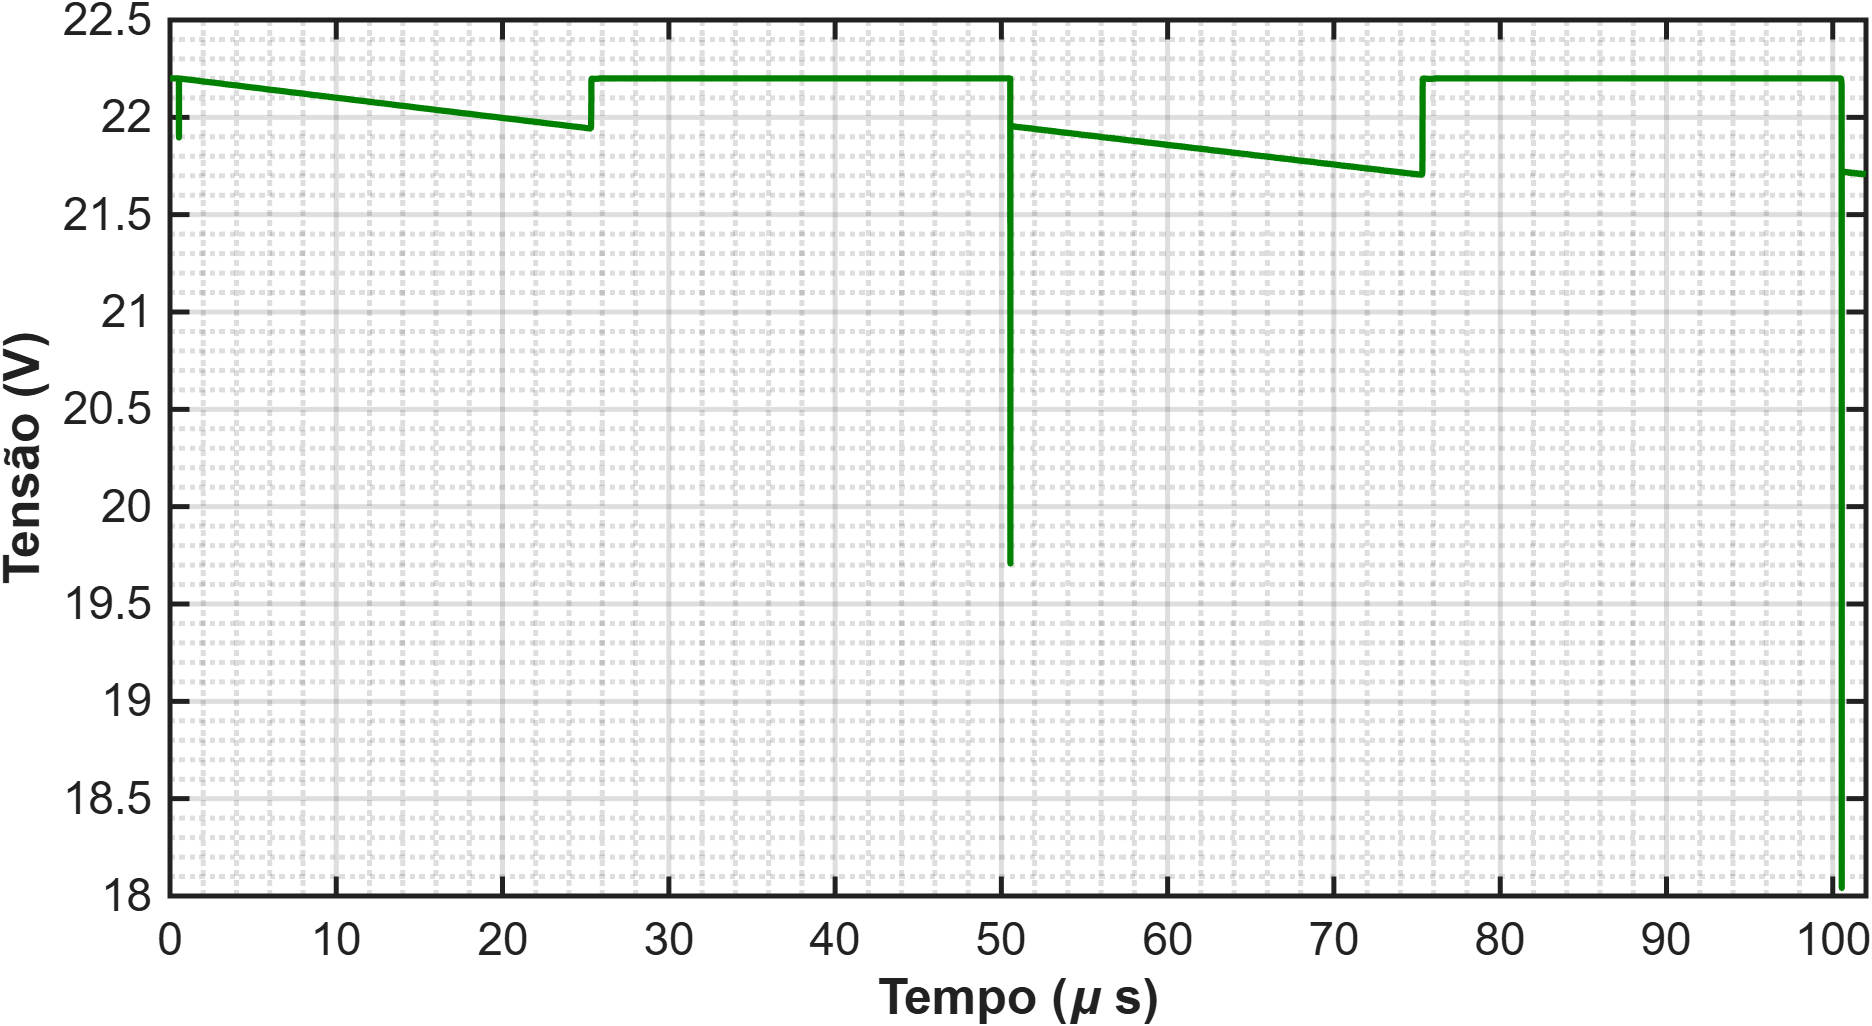
\includegraphics[width=\textwidth]{Simulation/plot_simulacao/7a_bateria_tensao.png}
        \caption{Tensão de barramento.}
        \label{fig:bateria_tensao}
    \end{subfigure}
    \hfill
    \begin{subfigure}[b]{0.49\textwidth}
        \centering
        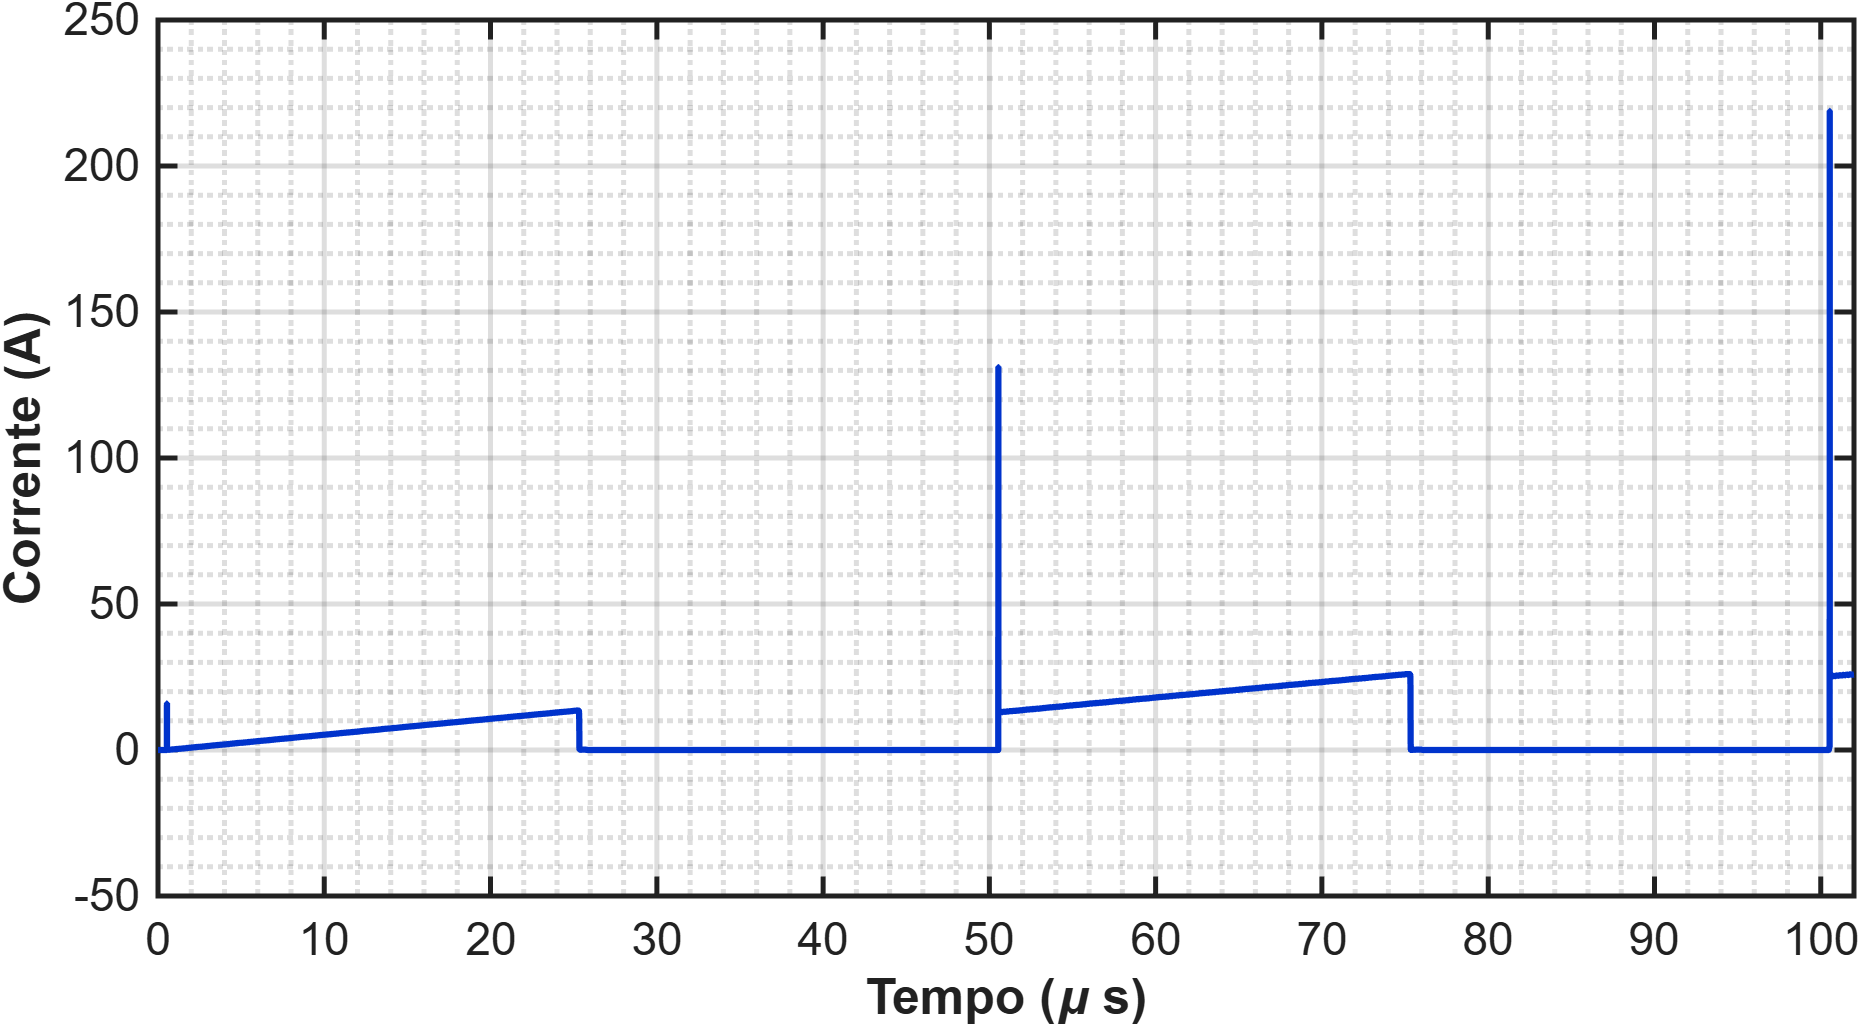
\includegraphics[width=\textwidth]{Simulation/plot_simulacao/7b_bateria_corrente.png}
        \caption{Corrente drenada.}
        \label{fig:bateria_corrente}
    \end{subfigure}
    \caption*{Fonte: Elaborado pelo autor.}
\end{figure}

A causa física para o decaimento gradual da tensão é a queda de potencial ôhmica intrínseca ($V_{drop} = I_a \cdot R_{ser}$) sobre a \textbf{resistência série equivalente} da bateria, que no modelo foi parametrizada como $19 \: m\Omega$. Por outro lado, os transientes agudos (\textit{spikes}) de corrente são consequência da elevadíssima taxa de variação ($di/dt$) exigida para carregar as capacitâncias parasitas dos MOSFETs e suprir a corrente de recuperação reversa (\textit{reverse recovery}) dos diodos corporais nos instantes de ativação (\textit{turn-on}). Como o circuito simulado neste ensaio possui apenas a bateria como fonte de energia, ela é forçada a fornecer instantaneamente toda a carga transitória.

A comparação deste comportamento simulado com a teoria de eletrônica de potência com o dimensionamento estabelecido na Metodologia. A simulação prova que submeter uma bateria LiPo a este nível de corrente de ondulação (\textit{ripple}) e picos transientes resultaria em superaquecimento severo e degradação química prematura das células. Fica, portanto, validada a necessidade imperativa da instalação do banco de \textbf{capacitores de filtro Low-ESR} ($940 \: \mu F$) projetado fisicamente na placa de circuito impresso (PCB), cuja função será atuar como um reservatório local de energia de baixíssima impedância para absorver estes transientes de alta frequência, isolando e protegendo a fonte primária.

\section{Projeto Eletrônico e Análise dos Esquemáticos}
%TODO: Inserir Introdução do capítulo.

\subsection{Circuito de Alimentação Auxiliar e Regulação}

A Figura \ref{fig:esquematico_supply} detalha a arquitetura de entrada e distribuição de energia do ESC. A conexão primária é realizada através de um conector de alta capacidade XT90, protegida imediatamente em série por um \textbf{fusível MIDI} de $80 \: A$ (modelo 0498080.M). O barramento DC (\textit{Link DC}) é suportado por um banco de capacitores híbrido em topologia paralela, composto por seis capacitores polarizados de $220 \: \mu F$ e três capacitores cerâmicos não polarizados de $1 \: \mu F$. A partir deste barramento filtrado, a tensão nominal da bateria alimenta dois módulos conversores \textit{buck} LM2596 dispostos em paralelo, responsáveis por gerar as malhas de tensão independentes de $15 \: V$ (\textit{Vcc 1}) e $5 \: V$ (\textit{Vcc 2}). Adicionalmente, o esquemático implementa uma separação explícita entre o \textbf{terra de potência (PGND)} e o \textbf{terra de sinal (SGND)}, interligados fisicamente por um único componente passivo limitador de laço (RJ1).

\begin{figure}[H]
    \centering
    \caption{Esquemático do estágio de entrada, filtragem do barramento DC e regulação de tensão auxiliar (Folha \textit{Supply}).}
    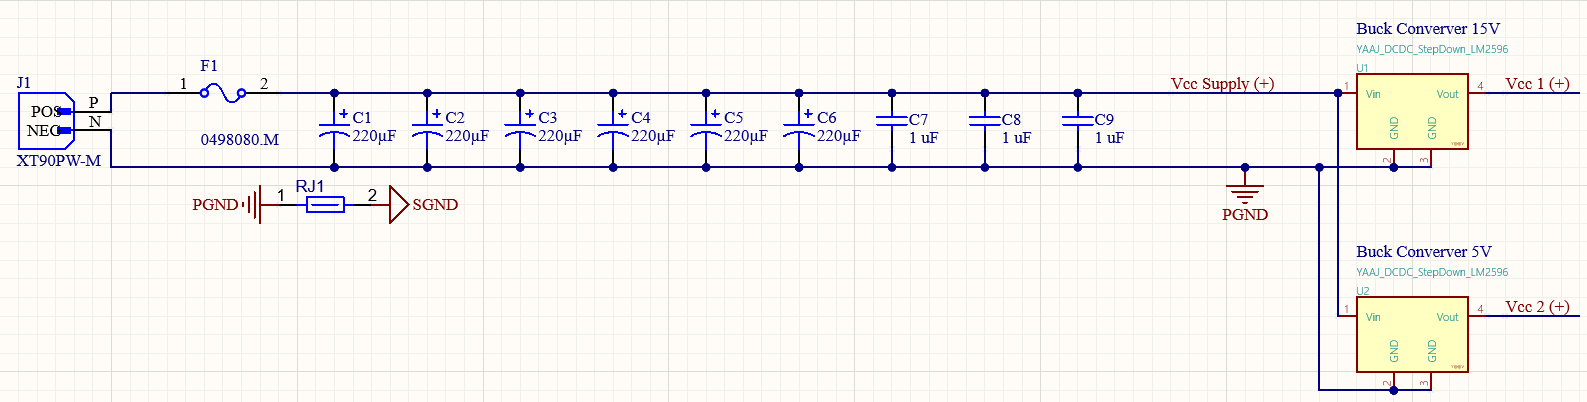
\includegraphics[width=1\textwidth]{imagens/esquematico_supply.png}
    \caption*{Fonte: Elaborado pelo autor.}
    \label{fig:esquematico_supply}
\end{figure}

Fisicamente, a divisão do banco capacitivo em múltiplas unidades de $220 \: \mu F$ reduz drasticamente a \textbf{Resistência Série Equivalente (ESR)} total do barramento, otimizando a absorção da elevada corrente de ondulação (\textit{ripple}) gerada pela ponte inversora sem causar aquecimento excessivo nos componentes. Os capacitores cerâmicos de $1 \: \mu F$ atuam no desacoplamento de alta frequência, suprimindo transientes que os capacitores eletrolíticos não conseguem filtrar devido à sua \textbf{Indutância Série Equivalente (ESL)}. A separação galvânica e o controle de retorno por meio da junção estrita entre \textbf{PGND} e \textbf{SGND} (\textit{Star Grounding}) impedem que as severas correntes de comutação do motor provoquem flutuações de tensão (\textit{ground bounce}) no referencial sensível do microcontrolador. 

A comparação com a metodologia teórica comprova a evolução e a robustez do projeto prático. Enquanto o texto preliminar previa genericamente a filtragem do \textit{Link DC} e reguladores em cascata, o arranjo físico adota conversores LM2596 dispostos em paralelo. Esta decisão elimina o gargalo térmico de fazer o regulador de menor tensão drenar corrente através do regulador primário, garantindo maior eficiência e isolamento entre o circuito de acionamento de \textit{gate} ($15 \: V$) e a lógica de processamento digital ($5 \: V$).

\subsection{Unidade de Processamento Lógico e Interface de Acionamento}

A Figura \ref{fig:esquematico_control} ilustra o núcleo de inteligência do ESC e sua interface direta com o estágio de potência. A Unidade de Processamento, baseada no módulo ESP32 (Figura \ref{fig:control_esp32}), é alimentada pela malha de $5 \: V$ (\textit{Vcc 2}). O regulador linear interno do microcontrolador reduz essa tensão para $3,3 \: V$, sinal que é exportado pelo pino 1 sob a nomenclatura \textit{Vmicro Ref}. Esta estratégia de projeto é fundamental: o \textit{Vmicro Ref} é roteado diretamente para os pinos de alimentação lógica (\textit{VDD}) dos três \textit{drivers} IR2110 (Figura \ref{fig:control_drivers}). Isso garante que o limiar de transição lógica (\textit{logic high threshold}) dos \textit{drivers} seja idêntico à tensão de saída dos pinos GPIO do ESP32, eliminando falhas de interpretação de sinal por incompatibilidade de níveis de tensão.

\begin{figure}[H]
    \centering
    \caption{Esquemáticos do núcleo de controle e interface de potência: (a) Microcontrolador ESP32-WROOM-32; (b) Estágio de translação de nível com \textit{drivers} IR2110.}
    \label{fig:esquematico_control}
    \begin{subfigure}[b]{0.48\textwidth}
        \centering
        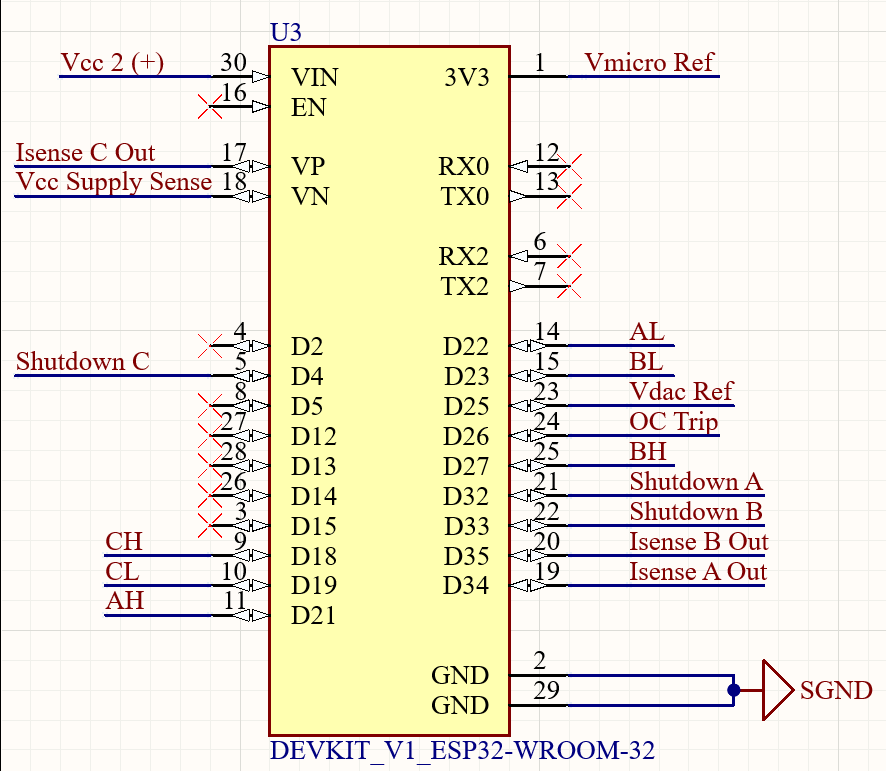
\includegraphics[width=\textwidth]{imagens/esp32_schematic.png}
        \caption{Unidade de Processamento (ESP32).}
        \label{fig:control_esp32}
    \end{subfigure}
    \hfill
    \begin{subfigure}[b]{0.48\textwidth}
        \centering
        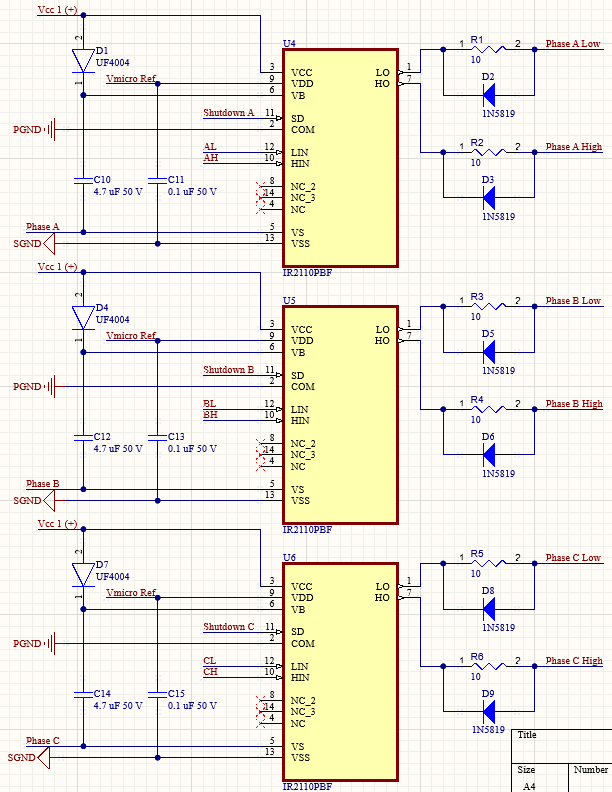
\includegraphics[width=\textwidth]{imagens/ir2110_schematic.png}
        \caption{\textit{Drivers} de \textit{Gate} (IR2110).}
        \label{fig:control_drivers}
    \end{subfigure}
    \caption*{Fonte: Elaborado pelo autor.}
\end{figure}

O isolamento contra ruídos é efetivado pela segregação dos planos de terra nos \textit{drivers} IR2110. O referencial lógico (\textit{VSS}) é conectado exclusivamente ao terra de sinal (\textbf{SGND}), enquanto o retorno de potência (\textit{COM}), que lida com os pulsos de alta corrente de carga e descarga dos MOSFETs, é roteado para o terra de potência (\textbf{PGND}). A comunicação de segurança entre o microcontrolador e os \textit{drivers} ocorre de forma redundante: o ESP32 gera os seis sinais do MCPWM ($AH, AL$, etc.) e possui controle direto sobre os pinos de \textit{Shutdown} ($SD$) de cada IR2110. Adicionalmente, o pino \textit{OC Trip} (\textit{Overcurrent Trip}) permite que um evento de falta detectado pelos sensores interrompa a geração de PWM no \textit{hardware} do ESP32 em microssegundos.

Na saída dos \textit{drivers}, o esquemático valida o projeto do circuito de \textit{bootstrap} e o condicionamento de \textit{gate}. A malha de \textit{bootstrap} utiliza um diodo de recuperação ultra-rápida (UF4004) alimentando uma associação capacitiva paralela ($4,7 \: \mu F$ e $0,1 \: \mu F$), combinando grande capacidade de reserva de carga com resposta instantânea a transientes. O acionamento dos MOSFETs foi projetado com uma topologia de \textbf{resistência de \textit{gate} assimétrica}: a ativação (\textit{turn-on}) é limitada pelos resistores de $10 \: \Omega$, amortecendo ressonâncias (\textit{ringing}) e picos de emissão eletromagnética (EMI). Em contrapartida, o bloqueio (\textit{turn-off}) ocorre através de diodos Schottky (1N5819) polarizados reversamente em paralelo com os resistores. Esta configuração fornece um caminho de baixíssima impedância para o escoamento imediato da carga do \textit{gate} ($Q_g$), garantindo que o transistor desligue mais rápido do que liga, prevenindo a ocorrência de condução cruzada (\textit{shoot-through}) no braço do inversor.

\pagebreak

\subsection{Condicionamento de Sinais e Sensoriamento}

A Figura \ref{fig:esquematico_sensors} detalha a topologia de aquisição de dados do inversor. Na Figura \ref{fig:sensor_voltage}, a tensão total do barramento (\textit{Vcc Supply}) é monitorada por um divisor resistivo de $39 \: k\Omega$ e $4,7 \: k\Omega$, resultando em um fator de atenuação de $0,1075$. Isso mapeia a tensão máxima da bateria 6S ($25,2 \: V$) para seguros $2,71 \: V$ no ADC do microcontrolador. Em contrapartida, na condição de alimentação com a tensão mínima projetada para o sistema (uma bateria 3S em seu limite de descarga operacional, com aproximadamente $9,0 \: V$), a tensão resultante no divisor será de $0,97 \: V$. Isso garante que toda a janela de operação mecânica e de alimentação do projeto permaneça estritamente dentro da faixa linear de leitura do ESP32, cujo limite lógico é $3,3 \: V$. Adicionalmente, o capacitor de $0,1 \: \mu F$, em conjunto com a resistência equivalente de Thévenin do divisor ($R_{th} \approx 4,19 \: k\Omega$), forma um filtro passa-baixa com frequência de corte ($f_c$) de aproximadamente $379 \: Hz$, como o sinal útil da queda de tensão da bateria é essencialmente contínuo ($0 \: Hz$), fixar a frequência de corte em $379 \: Hz$ empurra a frequência de chaveamento agressiva do inversor ($20 \: kHz$) quase duas décadas para dentro da banda de atenuação do filtro, caindo a uma taxa de $-20 \: dB/\text{década}$. Isso garante que as flutuações de comutação sejam suprimidas antes de atingirem o microcontrolador.

\begin{figure}[H]
    \centering
    \caption{Esquemáticos do estágio de sensoriamento e proteção: (a) Monitoramento da bateria; (b) Amplificadores de corrente das fases (INA240); (c) Comparadores de sobrecorrente (LM339).}
    \label{fig:esquematico_sensors}
    \begin{subfigure}[b]{0.32\textwidth}
        \centering
        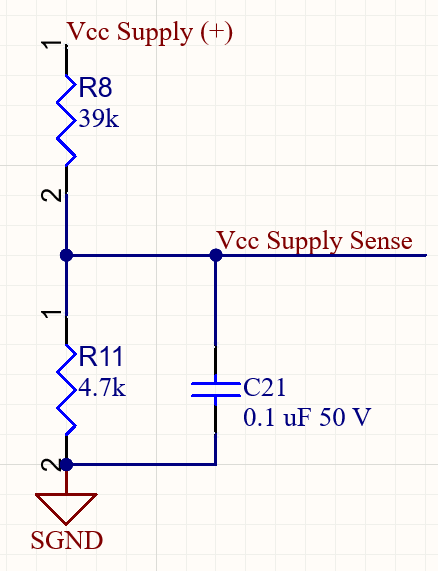
\includegraphics[width=\textwidth]{imagens/voltage_sense.png}
        \caption{Leitura de Tensão.}
        \label{fig:sensor_voltage}
    \end{subfigure}
    \hfill
    \begin{subfigure}[b]{0.32\textwidth}
        \centering
        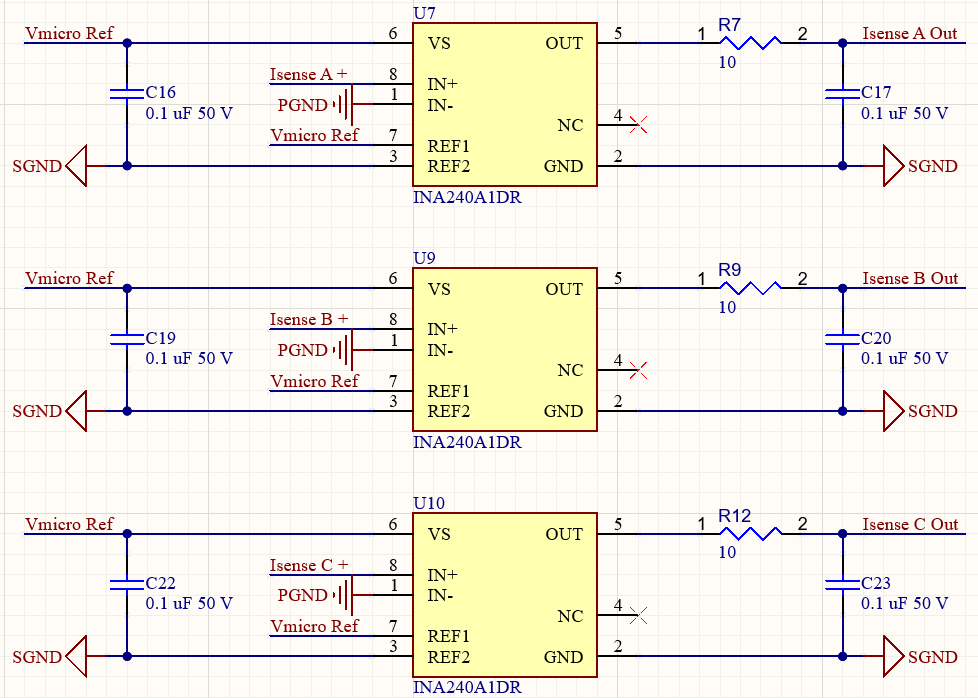
\includegraphics[width=\textwidth]{imagens/current_sense.png}
        \caption{Condicionamento de Corrente.}
        \label{fig:sensor_current}
    \end{subfigure}
    \hfill
    \begin{subfigure}[b]{0.32\textwidth}
        \centering
        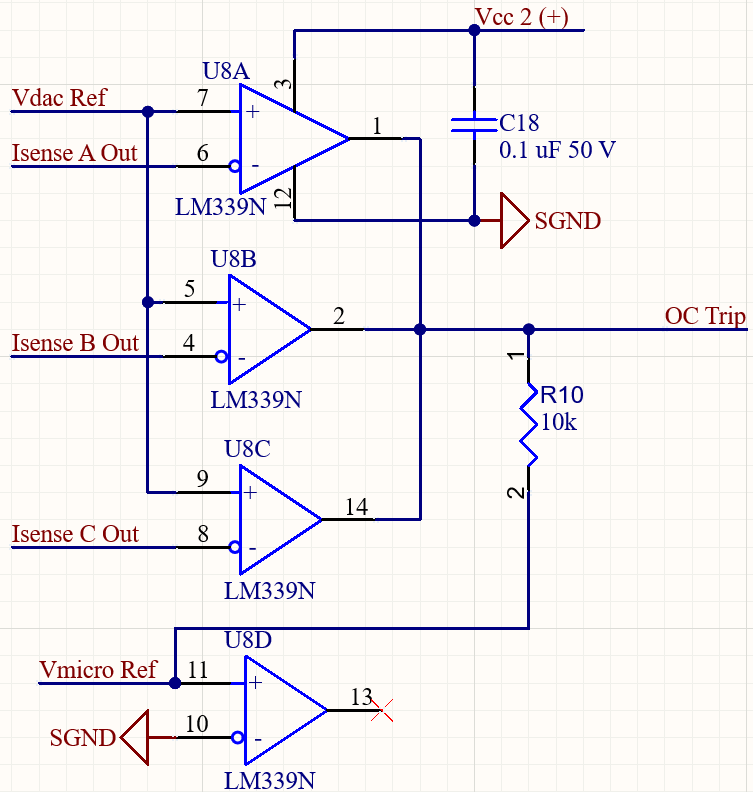
\includegraphics[width=\textwidth]{imagens/ocp_comparator.png}
        \caption{Proteção via \textit{Hardware} (OCP).}
        \label{fig:sensor_ocp}
    \end{subfigure}
    \caption*{Fonte: Elaborado pelo autor.}
\end{figure}

Foi adotado o circuito integrado \textbf{INA240A1DR} em cada fase (Figura \ref{fig:sensor_current}). Este componente é um amplificador de detecção de corrente, projetado especificamente com tecnologia de rejeição de PWM (\textit{Enhanced PWM Rejection}) para suprimir grandes variações de tensão ($dv/dt$) inerentes à comutação de motores. A versão A1DR possui um ganho fixo de $20 \: V/V$. Como as correntes nas bobinas de um motor BLDC são fisicamente alternadas (circulando nos dois sentidos), o microcontrolador seria incapaz de ler o semiciclo negativo, pois seu ADC suporta apenas tensões positivas ($0 \: V$ a $3,3 \: V$). Para viabilizar esta leitura, aplicou-se uma técnica de polarização diferencial: o pino \textit{REF1} foi ligado a $3,3 \: V$ (\textit{Vmicro Ref}) e o pino \textit{REF2} ao \textit{SGND} ($0 \: V$). O circuito do INA240 realiza a média aritmética dessas referências, estabelecendo um \textit{offset} interno exato de $1,65 \: V$ na saída. Consequentemente, uma corrente nula ($0 \: A$) repousa em $1,65 \: V$; correntes positivas elevam a saída em direção a $3,3 \: V$, enquanto correntes negativas a reduzem em direção a $0 \: V$. Este condicionamento garante a bidirecionalidade absoluta da medição, pré-requisito fundamental para a futura implementação de algoritmos avançados de Controle Orientado ao Campo (FOC).

A Figura \ref{fig:sensor_ocp} exibe o circuito de Proteção contra Sobrecorrente (OCP). O \textbf{LM339N} é um circuito integrado que encapsula quatro comparadores de tensão independentes, notável pela sua alta velocidade de reposta (na escala de nanossegundos) e pela sua arquitetura de saída em coletor aberto (\textit{open-collector}). Esta característica de coletor aberto é o que viabiliza a interligação das três proteções de fase em um único nó lógico (\textit{Wired-OR}), utilizando o resistor de \textit{pull-up} R10. Durante a revisão do projeto, realizou-se um ajuste topológico essencial nesta malha: a tensão limitadora (\textit{Vdac Ref}) foi conectada à porta não-inversora (+), enquanto o sinal dos sensores de corrente (\textit{Isense}) foi roteado para a porta inversora (-). Desta forma, em operação nominal ($Isense < Vdac$), os transistores de saída internos do LM339 permanecem em estado de corte (alta impedância), e o R10 mantém o pino \textit{OC Trip} em $3,3 \: V$. No instante em que qualquer fase individual superar o limite de segurança ($Isense > Vdac$), o seu respectivo comparador saturará, conduzindo a linha imediatamente ao terra ($0 \: V$). Esta ação puramente em \textit{hardware} contorna a latência intrínseca de qualquer \textit{software}, gerando uma interrupção prioritária no ESP32 para o bloqueio instantâneo do sinal PWM e salvaguardando a ponte inversora contra catástrofes térmicas ou elétricas.

\pagebreak

\subsection{Estágio de Potência e Ponte Inversora}

A Figura \ref{fig:esquematico_power} expõe a topologia final da ponte inversora trifásica, o núcleo de comutação de força do ESC. O arranjo utiliza seis transistores MOSFET IRFS7530-7PPBF de altíssima capacidade de corrente, estruturados em três braços independentes (Fases A, B e C). Para aumentar a confiabilidade dois detalhes de projeto merecem destaque: a inclusão de resistores de \textit{pull-down} de $10 \: k\Omega$ (R13 a R18) conectados aos terminais \textit{Gate-Source} de cada chave, e a alocação de três resistores \textit{shunt} de liga metálica (encapsulamento de potência 3920, modelo CSS2H-3920R-1L00F de $1 \: m\Omega$) inseridos especificamente nos ramos inferiores da ponte (\textit{Low-Side Sensing}).

\begin{figure}[H]
    \centering
    \caption{Esquemático do estágio de potência contendo a ponte inversora trifásica e resistores \textit{shunt} individuais para medição de corrente.}
    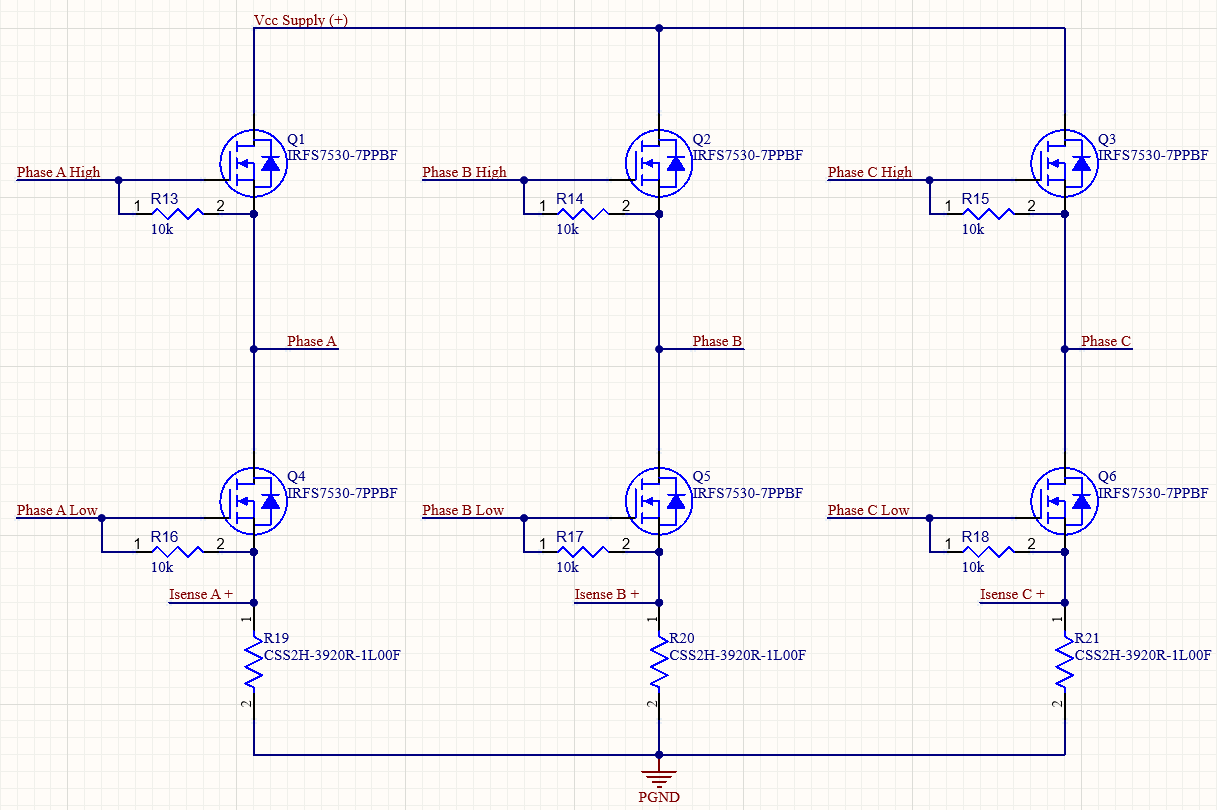
\includegraphics[width=0.9\textwidth]{imagens/esquematico_power.png}
    \caption*{Fonte: Elaborado pelo autor.}
    \label{fig:esquematico_power}
\end{figure}

A função física dos resistores de \textit{pull-down} é garantir um estado seguro de falha (\textit{fail-safe}). Durante a energização inicial do sistema (\textit{power-up}), reinicializações do microcontrolador ou em caso de rompimento físico das trilhas de acionamento, os \textit{gates} dos MOSFETs poderiam assumir um estado flutuante (alta impedância). Nesta condição, ruídos eletromagnéticos acoplados capacitivamente poderiam induzir o acionamento espúrio das chaves, resultando em um curto-circuito catastrófico direto no barramento DC (\textit{shoot-through}). Os resistores de $10 \: k\Omega$ asseguram que a tensão $V_{gs}$ permaneça rigidamente cravada em $0 \: V$ até que os \textit{drivers} IR2110 imponham ativamente o sinal de comando em $15 \: V$. 

Adicionalmente, em relação a escolha do invólucro de 7 pinos para os MOSFETs (D2PAK-7), este encapsulamento possui terminais múltiplos de \textit{Source}, o que minimiza a indutância parasita da pastilha de silício e atenua os anéis de oscilação (\textit{ringing}) durante os transientes de comutação de, no máximo, $90 \: A$. Já a topologia de sensoriamento de corrente no lado baixo (\textit{Low-Side}) atua como uma barreira de proteção para o estágio de condicionamento: em vez de expor os amplificadores INA240 às violentas oscilações de tensão de modo comum (\textit{Common-Mode Voltage}) que variam de $0 \: V$ a $25,2 \: V$ nos nós flutuantes das fases, a medição ocorre de forma referenciada ao terra da placa (\textit{PGND}). A queda de tensão medida sobre o \textit{shunt} de $1 \: m\Omega$ é da ordem de milivolts ($V = R \cdot I$), fornecendo um sinal extremamente limpo, seguro e proporcional à corrente exata que flui para o estator do motor.

\pagebreak

\subsection{Estratégias de Layout, Roteamento e Fabricação da PCB}

O projeto físico do inversor, ilustrado na Figura \ref{fig:pcb_layout}, foi materializado a partir de um laminado virgem de fibra de vidro (FR4) com dupla face de cobre nu, sem a aplicação de máscara de solda comercial (\textit{solder mask}). A placa possui dimensões de $150 \times 200 \: mm$ e espessura de $1,5 \: mm$. Durante a fase de engenharia de manufatura, o método de fabricação sofreu uma alteração: a confecção por corrosão química manual foi substituída pela usinagem em fresadora CNC (\textit{Computer Numerical Control}). A causa física para esta mudança baseia-se na precisão geométrica e na integridade do material condutor. Na corrosão de placas com imensas áreas de cobre, o processo tende a gerar \textit{undercutting} (corrosão lateral) e variações na espessura final da malha. A usinagem CNC atua de forma oposta, removendo mecanicamente apenas o material estritamente necessário para criar os isolamentos (\textit{clearances}), preservando a massa total e a espessura original do cobre contínuo. Para garantir a viabilidade da usinagem, as regras de \textit{design} (DRC) foram ajustadas para manter uma largura mínima de $0,6 \: mm$ nas trilhas de sinais lógicos e um \textit{clearance} mínimo de $0,6 \: mm$ entre elementos, prevenindo curtos-circuitos mecânicos e rompimentos de trilha durante a fresagem.

\begin{figure}[H]
    \centering
    \caption{Projeto de roteamento da Placa de Circuito Impresso no Altium Designer: (a) \textit{Top Layer} evidenciando os polígonos de potência; (b) \textit{Bottom Layer} evidenciando os planos de terra.}
    \label{fig:pcb_layout}
    \begin{subfigure}[b]{0.48\textwidth}
        \centering
        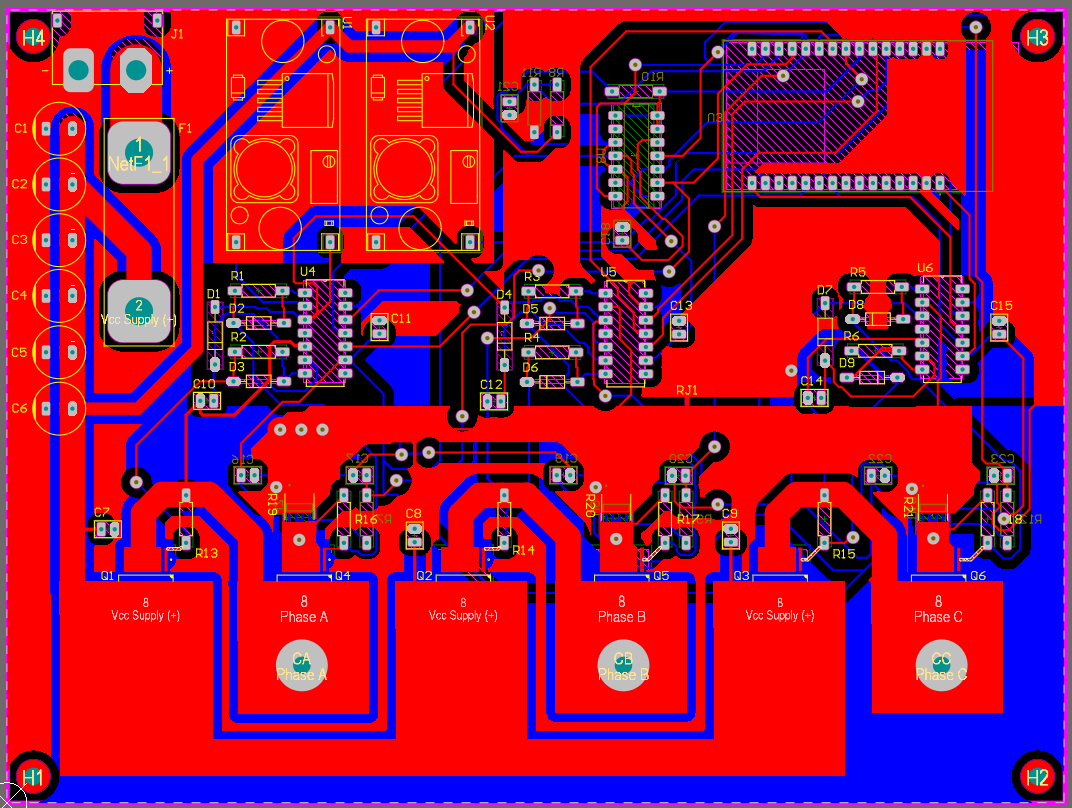
\includegraphics[width=\textwidth]{imagens/pcb_top.png}
        \caption{Camada Superior (\textit{Top Layer}).}
        \label{fig:pcb_top}
    \end{subfigure}
    \hfill
    \begin{subfigure}[b]{0.48\textwidth}
        \centering
        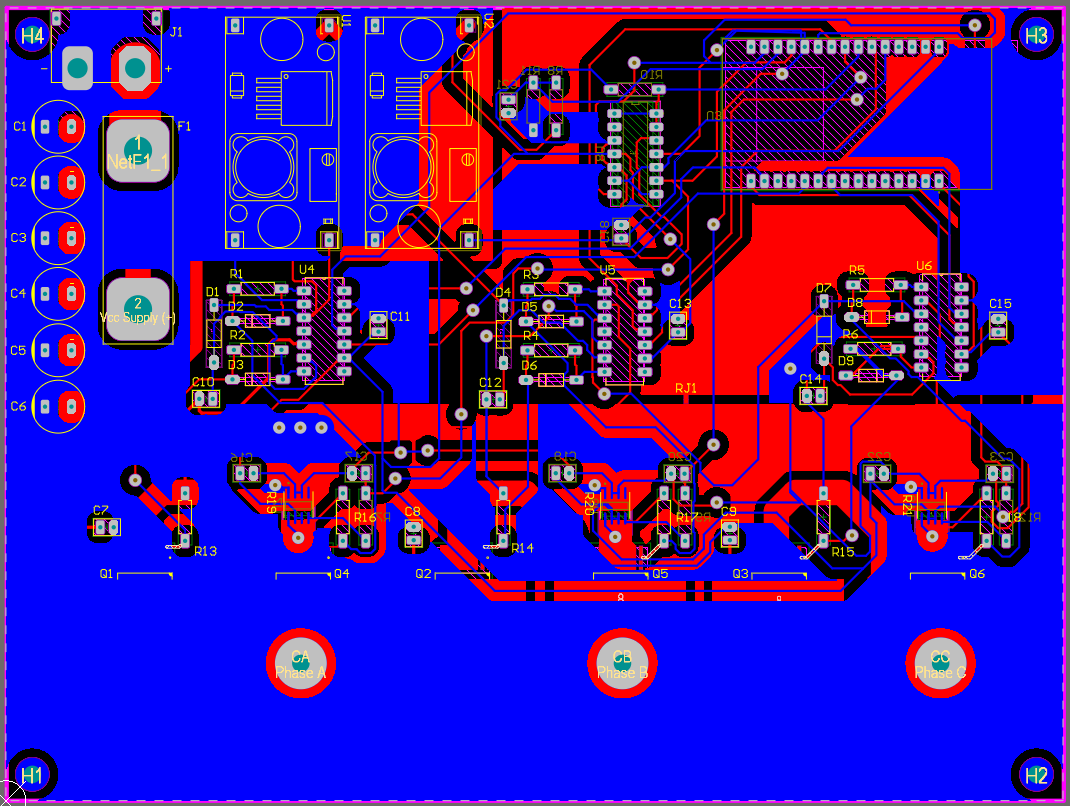
\includegraphics[width=\textwidth]{imagens/pcb_bottom.png}
        \caption{Camada Inferior (\textit{Bottom Layer}).}
        \label{fig:pcb_bottom}
    \end{subfigure}
    \caption*{Fonte: Elaborado pelo autor.}
\end{figure}

Embora as análises computacionais prévias tenham apontado transientes teóricos de comutação com picos próximos a $90 \: A$, ressalta-se que este protótipo inicial de bancada foi projetado para maximizar a capacidade de condução de corrente dentro das limitações físicas de fabricação local, não sendo esperado o regime de operação contínua sob esta magnitude extrema, já que de início o protótipo tem como objetivo demonstrar a viabilidade do design e será testado com um motor e bateria $4S$ e limitado a $3A$. 

Com o propósito de mitigar as perdas ôhmicas, o roteamento físico descartou o uso de trilhas convencionais em favor de grandes polígonos de preenchimento (\textit{copper pours}) sólidos. A camada superior (Figura \ref{fig:pcb_top}) acomoda as ilhas de comutação das fases e o barramento positivo, com gargalos projetados em um mínimo de $5 \: mm$ de largura. Contudo, como a espessura padrão do cobre de um laminado comum (tipicamente $1 \: oz/ft^2$ ou $35 \: \mu m$) possui uma secção transversal insuficiente para conduzir altas correntes, o sistema estaria sujeito à falha por superaquecimento térmico via Efeito Joule ($P = I^2 \cdot R_{trilha}$). Para contornar essa limitação e elevar o limite térmico do circuito, tirou-se proveito da própria natureza do material de prototipagem utilizado: o laminado de cobre nu. A ausência da máscara de solda isolante deixou todos os polígonos de potência naturalmente expostos. Esta característica facilitou a deposição manual de espessas camadas de liga de estanho e o assentamento de condutores de cobre sólido diretamente sobre as malhas críticas, aumentando substancialmente a área da secção transversal ($A$) das trilhas e reduzindo a sua resistência ôhmica equivalente ($\rho \cdot \frac{L}{A}$).

Do ponto de vista de compatibilidade eletromagnética (EMC), duas estratégias de isolamento foram rigorosamente aplicadas no layout. Primeiro, os espaços não roteados da placa foram preenchidos por dois imensos planos de terra funcionalmente segregados: o Terra de Potência (\textit{PGND}), concentrado na camada inferior (Figura \ref{fig:pcb_bottom}) sob o estágio do inversor, e o Terra de Sinal (\textit{SGND}), restrito à periferia dos circuitos lógicos e sensores. A conexão elétrica entre esses dois referenciais foi consolidada estritamente através da técnica de ponto único de aterramento (\textit{Star Ground}). Essa configuração impede o surgimento de laços de terra (\textit{ground loops}) e garante que as severas correntes de retorno induzidas pelo chaveamento do motor permaneçam confinadas na malha de potência, mitigando o fenômeno de flutuação de referencial (\textit{ground bounce}) sobre a eletrônica sensível. Segundo, a Unidade de Controle (ESP32) foi posicionada no extremo oposto da placa em relação aos MOSFETs. Como a comutação rápida de corrente gera campos magnéticos irradiados devido às altas taxas de $di/dt$, o distanciamento físico atua atenuando a intensidade do acoplamento indesejado de forma inversamente proporcional ao quadrado da distância, blindando o microcontrolador contra perturbações eletromagnéticas e travamentos espúrios.

\chapter{Conclusão}

O presente trabalho abordou o desenvolvimento de um protótipo de controlador eletrônico de velocidade (ESC) para motores de corrente contínua sem escovas (BLDC) utilizando o microcontrolador ESP32. O objetivo geral de estudar o princípio de funcionamento desses conversores e desenvolver uma plataforma física e lógica capaz de oferecer controle de velocidade e torque foi \textbf{parcialmente atingido}. Constatou-se que a arquitetura conceitual, o dimensionamento eletrônico preliminar e a implementação do \textit{firmware} alcançaram maturidade de engenharia consistente e foram validados em bancada. Contudo, a validação dinâmica integral com o motor em rotação não pôde ser concluída em razão de limitações físicas estruturais diagnosticadas no estágio de potência.

A metodologia adotada comprovou a viabilidade da topologia em malha aberta operando com comutação trapezoidal de seis passos. A arquitetura de \textit{firmware} modular demonstrou robustez, isolando as rotinas críticas de controle das tarefas secundárias. Os ensaios estáticos confirmaram a correta manipulação do periférico MCPWM, a eficácia do tempo morto (\textit{dead-time}) implementado por \textit{hardware} e o tempo de resposta adequado das proteções de sobrecorrente (OCP) e subtensão (UVLO).

O limite do escopo prático do protótipo foi estabelecido durante o ensaio a vazio, no qual a ponte inversora apresentou disparo da proteção da fonte primária devido ao consumo transiente excessivo de corrente sem carga acoplada. O diagnóstico metódico deste sintoma isolou a falha no estágio de potência físico, indicando a presença de um caminho de baixa impedância ou degradação de semicondutores em decorrência do estresse de chaveamento, exonerando a camada lógica de controle. Essa capacidade de rastreamento de falhas, evidenciada pela separação clara entre as limitações do \textit{hardware} prototipado e a estabilidade do \textit{software} desenvolvido, atesta a validade do processo investigativo adotado.

Para iterações futuras, a robustez do \textit{hardware} deve ser elevada mediante a adição de isolamento galvânico na interface lógica e a implementação de redes \textit{Snubber} com diodos TVS para a supressão de transientes no barramento. No que tange à integração, a arquitetura de acionamento requer a transição de \textit{drivers} discretos para \textit{Smart Gate Drivers} trifásicos, assegurando proteção nativa e absoluta contra intercondução (\textit{shoot-through}).

No aspecto da manufatura, a prova de conceito em tecnologia de furo passante (THT) cumpriu plenamente seu propósito de instrumentação e depuração inicial. O próximo estágio exige a migração para uma placa de circuito impresso (PCB) multicamadas estritamente SMD (\textit{Surface Mount Device}). Essa transição é essencial para minimizar as indutâncias parasitas, reduzir as sobretensões severas e atenuar a emissão de ruído eletromagnético inerente ao chaveamento em 20 kHz.

Com o \textit{hardware} de potência estabilizado, o \textit{firmware} já dispõe da infraestrutura base, incluindo o módulo de detecção de cruzamento por zero (ZCD) da força contraeletromotriz já codificado, para a validação da malha fechada \textit{sensorless}. Como passo subsequente, sugere-se a evolução do sistema para o Controle Vetorial Orientado a Campo (FOC) e a adoção do barramento CAN (\textit{Controller Area Network}) em substituição à telemetria Wi-Fi, adequando o ESC aos padrões de confiabilidade exigidos pela indústria automotiva e aeroespacial.

Em síntese, o trabalho entrega uma base arquitetural sólida, modular e extensamente documentada. As limitações práticas foram identificadas de forma analítica, consolidando um projeto que não se encerra em uma falha de bancada, mas estabelece um roteiro para a construção futura de controladores BLDC embarcados de alto desempenho.

% --- ELEMENTOS PÓS-TEXTUAIS ---
\postextual
\printbibliography

\end{document}
